% Options for packages loaded elsewhere
\PassOptionsToPackage{unicode}{hyperref}
\PassOptionsToPackage{hyphens}{url}
%
\documentclass[
  11pt,
  oneside]{book}
\usepackage{amsmath,amssymb}
\usepackage{iftex}
\ifPDFTeX
  \usepackage[T1]{fontenc}
  \usepackage[utf8]{inputenc}
  \usepackage{textcomp} % provide euro and other symbols
\else % if luatex or xetex
  \usepackage{unicode-math} % this also loads fontspec
  \defaultfontfeatures{Scale=MatchLowercase}
  \defaultfontfeatures[\rmfamily]{Ligatures=TeX,Scale=1}
\fi
\usepackage{lmodern}
\ifPDFTeX\else
  % xetex/luatex font selection
\fi
% Use upquote if available, for straight quotes in verbatim environments
\IfFileExists{upquote.sty}{\usepackage{upquote}}{}
\IfFileExists{microtype.sty}{% use microtype if available
  \usepackage[]{microtype}
  \UseMicrotypeSet[protrusion]{basicmath} % disable protrusion for tt fonts
}{}
\makeatletter
\@ifundefined{KOMAClassName}{% if non-KOMA class
  \IfFileExists{parskip.sty}{%
    \usepackage{parskip}
  }{% else
    \setlength{\parindent}{0pt}
    \setlength{\parskip}{6pt plus 2pt minus 1pt}}
}{% if KOMA class
  \KOMAoptions{parskip=half}}
\makeatother
\usepackage{xcolor}
\usepackage{longtable,booktabs,array}
\usepackage{calc} % for calculating minipage widths
% Correct order of tables after \paragraph or \subparagraph
\usepackage{etoolbox}
\makeatletter
\patchcmd\longtable{\par}{\if@noskipsec\mbox{}\fi\par}{}{}
\makeatother
% Allow footnotes in longtable head/foot
\IfFileExists{footnotehyper.sty}{\usepackage{footnotehyper}}{\usepackage{footnote}}
\makesavenoteenv{longtable}
\usepackage{graphicx}
\makeatletter
\def\maxwidth{\ifdim\Gin@nat@width>\linewidth\linewidth\else\Gin@nat@width\fi}
\def\maxheight{\ifdim\Gin@nat@height>\textheight\textheight\else\Gin@nat@height\fi}
\makeatother
% Scale images if necessary, so that they will not overflow the page
% margins by default, and it is still possible to overwrite the defaults
% using explicit options in \includegraphics[width, height, ...]{}
\setkeys{Gin}{width=\maxwidth,height=\maxheight,keepaspectratio}
% Set default figure placement to htbp
\makeatletter
\def\fps@figure{htbp}
\makeatother
\setlength{\emergencystretch}{3em} % prevent overfull lines
\providecommand{\tightlist}{%
  \setlength{\itemsep}{0pt}\setlength{\parskip}{0pt}}
\setcounter{secnumdepth}{5}
\usepackage{version}
\excludeversion{htmlonly}
\excludeversion{slidesonly}
\includeversion{notslides}
\usepackage{makeidx}
\makeindex
\usepackage{booktabs}
\usepackage{libertine}
%\usepackage{unicode-math}
%\setmathfont[Scale=MatchUppercase]{Libertinus Math}

\renewcommand{\chaptername}{}

\newcommand{\slide}{}
\newcommand{\cpybx}{}
\newcommand{\ecpybx}{}
\newbox{\copybox}

% \usepackage[x11names]{xcolor}
% \definecolor{Cream}{RGB}{254, 251, 237}
% \definecolor{Navy Blue}{RGB}{18,43,93}
% \pagecolor{Cream}
% \usepackage[paperwidth=4.6in,paperheight=3.25in,margin=4mm]{geometry}
% \setmainfont{TeX Gyre Heros}
% % \setmainfont{TeX Gyre Termes}
% \setmathfont{texgyretermes-math.otf}
% \renewcommand{\slide}{\vfill\eject}
% \renewcommand{\cpybx}{\setbox\copybox=\vbox\bgroup}
% \renewcommand{\ecpybx}{\egroup\copy\copybox}
% \color{Navy Blue}
% \pagestyle{empty}
% %% blanking solutions
% \usepackage{environ}
% \NewEnviron{blanksol}{\emph{Solution:}\vfill}
% \let\solution\blanksol
% \let\endsolution\endblanksol
\ifLuaTeX
  \usepackage{selnolig}  % disable illegal ligatures
\fi
\usepackage[]{natbib}
\bibliographystyle{plainnat}
\usepackage{bookmark}
\IfFileExists{xurl.sty}{\usepackage{xurl}}{} % add URL line breaks if available
\urlstyle{same}
\hypersetup{
  pdftitle={GENG0002 Mathematics B lecture notes},
  pdfauthor={Ján Špakula},
  hidelinks,
  pdfcreator={LaTeX via pandoc}}

\title{GENG0002 Mathematics B lecture notes}
\author{Ján Špakula}
\date{2024-03-07}

\usepackage{amsthm}
\newtheorem{theorem}{Theorem}[chapter]
\newtheorem{lemma}{Lemma}[chapter]
\newtheorem{corollary}{Corollary}[chapter]
\newtheorem{proposition}{Proposition}[chapter]
\newtheorem{conjecture}{Conjecture}[chapter]
\theoremstyle{definition}
\newtheorem{definition}{Definition}[chapter]
\theoremstyle{definition}
\newtheorem{example}{Example}[chapter]
\theoremstyle{definition}
\newtheorem{exercise}{Exercise}[chapter]
\theoremstyle{definition}
\newtheorem{hypothesis}{Hypothesis}[chapter]
\theoremstyle{remark}
\newtheorem*{remark}{Remark}
\newtheorem*{solution}{Solution}
\begin{document}
\maketitle

{
\setcounter{tocdepth}{1}
\tableofcontents
}
\chapter*{Front Matter}\label{front-matter}
\addcontentsline{toc}{chapter}{Front Matter}

These notes are based heavily on the notes provided over many years by a number of colleagues, notably A. Barney, V. Perisic, N. Petrosyan, and JH Renshaw.

I am still in the process of updating these and the online and PDF form of these notes may change in due course.

\chapter{Week 1}\label{week-one}

To start our exploration of the calculus, we start in lecture 1 with a look at the concept of limits of functions. We then consider the definition of the derivative of a function from first principles before looking at a few simple rules that enable us to evaluate some derivatives more easily than by first principles.
\slide

\section{Limits}\label{lecture-one}

In some cases, the value of a function at a point is undefined or cannot be determined. For example
\[
f(x) = \frac{x^2-9}{x-3}\tag{1}
\]
has the value \(\frac00\) for \(f(3)\), which is undetermined. However the function may still ``behave well'' around that point. In such cases it is convenient to introduce the idea of a limit or a limiting value.

Informally, a \textcolor{red}{\em limit}\index{limit} is a value which \(f(x)\) gets closer and closer to, but may never actually reach.

\slide

For example, the function \(f(x) = e^{-x}\) as it approaches the \(x-\)axis (Figure \ref{fig:01-exp-graph}).

\begin{figure}

{\centering 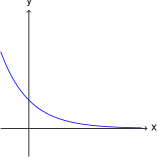
\includegraphics[width=0.41\linewidth]{fy-B-lectnotes_files/figure-latex/01-exp-graph-1} 

}

\caption{$e^{-x}$}\label{fig:01-exp-graph}
\end{figure}

\slide

In function (1) above, we can try to determine the limit \(f(x)\) as \(x\) gets closer to \(3\).
\[
f(x) = \frac{x^2-9}{x-3} = \frac{(x-3)(x+3)}{x-3} = x+3.
\]
(However, the last ``\(=\)'' is only valid for \(x\not=3\)!)

Now if \(x\) gets closer to \(3\), then \(x+3\) gets closer to \(6\). Formally we write
\[
\lim\limits_{x\to3} f(x) = 6
\]
and we say ``in the limit, if \(x\) tends to \(3\) then \(f(x)\) tends to 6''.

\slide

We can approach this in a slightly different way, by first letting \(x = a+3\) so that
\begin{align*}
f(x) &= f(a+3) = \frac{(a+3)^2-9}{(a+3)-3} = \frac{a^2+6a + 9 - 9}{a} =\\
&= \frac{a^2+6a}{a} = a+6.
\end{align*}
Now we can observe, that \(a\) gets closer to \(0\) if and only if \(x\) gets closer to \(3\). As \(a\) approaches \(0\) then \(f(a+3)\) approaches \(6\). So
\[
\lim\limits_{x\to3}f(x) = \lim\limits_{a\to0}f(a+3) = 6.
\]

(Why would we do this?)

\slide

Note that the limit is not the same thing as substituting the value of \(x=3\) into the function \(f(x)\), as \(f(x)\) is not defined at the value \(x=3\). We say that \(f\) is ``\emph{discontinuous}'' at \(x=3\).

A function \(f\) of \(x\) is said to be \textcolor{red}{\em continuous}\index{continuous} at the value \(x=a\) if:

\begin{itemize}
\tightlist
\item
  \(f\) is defined at \(a\), and
\item
  the value of the limit of \(f(x)\) as \(x\) tends to \(a\) is equal to \(f(a)\).
\end{itemize}

In other words
\[
\lim\limits_{x\to a}f(x) = f(a).
\]

Formally, a function \(f\) of \(x\) is said to be \textcolor{red}{\em discontinuous}\index{discontinuous} at \(x=a\) if it is not continuous at \(x=a\).
\slide

\begin{example}
Determine the limit of
\[
\frac{2x^2-5x-3}{x-3}
\]
as \(x\) tends to \(3\).
\end{example}

\begin{solution}
Let \(x = a+3\) so that as \(a\) tends to \(0\) then \(x\) tends to \(3\). Then
\[
f(a+3) = \frac{2(a+3)^2-5(a+3)-3}{(a+3)-3}=\frac{2a^2+12a+18-5a-15-3}{a}=\frac{2a^2+7a}{a} = a+7.
\]
So
\[
\lim\limits_{x\to3}\frac{2x^2-5x-3}{x-3} = \lim\limits_{x\to3}f(x) = \lim\limits_{a\to0}f(a+3) = \lim\limits_{a\to0}2a+7 = 7.
\]
Alternatively, you may spot that \(2x^2-5x-3 = (x-3)(2x+1)\) so that
\[
\lim\limits_{x\to 3}f(x) = \lim\limits_{x\to3}\frac{(x-3)(2x+1)}{x-3} = \lim\limits_{x\to3}2x+1 = 7.
\]
\end{solution}

\slide

\section{Differentiation from 1st Principles}\label{lecture-two}

For a straight line we can consider the \textcolor{red}{\em slope}\index{slope} or \textcolor{red}{\em gradient}\index{gradient}. This is a measure of how steep the line is, see Figure \ref{fig:02-gradient-line}.

\begin{figure}

{\centering 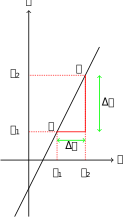
\includegraphics[width=0.3\linewidth]{fy-B-lectnotes_files/figure-latex/02-gradient-line-1} 

}

\caption{gradient of a line}\label{fig:02-gradient-line}
\end{figure}

\slide

The \textcolor{red}{\em gradient}\index{gradient} is defined to be the number
\[
\frac{\Delta y}{\Delta x} = \frac{y_2-y_1}{x_2-x_1}.
\]
For the line above, which has equation \(y = 2x-1\) then
\begin{align*}
\frac{\Delta y}{\Delta x} &= \frac{(2x_2-1)-(2x_1-1)}{x_2-x_1} = \frac{2(x_2-x_1)-1+1}{x_2-x_1}\\ &= \frac{2(x_2-x_1)}{x_2-x_1} = 2.
\end{align*}

\slide

Suppose now we are given a curve with equation \(y=f(x)\) and want to find the gradient of a line segment joining two points on the curve (Figure \ref{fig:03-line-seg-curve}).

\begin{figure}

{\centering 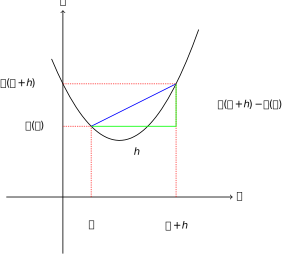
\includegraphics[width=0.7\linewidth]{fy-B-lectnotes_files/figure-latex/03-line-seg-curve-1} 

}

\caption{line segment of a curve}\label{fig:03-line-seg-curve}
\end{figure}

The gradient of this line segment is given by
\[
\frac{\Delta y}{\Delta x} = \frac{f(x+h)-f(x)}{h}.
\]
\slide

Notice that when \(h=0\) then this would have the indeterminate value of \(0/0\), and so the gradient is undefined when the two points on the line coincide. However, the limit of this expression, as \(h\to0\), may exist and it is instructive to imagine what the limit would represent geometrically (Figure \ref{fig:04-line-seg-curve2}):

\begin{htmlonly}

\phantomsection\label{div_head}
Let \(h\to 0\)

\phantomsection\label{div_body}

Press the button and see what happens to the line segment as \(h\to0\).

\end{htmlonly}

With some thought, it should be clear that the line segment tends to a line that just meets the curve at the point \((x,f(x))\), and we call this line the \textcolor{red}{\em tangent}\index{tangent} to the curve at the point \((x,f(x))\).

\begin{figure}

{\centering 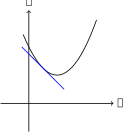
\includegraphics[width=0.7\linewidth]{fy-B-lectnotes_files/figure-latex/04-line-seg-curve2-1} 

}

\caption{line segment of a curve}\label{fig:04-line-seg-curve2}
\end{figure}

\slide

We call the slope of the tangent line the \textcolor{red}{\em derivative}\index{derivative} of the function \(y=f(x)\) at the point \(x\) and write
\[
\frac{\mathrm{d} f}{\mathrm{d} x} = \lim\limits_{h\to0}\frac{f(x+h)-f(x)}{h}
\]
and we refer to the process of calculating this limit as \textcolor{red}{\em differentiation by 1st principles}\index{differentiation by 1st principles}.

\slide

\begin{example}
Find the derivative by 1st principles for the function \(f(x) = x^2\) at the point \(x\).
\end{example}

\begin{solution}
\begin{gather*}
\frac{\mathrm{d} f}{\mathrm{d} x} = \lim\limits_{h\to0}\frac{f(x+h)-f(x)}{h} = \lim\limits_{h\to0}\frac{(x+h)^2 - x^2}{h} = \lim\limits_{h\to0}\frac{(x^2+2xh+h^2)-x^2}{h}\\ = \lim\limits_{h\to0}\frac{2xh+h^2}{h} = \lim\limits_{h\to0}(2x+h) = 2x.
\end{gather*}
\end{solution}

\slide

\begin{example}
Find the derivative by 1st principles for the function \(f(x) = x^3\) at the point \(x\).
\end{example}

\begin{solution}
\begin{gather*}
\frac{\mathrm{d} f}{\mathrm{d} x} = \lim\limits_{h\to0}\frac{f(x+h)-f(x)}{h} = \lim\limits_{h\to0}\frac{(x+h)^3 - x^3}{h} = \lim\limits_{h\to0}\frac{(x^3+3x^2h+3xh^2+h^3)-x^2}{h}\\ = \lim\limits_{h\to0}\frac{3x^2h+3xh^2+h^3}{h} = \lim\limits_{h\to0}(3x^2+3xh+h^2) = 3x^2.
\end{gather*}
\end{solution}

\slide

\begin{example}
Find the derivative by 1st principles for the function \(f(x) = 1/(2x-1)\) at the point \(x\).
\end{example}

\begin{solution}
Notice that
\begin{gather*}
f(x+h)-f(x) = \frac{1}{2(x+h)-1} - \frac{1}{2x-1} =\\ \frac{2x+1-\left(2(x+h)-1\right)}{\left(2(x+h)-1\right)\left(2x-1)\right)} = \frac{-2h}{(2x+2h-1)(2x-1)},
\end{gather*}
and so
\begin{gather*}
\frac{f(x+h)-f(x)}{h} = \frac{-2h}{h(2x+2h-1)(2x-1)} = \frac{-2}{(2x+2h-1)(2x-1)}.
\end{gather*}
Hence
\begin{gather*}
\frac{\mathrm{d} f}{\mathrm{d} x} = \lim\limits_{h\to0}\frac{f(x+h)-f(x)}{h} = \lim\limits_{h\to0}\frac{-2}{(2x+2h-1)(2x-1)} = \frac{-2}{(2x-1)(2x-1)} = \frac{-2}{(2x-1)^2}.
\end{gather*}
\end{solution}

\section{Differentiation by Rule}\label{lecture-three}

To summarise: we can differentiate a function by calculating a certain limit.

Can we do ``better'' so that we don't have to do this every time?

If we denote \(y = f(x)\), there are a few ways to \emph{denote} the derivative:
\[
\frac{\mathrm{d} f}{\mathrm{d} x} = \frac{\mathrm{d} y}{\mathrm{d} x} = f'(x).
\]
These all mean the same thing, namely the derivative of \(y=f(x)\) at the point \(x\), which is defined to be (recall)
\[
\frac{\mathrm{d} f}{\mathrm{d} x} = \lim\limits_{h\to0}\frac{f(x+h)-f(x)}{h}.
\]

\slide

\subsection{Rule for differentiation}\label{rule-for-differentiation}

Consider the differentiation of \(y = x^n\) from first principles. We have \(f(x+h) = (x + h)^n\).

Expanding the right-hand side using the binomial theorem gives
\[
f(x+h) = x^n + nx^{(n-1)}h+\frac{n(n-1)}{2!}x^{n-2}h^2+\ldots+h^n
\]
So that
\[
f(x+h)-f(x) = xn^{n-1}h+\frac{n(n-1)}{2!}x^{n-2}h^2+\ldots + h^n,
\]
and thus
\[
\frac{f(x+h)-f(x)}{h} = xn^{n-1}+\frac{n(n-1)}{2!}x^{n-2}h+\ldots + h^{n-1},
\]
\slide
Now, taking limit we have
\[
\frac{\mathrm{d} y}{\mathrm{d} x} = \lim\limits_{h\to0}\frac{f(x+h)-f(x)}{h} = nx^{n-1}.
\]
Therefore, in general, we can differentiate \(x^n\) for all values of \(n\) using the rule
\[
\frac{\mathrm{d} y}{\mathrm{d} x} = \frac{\mathrm{d} (x^n)}{\mathrm{d} x} = nx^{n-1}.
\]
This is known as the rule for differentiation (well, one of the rules, there is a number of them for various types of functions).
\slide

\begin{example}
Find the derivative by rule for the function \(y = x^4\) at the point \(x\).
\end{example}

\begin{solution}
\begin{gather*}
\frac{\mathrm{d} y}{\mathrm{d} x} = 4x^3.
\end{gather*}
\end{solution}

In words, the rule is: multiply the function by the exponent and then reduce the value of the exponent by one.

In fact this rule is also true for any real number in the exponent, not just when it is a positive integer.

\slide

\subsection{\texorpdfstring{Differentiation of \(ax^n\).}{Differentiation of ax\^{}n.}}\label{differentiation-of-axn.}

Where a power of \(x\) is multiplied by a constant, that constant remains unchanged by the process of differentiation. For example
\[
y = ax^n \Rightarrow \frac{\mathrm{d} y}{\mathrm{d} x} = nax^{n-1}.
\]

\begin{example}
Find the derivative by rule for the function \(y = 3x^4\) at the point \(x\).
\end{example}

\begin{solution}
\begin{gather*}
\frac{\mathrm{d} y}{\mathrm{d} x} = 3\times4x^3 = 12 x^3.
\end{gather*}
\end{solution}

\slide

Note that the derivative of \(ax\) and of \(a\) also follow the rule. For \(ax\) we may write \(ax = ax^1\). So differentiating by rule
\[
\frac{\mathrm{d} y}{\mathrm{d} x} = a\times1x^0 = a.
\]
For \(a\) we may write \(a = ax^0\) and hence differentiating by rule we have
\[
\frac{\mathrm{d} y}{\mathrm{d} x} = a\times0x^{-1} = 0.
\]
That is to say, the derivative of a constant value is always zero.

\slide

The above rule works in a more general situation. If \(f(x) = ag(x)\) where \(a\) is a constant and \(g(x)\) is a function, then
\begin{align*}
\frac{\mathrm{d} f}{\mathrm{d} x} &= \lim\limits_{h\to0}\frac{f(x+h)-f(x)}{h} = \lim\limits_{h\to0}\frac{ag(x+h)-ag(x)}{h} \\ &= a\lim\limits_{h\to0}\frac{g(x+h)-g(x)}{h} = a\frac{\mathrm{d} g}{\mathrm{d} x}.
\end{align*}

\slide

\subsection{Differentiation of a sum of terms}\label{differentiation-of-a-sum-of-terms}

If we have to differentiate more terms added together, then we differentiate each term separately and add them together. This is illustrated with the following example.

\begin{example}
Find the derivative by rule for the function \(y = 4x^5+3x^2-6x\) at the point \(x\).
\end{example}

\begin{solution}
\begin{gather*}
\frac{\mathrm{d} y}{\mathrm{d} x} = 4\times5x^4 + 3\times 2x^1 - 6\times1 = 20x^4+6x-6
\end{gather*}
\end{solution}

\slide

To summarise, so far we have the following rules for differentiation:

\begin{align*}
\frac{\mathrm{d}(x^n)}{\mathrm{d} x} &= nx^{n-1}\text{ for }n\in{\mathbb R}\\
\frac{\mathrm{d}(ag(x))}{\mathrm{d} x} &= a\frac{\mathrm{d} g}{\mathrm{d} x}\\
\frac{\mathrm{d}(f(x)+g(x))}{\mathrm{d} x} &= \frac{\mathrm{d} f}{\mathrm{d} x}+\frac{\mathrm{d} g}{\mathrm{d} x}.
\end{align*}
\slide

\section{Standard Derivatives}\label{standard-derivatives}

The derivatives in the following table are well-known and may be quoted without having to explain where they come from.

\begin{longtable}[]{@{}ll@{}}
\toprule\noalign{}
\(\mathbf{f(x)}\) & \(\mathbf{f'(x)}\) \\
\midrule\noalign{}
\endhead
\bottomrule\noalign{}
\endlastfoot
\(e^x\) & \(e^x\) \\
\(\ln(x)\) & \(\frac{1}{x}\) \\
\(\sin(x)\) & \(\cos(x)\) \\
\(\cos(x)\) & \(-\sin(x)\) \\
\(\tan(x)\) & \(\sec^2(x)\) \\
\(\csc(x)\) & \(-\csc(x)\cot(x)\) \\
\(\sec(x)\) & \(\sec(x)\tan(x)\) \\
\(\cot(x)\) & \(-\csc(x)\) \\
\end{longtable}

\chapter*{Week 1 Exercises}\label{week-1-exercises}
\addcontentsline{toc}{chapter}{Week 1 Exercises}

\section{Sheet 1 Limits}\label{sheet-1-limits}

\subsection*{Exercise 1}\label{exercise-1}
\addcontentsline{toc}{subsection}{Exercise 1}

Show that the following curves are continuous at the given \(x\) values by demonstrating that

\begin{enumerate}
\def\labelenumi{\alph{enumi}.}
\tightlist
\item
  \(\lim\limits_{x\to1}\frac{3x+2}{2x-1} = 5\);
\item
  \(\lim\limits_{x\to0}\frac{x+3}{x-2} = -\frac 32\);
\item
  \(\lim\limits_{x\to3}\frac{x^3+27}{x+3} = 9\);
\end{enumerate}

\slide

\subsection*{Exercise 2}\label{exercise-2}
\addcontentsline{toc}{subsection}{Exercise 2}

Determine the following limits:

\begin{enumerate}
\def\labelenumi{\alph{enumi}.}
\tightlist
\item
  \(\lim\limits_{x\to1}\frac{x^2+x-2}{x-1}\)
\item
  \(\lim\limits_{x\to2}\frac{2x^2-x-6}{x-2}\)
\item
  \(\lim\limits_{x\to2}\frac{x^2-4}{x-2}\)
\item
  \(\lim\limits_{x\to0}\frac{2x^2+3x}{x}\)
\item
  \(\lim\limits_{x\to2}\frac{x^2-x-2}{2x^2-3x-2}\)
\item
  \(\lim\limits_{x\to\infty}\frac{x}{2x+1}\)
\end{enumerate}

\slide

\subsection*{Exercise 3}\label{exercise-3}
\addcontentsline{toc}{subsection}{Exercise 3}

If \(f(x) = 3x^2\), determine \(\lim\limits_{h\to 0}\frac{f(x+h)-f(x)}{h}\).

\slide

\subsection*{Exercise 4}\label{exercise-4}
\addcontentsline{toc}{subsection}{Exercise 4}

If \(f(x) = x^2-2x\), determine \(\lim\limits_{h\to 0}\frac{f(x+h)-f(x)}{h}\).
\slide

{[}Solutions: 2. (a)3, (b) 7, (c) 4, (d) 3, (e) 3/5, (f) 1/2; 3. \(6x\); 4. \(2x-2\){]}
\slide

\section{Sheet 2 Differentiation by first principles}\label{sheet-2-differentiation-by-first-principles}

For each of the following functions differentiate \(y\) with respect to \(x\) from first principles.

\begin{enumerate}
\def\labelenumi{\arabic{enumi}.}
\tightlist
\item
  \(y=4x^2\)
\item
  \(y=6x^3\)
\item
  \(y=3x^2+2x\)
\item
  \(y=6x^2-4\)
\item
  \(y=3x^3+4x-5\)
\item
  \(y=x^4+x^2-3x\)
\item
  \(y=\frac{1}{x^2}\)
\item
  \(y=\frac{1}{5x+3}\)
\item
  \(y=\frac{1}{(1+x)^2}\)
\item
  \(y=x-\frac{2}{x}\)
\end{enumerate}

\slide

{[}Solutions: 1. \(y=8x\); 2. \(y=18x^2\); 3. \(y=6x+2\); 4. \(y=12x\); 5. \(y=9x^2+4\); 6. \(y=4x^3+2x-3\); 7. \(y=-2/x^3\); 8. \(y=-5/(5x+3)^2\); 9. \(y=-2/(1+x)^3\); 10. \(y=1+2/x^2\){]}

\slide

\section{Sheet 3 Differentiation by rule}\label{sheet-3-differentiation-by-rule}

Differentiate each of the following functions by rule:

\begin{tabular}{l|l}
\hline
 & \\
\hline
1. $y=x^7$ & 2. $y=6x^5$\\
\hline
3. $y=4x^3$ & 4. $s=0.5t^3$\\
\hline
5. $A=\pi r^2$ & 6. $y=x^{1/2}$\\
\hline
7. $s=0.2t^2$ & 8. $y=4x^{3/2}$\\
\hline
9. $y=2\sqrt{x}$ & 10. $y=3(\sqrt[3]{x^2})$\\
\hline
11. $y=\frac1{x^2}$ & 12. $y=\frac 1x$\\
\hline
13. $y=\frac3{5x}$ & 14. $y=\frac2{x^3}$\\
\hline
15. $y=\frac1{\sqrt{x}}$ & 16. $y=\frac2{3\sqrt{x}}$\\
\hline
17. $y=\frac5{x\sqrt{x}}$ & 18. $s=3\frac{\sqrt{t}}5$\\
\hline
19. $k=\frac{0.01}{h}$ & 20. $y=\frac5x$\\
\hline
21. $y=4x^2-3x+2$ & 22. $s=3t^3-2t^2+5t-3$\\
\hline
23. $q=2u^2-u+7$ & 24. $y=5x^4-7x^3+3x^2-2x$\\
\hline
25. $s=7t^5-3t^2+7$ & 26. $y=3.1x^{1.5}-2.4x^{0.6}$\\
\hline
27. $y=\frac{x+x^3}{\sqrt{x}}$ & 28. $y=\frac{3+x^2}x$\\
\hline
29. $y=\sqrt{x}+\frac1{\sqrt{x}}$ & 30. $y=x^3+\frac3{\sqrt{x}}$\\
\hline
31. $t^{1.3}-\frac1{4t^{2.3}}$ & 32. $y=\frac{3x^3}5-\frac{2x^2}7-\sqrt{x}$\\
\hline
33. $y=0.008+\frac{0.001}{x}$ & 34. $s=10-6t+7t^2-2t^3$\\
\hline
\end{tabular}
\slide

{[}Solutions: 1. \(dy/dx=7x^6\); 2. \(dy/dx=30x^4\); 3. \(dy/dx=12x^2\); 4. \(ds/dt=1.5t^2\); 5. \(dA/dr=2\pi r\); 6. \(dy/dx=1/(2x^{1/2})\); 7. \(ds/dt=0.4t\); 8. \(dy/dx=6x^{1/2}\); 9. \(dy/dx=1/\sqrt{x}\); 10. \(dy/dx=2/\sqrt[3]{x}\); 11. \(dy/dx=-2/x^3\); 12. \(dy/dx=-1/x^2\); 13. \(dy/dx=-3/(5x^2)\); 14. \(dy/dx=-6/x^4\); 15. \(dy/dx=-1/(2x^{3/2})\); 16. \(dy/dx=-1/(3x^{3/2})\); 17. \(dy/dx=-15/(2x^{5/2})\); 18. \(ds/dt=3/(10\sqrt{t})\); 19. \(dk/dh=-0.01/h^2\); 20. \(dy/dx=-5/x^2\); 21. \(dy/dx=8x-3\); 22. \(ds/dt=9t^2-4t+5\); 23. \(dq/du=4u-1\); 24. \(dy/dx=20x^3-21x^2+6x-2\); 25. \(ds/dt=35t^4-6t\); 26. \(dy/dx=4.65x^{0.5}-1.44/x^{0.4}\); 27. \(dy/dx=1/(2x^{1/2})+5x^{3/2}/2\); 28. \(dy/dx=-3/x^2+1\); 29. \(dy/dx=1/(2\sqrt{x})-1/(2x\sqrt{x})\); 30. \(dy/dx=3x^2-3/(2x^{3/2})\); 31. \(ds/dt=1.3t^{0.3}+0.575/t^{3.3}\); 32. \(dy/dx=9x^2/5-4x/7-1/(2\sqrt{x})\); 33. \(dy/dx=-0.001/x^2\); 34. \(ds/dt=-6+14t-6t^2\){]}

\chapter{Week 2}\label{week-two}

This week we will consider the equations of tangents and normals and then complete our rules for differentiation by looking at

\begin{enumerate}
\def\labelenumi{\arabic{enumi}.}
\tightlist
\item
  Chain rule
\item
  Product rule
\item
  Quotient rule.
\end{enumerate}

\slide

\section{Tangents and Normals}\label{lecture-four}

Two lines are \textcolor{red}{\em parallel}\index{parallel} if their gradients are identical. For example \(y=2x\), \(y=2x-2\) and \(y=2x+3\) all have gradient of \(2\) and hence are all parallel (Figure \ref{fig:05-parallel-lines}).

\begin{figure}

{\centering 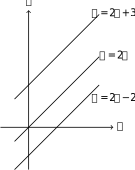
\includegraphics[width=0.4\linewidth]{fy-B-lectnotes_files/figure-latex/05-parallel-lines-1} 

}

\caption{parallel lines}\label{fig:05-parallel-lines}
\end{figure}
\slide

If two lines are perpendicular, there is also a certain relationship between their gradients. Consider Figure \ref{fig:06-perpendicular-lines}.

\begin{figure}

{\centering 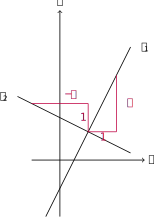
\includegraphics[width=0.4\linewidth]{fy-B-lectnotes_files/figure-latex/06-perpendicular-lines-1} 

}

\caption{perpendicular lines}\label{fig:06-perpendicular-lines}
\end{figure}
\slide

The gradient of the line \(l_1\) is given by the ratio
\[
\frac{m}{1},
\]
while the gradient of the line \(l_2\) is given by the ratio
\[
\frac{1}{-m}.
\]
So if a line has gradient \(m\) then the gradient of the line perpendicular to it has gradient \(-1/m\), and so
\[
\text{gradient of }(l_1) \times \text{ gradient of }(l_2) = -1.
\]
\slide
Now consider Figure \ref{fig:07-tangent-and-normal}.

\begin{figure}

{\centering 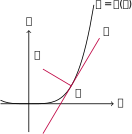
\includegraphics[width=0.4\linewidth]{fy-B-lectnotes_files/figure-latex/07-tangent-and-normal-1} 

}

\caption{tangent and normal}\label{fig:07-tangent-and-normal}
\end{figure}
\slide

The \textcolor{red}{\em normal}\index{normal} is the line at \(90^\circ\) to the tangent, passing through the point where the tangent touches the curve. Thus in the figure, the tangent is the line \(PT\) and the normal is the line \(PN\). We already know that the gradient of the tangent is given by
\[
m = \frac{\mathrm{d} y}{\mathrm{d} x}\text{ at the point }P,
\]
and so from the argument above, the gradient of the normal to the tangent is given by
\[
\frac{-1}{m} = \frac{-1}{{\mathrm{d} y/\mathrm{d} x}}.
\]
Now, the equation of the line with gradient \(m\), passing through the point \(P=(x_1,y_1)\) is given by
\[
y-y_1 = m(x-x_1).
\]
So the \textcolor{red}{\em equation of the tangent}\index{equation of the tangent} is
\[
y - y_1 = \frac{\mathrm{d} y}{\mathrm{d} x}(x-x_1),
\]
while the \textcolor{red}{\em equation of the normal}\index{equation of the normal} to the curve is
\[
y - y_1 = \frac{-1}{{\mathrm{d} y/\mathrm{d} x}}(x-x_1).
\]
\slide

\begin{example}
Find the equation of the tangent and the normal to the curve \(y = x^2+5x\) at the point \(x=2\).
\end{example}

\begin{solution}
If \(y=x^2+5\) then \({\mathrm{d} y/\mathrm{d} x} = 2x+5\).

At \(x_1=2\), \(y_1 = 2^2 + 5\times2 = 14\) and \({\mathrm{d} y/\mathrm{d} x} = 2\times2+5=9\).
The equation of the tangent is therefore
\[
y-14=9(x-2) = 9x - 18\text{ and so }y = 9x-4.
\]
The equation of the normal is
\[
y-14=\frac{-1}{9}(x-2) = \frac{-1}{9}x - \frac{2}{9}\text{ and so }y = -\frac{x}{9}+\frac{128}{4}.
\]
\end{solution}

\slide

\section{The Chain Rule}\label{lecture-five}

A function may be considered as an operation that has to be done to \(x\) to get \(y\). For example if \(y = f(x) = x^2\) then the function (called \(f\) in this case) is: square the value of \(x\).

For \(y = g(\theta) = \sin(\theta)\) the function (called \(g\) in this case) is: evaluate the sine of \(\theta\).

If we now look at \((x^2 + 4)^3\) then we can consider this as one function described be performing these steps:

\begin{enumerate}
\def\labelenumi{\arabic{enumi}.}
\tightlist
\item
  take \(x\),
\item
  square it,
\item
  add \(4\) to the previous result, and then
\item
  cube the preceding result.
\end{enumerate}

\slide

So we can write
\[
y = f(x) = (x^2+ 4)^3,
\]
or we can think of \(f\) as (a composition of) two functions:
\begin{align*}
u &= g(x) = x^2 + 4\\
y &= h(u) = u^3,
\end{align*}
or we can even consider it as (a composition of) 3 functions:
\begin{align*}
u &= k(x) = x^2\\
v &= m(u) = u + 4\\
y &= n(v) = v^3.
\end{align*}
\slide
In the first case, the value of \(y\) is calculated all in one attempt. In the second case, \(u\) is calculated from \(x\) according to the rule of the function \(g\), then \(y\) is calculated using \(u\) and the rule of the function \(h\). In the third case \(u\) is calculated from \(x\) according to the rule \(k\), then \(v\) is calculated from \(u\) according to the rule \(m\), and finally \(y\) is calculated from the value of \(v\) according to the rule \(n\).

We shall consider the second case. Recall:
\begin{align*}
u &= g(x) = x^2+ 4\\
y &= h(u) = u^3.
\end{align*}
By substituting for \(u\) we can write \(y = h(g(x))\) which means: to get \(y\) from \(x\), first apply the rule \(g\) (get \(x\), square it and add \(4\)) and then apply the rule \(h\) (cube the answer to operation \(g\)). When \(y\) is written in this form it is called a \textcolor{red}{\em function of a function}\index{function of a function} or a \textcolor{red}{\em composite functon}\index{composite functon}.
\slide

\subsection{The Chain Rule: Differentiating composite functions}\label{the-chain-rule-differentiating-composite-functions}

Let consider the function \(y = (x^2+ 4)^3\). Up to now, if we wanted to differentiate \(y = (x^2 + 4)^3\), we had to multiply out the brackets to get a string of things added together, since so far the only things we can differentiate are sums of terms of standard functions (e.g.~\(\sin(x), \cos(x), \ln(x)\), etc).

The chain rule allows us to differentiate functions of functions without having to multiply out all the brackets.

\slide

Recall that we ``decompose'' \(y=(x^2+4)^3\) as \(u = g(x) = x^2+4\), \(y = h(u) = u^3\).
Thus
\[
\frac{\mathrm{d} y}{\mathrm{d} u} = 3u^2 \quad\text{ and }\quad
\frac{\mathrm{d} u}{\mathrm{d} x} = 2x
\]
(using ordinary differentiation by rule).

However, we want to find
\[
\frac{\mathrm{d} y}{\mathrm{d} x}.
\]
The \textcolor{red}{\em chain rule}\index{chain rule} says that
\[
\frac{\mathrm{d} y}{\mathrm{d} x} = \frac{\mathrm{d} y}{\mathrm{d} u}\times \frac{\mathrm{d} u}{\mathrm{d} x}.
\]
(This can be proved from first principles, but we won't.)
So
\[
\frac{\mathrm{d} y}{\mathrm{d} x} = \frac{\mathrm{d} y}{\mathrm{d} u}\times \frac{\mathrm{d} u}{\mathrm{d} x} = 3u^2\times 2x = 6xu^2.
\]
But since \(u = x^2+4\), we have
\[
\frac{\mathrm{d} y}{\mathrm{d} x} = 6x(x^2 +4)^2.
\]

\begin{remark}
The chain rule can be extended for any number of functions, for example
\[
\frac{\mathrm{d} y}{\mathrm{d} x} = \frac{\mathrm{d} y}{\mathrm{d} a}\times \frac{\mathrm{d} a}{\mathrm{d} b}\times \frac{\mathrm{d} b}{\mathrm{d} c}\times \frac{\mathrm{d} c}{\mathrm{d} e}\times\frac{\mathrm{d} e}{\mathrm{d} f}\times\frac{\mathrm{d} f}{\mathrm{d} x}.
\]
\end{remark}

\slide

\begin{example}
Differentiate \(s = (2t^2- 4t)^5\) with respect to \(t\).
\end{example}

\begin{solution}
Let \(u = 2t^2-4t\) and \(s = u^5\). Then
\[
\frac{\mathrm{d} u}{\mathrm{d} t} = 4t-4\text{ and }\frac{\mathrm{d} s}{\mathrm{d} u} = 5u^4
\]
So
\[
\frac{\mathrm{d} s}{\mathrm{d} t} = \frac{\mathrm{d} s}{\mathrm{d} u}\times\frac{\mathrm{d} u}{\mathrm{d} t} = 5u^4(4t-4).
\]
But since \(u = 2t^2-4t\) then
\[
\frac{\mathrm{d} s}{\mathrm{d} t} = 5(2t^2-4t)^4(4t-4).
\]
\end{solution}

\slide

\begin{example}
Differentiate \(y=5\cos(5\theta)\) with respect to \(\theta\).
\end{example}

\begin{solution}
Let \(u = 5\theta\) and \(y = 5\cos(u)\). Then
\[
\frac{\mathrm{d} u}{{\mathrm{d} \theta}} = 5\text{ and }\frac{\mathrm{d} y}{\mathrm{d} u} = -5\sin(u)
\]
So
\[
\frac{\mathrm{d} y}{{\mathrm{d} \theta}} = \frac{\mathrm{d} y}{\mathrm{d} u}\times\frac{\mathrm{d} u}{{\mathrm{d} \theta}} = -5\sin(u)\times5.
\]
But since \(u = 5\theta\) then
\[
\frac{\mathrm{d} y}{{\mathrm{d} \theta}} = -25\sin(5\theta).
\]
\end{solution}

\slide

\begin{example}
Differentiate \(y=e^{2x+3}\) with respect to \(x\).
\end{example}

\begin{solution}
Let \(u = 2x+3\) and \(y = e^u\). Then
\[
\frac{\mathrm{d} u}{\mathrm{d} x} = 2\text{ and }\frac{\mathrm{d} y}{\mathrm{d} u} = e^u
\]
So
\[
\frac{\mathrm{d} y}{\mathrm{d} x} = \frac{\mathrm{d} y}{\mathrm{d} u}\times\frac{\mathrm{d} u}{\mathrm{d} x} = e^u\times2.
\]
But since \(u = e^u\) then
\[
\frac{\mathrm{d} y}{\mathrm{d} x} = 2e^{2x+3}.
\]
\end{solution}

\slide

\section{The Product and Quotient Rules}\label{lecture-six}

\subsection{Differentiation of a product}\label{differentiation-of-a-product}

So far, if we want to differentiate a function which is a product of two functions of \(x\), like \(y = 4x^2(3x^3 - 6x)\), we need to multiply out the brackets and differentiate term by term as follows;
\begin{gather*}
y = 4x^2(3x^3 - 6x) = 12x^5 - 24x^3\\
\frac{\mathrm{d} y}{\mathrm{d} x} = 60x^4 - 72x^2 = 12x^2(5x^2 - 6)
\end{gather*}
For some products, multiplying terms out still doesn't help to differentiate them e.g.
\[
y = \sqrt{x^2 - 2x} \sin(x).
\]
(We could use binomial expansion for the first factor, but we still don't have tools to turn \(\sin(x)\) into a power series.)
\slide

We'd like a general rule for differentiating a product.

From the first example above, we see that the derivative of a product is not just the derivative of each factor, as
that would give \(8x(9x^2 - 6) = 72x^3 - 48x\).

Let \(u = u(x)\) and \(v = v(x)\) be functions of \(x\).

If \(y = u(x)v(x)\), then \(y(x+h) = u(x+h)v(x+h)\), so
\[y(x+h)-y(x) = u(x+h)v(x+h) - u(x)v(x).\]
Now we do a trick: add and subtract \(u(x+h)v(x)\):
\begin{align*}
y(x+h)-y(x) &= u(x+h)v(x+h) - u(x+h)v(x)\\
    &\phantom{=} + u(x+h)v(x) - u(x)v(x).
\end{align*}
\slide
Further, dividing both sides of equation by \(h\) gives
\begin{align*}
\frac{y(x+h)-y(x)}{h} &= u(x+h)\frac{v(x+h) - v(x)}{h} \\
 &\phantom{=} + v(x)\frac{u(x+h ) - u(x)}{h}.
\end{align*}
In the limit as \(h\) tends to \(0\), we have \(u(x+h)\to u(x)\), and so
\[ 
\frac{\mathrm{d} y}{\mathrm{d} x} = u\frac{\mathrm{d} v}{\mathrm{d} x} + v\frac{\mathrm{d} u}{\mathrm{d} x}.
\]
Equivalently,
\[ 
\frac{\mathrm{d}(uv)}{\mathrm{d} x} = u\frac{\mathrm{d} v}{\mathrm{d} x} + v\frac{\mathrm{d} u}{\mathrm{d} x}.
\]
This is called the \textcolor{red}{\em product rule}\index{product rule}.
\slide

\begin{example}
Differentiate \(y=4x^2(3x^3-6x)\) with respect to \(x\).
\end{example}

\begin{solution}
Let \(u = 4x^2\) and \(v = 3x^3-6x\). Then
\[
\frac{\mathrm{d} u}{\mathrm{d} x} = 8x\text{ and }\frac{\mathrm{d} v}{\mathrm{d} x} = 9x^2-6.
\]
Hence the product rule gives
\begin{gather*}
\frac{\mathrm{d} y}{\mathrm{d} x} = u\frac{\mathrm{d} v}{\mathrm{d} x} + v\frac{\mathrm{d} u}{\mathrm{d} x} = (3x^3-6x)\times 8x + 4x^2\times(9x^2-6)\\
24x^4 - 48x^2 + 36x^4-24x^2 = 60x^4-72x^2 = 12x^2(5x^2-6).
\end{gather*}
\end{solution}

\slide

\begin{example}
Differentiate \(y=\sqrt{x^2-2x}\sin(x)\) with respect to \(x\).
\end{example}

\begin{solution}
Let \(u = \sqrt{x^2-2x} = (x^2-2x)^{1/2}\) and \(v = \sin(x)\). Then
\[
\frac{\mathrm{d} u}{\mathrm{d} x} = \frac12(x^2-2x)^{-1/2}(2x-2)=(x^2-2x)^{-1/2}(x-1)\text{ and }\frac{\mathrm{d} v}{\mathrm{d} x} = \cos(x).
\]
Hence the product rule gives
\begin{gather*}
\frac{\mathrm{d} y}{\mathrm{d} x} = u\frac{\mathrm{d} v}{\mathrm{d} x} + v\frac{\mathrm{d} u}{\mathrm{d} x} = (x^2-2x)^{1/2}\cos(x) + \sin(x)(x^2-2x)^{-1/2}(x-1)\\
\frac{(x-1)\sin(x)}{(x^2-2x)^{1/2}} + (x^2-2x)^{1/2}\cos(x).
\end{gather*}
\end{solution}

\slide

\subsection{Differentiation of a quotient}\label{differentiation-of-a-quotient}

Suppose that
\[
y = \frac{u(x)}{v(x)} = \frac{u}{v}.
\]
Considering a small \(h\), we have \(y(x+h) = \dfrac{u(x+h)}{v(x+h)}\).
Hence
\begin{align*}
y(x+h)-y(x) &= \frac{u(x+h)}{v(x+h)} - \frac{u(x)}{v(x)}\\
&=\frac{v(x)u(x+h)-u(x)v(x+h)}{v(x+h)v(x)}\\
&=\tfrac{v(x)u(x+h)-v(x)u(x)+v(x)u(x)-u(x)v(x+h)}{v(x+h)v(x)}.
\end{align*}
\slide
Dividing by \(h\) and rearranging, we get
\[
\frac{y(x+h)-y(x)}{h} = \frac{v(x)\frac{u(x+h)-u(x)}{h}+u(x)\frac{v(x)-v(x+h)}{h}}{v(x+h)v(x)}.
\]
Thus in the limit as \(h\) tends to zero
\[\frac{\mathrm{d} y}{\mathrm{d} x} = \lim\limits_{h\to0}\frac{y(x+h)-y(x)}{h} = \frac{v(x)\frac{\mathrm{d} u}{\mathrm{d} x} - u(x)\frac{\mathrm{d} v}{\mathrm{d} x}}{v(x)^2}
\]

This is the formula for the \textcolor{red}{\em differentiation of a quotient}\index{differentiation of a quotient}.

Note that for the product formula it is up to you which part of the product you call \(u\) and which \(v\), but that for the quotient formula, the denominator of the quotient must be \(v\) and the numerator must be \(u\).
\slide

There is an alternative way to derive this formula. Since
\[
y = \frac{u(x)}{v(x)} = u(x)v(x)^{-1}
\]
and since \(v(x)^{-1}\) is a composite of the function \(v(x)\) and the function \(x^{-1}\), we can use a combination of the product rule and the chain rule. So
\begin{align*}
\frac{\mathrm{d}(uv^{-1})}{\mathrm{d} x} &= u\frac{\mathrm{d}(v^{-1})}{\mathrm{d} x}+v^{-1}\frac{\mathrm{d} u}{\mathrm{d} x} = u\left(-1\times v^{-2}\frac{\mathrm{d} v}{\mathrm{d} x}\right) + v^{-1}\frac{\mathrm{d} u}{\mathrm{d} x}\\
&= \frac{\mathrm{d} u}{\mathrm{d} x}\frac{1}{v} - \frac{u}{v^2}\frac{\mathrm{d} v}{\mathrm{d} x} = \frac{v\frac{\mathrm{d} u}{\mathrm{d} x}-u\frac{\mathrm{d} v}{\mathrm{d} x}}{v^2}.
\end{align*}
\slide

\begin{example}
Differentiate \(y=\frac{3x^2+2}{(4x^2-4)^2}\) with respect to \(x\).
\end{example}

\begin{solution}
Let \(u = 3x^2+2\) and \(v = (4x^2-4)^2\).
Then
\[
\frac{\mathrm{d} u}{\mathrm{d} x} = 6x\text{ and }\frac{\mathrm{d} v}{\mathrm{d} x} = 2(4x^2-4)\times8x = 16x(4x^2-4)
\]
and so
\[
\frac{\mathrm{d} y}{\mathrm{d} x} = \frac{v\frac{\mathrm{d} u}{\mathrm{d} x}-u\frac{\mathrm{d} v}{\mathrm{d} x}}{v^2} = \frac{(4x^2-4)^26x - (3x^2+2)16x(4x^2-4)}{((4x^2-4)^2)^2} = \frac{6x(4x-4)-16x(3x^2+2)}{(4x^2-4)^3}.
\]
\end{solution}

\slide

\begin{example}
Differentiate \(y=\frac{1-\sin(x)}{1+\sin(x)}\) with respect to \(x\).
\end{example}

\begin{solution}
Let \(u = 1-\sin(x)\) and \(v = 1+\sin(x)\).
Then
\[
\frac{\mathrm{d} u}{\mathrm{d} x} = -\cos(x)\text{ and }\frac{\mathrm{d} v}{\mathrm{d} x} = \cos(x) 
\]
and so
\[
\frac{\mathrm{d} y}{\mathrm{d} x} = \frac{v\frac{\mathrm{d} u}{\mathrm{d} x}-u\frac{\mathrm{d} v}{\mathrm{d} x}}{v^2} = \frac{(1+\sin(x)(-\cos(x))-(1-\sin(x))(\cos(x))}{(1+\sin(x))^2} = \frac{-2\cos(x)}{(1+\sin(x))^2}.
\]
\end{solution}

\chapter*{Week 2 Exercises}\label{week-2-exercises}
\addcontentsline{toc}{chapter}{Week 2 Exercises}

\section{Sheet 4 Tangents and Normals}\label{sheet-4-tangents-and-normals}

\subsection*{Exercise 1}\label{exercise-1-1}
\addcontentsline{toc}{subsection}{Exercise 1}

In each of the examples below determine the equations of the tangent and normal at the point indicated.

\begin{enumerate}
\def\labelenumi{\alph{enumi}.}
\tightlist
\item
  \(y=x^2\) at the point where \(x=1\),
\item
  \(y=2x^2-3x\) at the point where \(x=2\),
\item
  \(y=1+x-x^2\) at the point where \(x=2\),
\item
  \(y=x^3-5x+3\) at the point where \(x=3\),
\item
  \(y=1/x\) at the point where \(x=2\),
\item
  \(y=(x-3)^2\) at the point where \(x=5\).
\end{enumerate}

\slide

\subsection*{Exercise 2}\label{exercise-2-1}
\addcontentsline{toc}{subsection}{Exercise 2}

Determine the gradient for \(y=6x^3-9x^2-20x+6\) and show that the slope is zero when \(x=5/3\) and when \(x=-2/3\). Establish the gradient at \(x=1\) and then write the equations of the tangent and the normal to the curve at this point.

\slide

{[}Solutions. 1: (a) \(y=2x-1\)/\(y=-x/2+3/2\); (b) \(y=5x-8\)/\(y=-x/5+12/5\); (c) \(y=-3x+5\)/\(y=x/3-5/3\); (d) \(y=22x-51\)/\(y=-x/22+333/22\); (e) \(y=-x/4+1\)/\(y=4x-15/2\); (f) \(y=4x-16\)/\(y=-x/4+21/4\)

2: \(dy/dx = 18x^2-18x-20 = 0\) gives \(x=5/3\) and \(x=-2/3\). \(dy/dx(1) = -20\). Equation of tangent is \(y=-20x+3\), equation of normal is \(y=x/20-341/20\).{]}

\slide

\section{Sheet 5 The Chain Rule}\label{sheet-5-the-chain-rule}

Differentiate each of the following functions using the chain rule.

\begin{enumerate}
\def\labelenumi{\arabic{enumi}.}
\tightlist
\item
  \(y=(2x+5)^2\)
\item
  \(y=(1-5x)^4\)
\item
  \(s=(3t+t)^5\)
\item
  \(p=(1-2q^2)^{11}\)
\item
  \(y=(1-2x)^3\)
\item
  \(y=(3x^2-5x+4)^4\)
\item
  \(s=(4t^3+3t-2)^2\)
\item
  \(y=\frac1{\sqrt{x^2-1}}\)
\item
  \(y=a\sin(a\theta)\)
\item
  \(y=\sin(\omega t)\)
\item
  \(y=\cos(2\pi ft+\frac{\pi}2)\)
\item
  \(y=\tan(4x+3)\)
\item
  \(y=6e^{5x}\)
\item
  \(y=\ln(2x^5)\)
\item
  \(y=\ln(\frac 1x)\)
\end{enumerate}

\slide

\{Solutions. (1) \(dy/dx=8x+20\); (2) \(dy/dx=-20(1-5x)^3\); (3) \(ds/dt=15(3t+7)^4\); (4) \(dp/dq=-44q(1-2q^2)^{10}\); (5) \(dy/dx=-6(1-2x)^2\); (6) \(dy/dx=(24x-20(3x^2-5x+4)^3\); (7) \(ds/dt=(24t^2+6)(4t^3+3t-2)\); (8) \(dy/dx=-x/(x^2-1)^{3/2}\); (9) \(dy/d\theta=a^2\cos(a\theta)\); (10) \(dy/d\omega=\omega\cos(\omega t)\); (11) \(dy/dt=-2\pi f\sin(2\pi ft+\pi/2)\); (12) \(dy/dx=4\sec^2(4x+3)\); (13) \(dy/dx=30e^{5x}\); (14) \(dy/dx=5/x\); (15) \(dy/dx=-1/x\)\}
\slide

\section{Sheet 6 The Product Rule}\label{sheet-6-the-product-rule}

\[
\text{if }y(x)=u(x)v(x)\text{ then }dy/dx=udv/dx+vdu/dx
\]
Differentiate the following functions

\begin{enumerate}
\def\labelenumi{\arabic{enumi}.}
\tightlist
\item
  \(y=(4x+5)(x^2-2x)\)
\item
  \(y=x^{5/3}(4x-2)^2\)
\item
  \(y=(x+1)^2(1-2x)\)
\item
  \(y=4x\sqrt{5-2x^2}\)
\item
  \(y=(4x^2+3x)(2x-8)^5\)
\item
  \(y=8x^3\sin(3x)\)
\item
  \(y=4x^2\cos(x)\)
\item
  \(y=(x^2-2x)\sin(x)\)
\item
  \(y=e^{2x}\sin(x)\)
\item
  \(y=x\ln(x)\)
\item
  \(y=\sqrt{x^2+4}\cos(2x+1)\)
\item
  \(y=\sqrt{x^2-1}\ln(2x+1)\)
\item
  \(y=e^{x\ln(x)}\)
\item
  \(y=x^x\)
\end{enumerate}

\slide

\{Solutions. 1. \((4x+5)(2x-2)+4(x^2-2x)\); 2. \(8x^{5/3}(4x-2)+5x^{2/3}(4x-2)^2/3\); 3. \(-2(x+1)^2+2(1-2x)(x+1)\); 4. \(-8x^2(5-2x^2)^{-1/2}+4(5-2x^2)^{1/2}\); 5. \(10(4x^2+3x)(2x-8)^4+(8x+3)(2x-8)^5\); 6. \(24x^2\sin(3x)+24x^3\cos(3x)\); 7. \(8x\cos x-4x^2\sin(x)\); 8. \((2x-2)\sin(x)+(x^2-2x)\cos(x)\); 9. \(2e^{2x}\sin(x)+e^{2x}\cos(x)\); 10. \(\ln(x)+1\); 11. \(x(x^2+4)^{-1/2}\cos(2x+1)-2(x^2+4)^{1/2}\sin(2x+1)\); 12. \(x(x^2-1)^{-1/2}\ln(2x+1)+2\sqrt{x^2-1}/(2x+1)\); 13. \(\exp(x\ln x)(1+\ln x)\); 14. same as 13.\}
\slide

\section{Sheet 7 The Quotient Rule}\label{sheet-7-the-quotient-rule}

Differentiate the following functions with respect to \(x\) using the quotient rule

\begin{enumerate}
\def\labelenumi{\arabic{enumi}.}
\tightlist
\item
  \(y=\frac{3x^2+2}{5x+4}\)
\item
  \(y=\frac{(9x^2+3)^2}{2x-8}\)
\item
  \(y=\frac{1+x}{1-x}\)
\item
  \(y=\frac{2x+2}{(3x^3+2x)^2}\)
\item
  \(y=9x^2-\frac{x^2+2x}{1-x}\)
\item
  \(y=\frac{3x-4}{2x^2+1}\)
\item
  \(y=\frac{\sin(3x)}{x+1}\)
\item
  \(y=\frac{4x(3x-4)^2}{\sin(x)}\)
\end{enumerate}

\slide

\{Solutions: 1. \(dy/dx = (15x^2+24x-10)/(5x+4)^2\); 2. \(dy/dx = 18(3x^2+1)(9x^2-48-1)/(2x-8)^2\); 3. \(dy/dx = 2/(1-x)^2\); 4. \(dy/dx = -2(3x^3+2x)(15x^3+18x^2+2x+4)/(3x^3+2x)^4\); 5. \(dy/dx = 18x+(x^2-2x-2)/(1-x)^2\); 6. \(dy/dx = (-6x^2+16x+3)/(2x^2+1)^2\); 7. \(dy/dx = (3\cos(3x)(x+1)-\sin(3x))/(x+1)^2\); 8. \(dy/dx = 4(3x-4)((9x-4)\sin(x)-x(3x-4)\cos(x))/\sin^2(x)\)\}

\chapter{Week 3}\label{week-three}

We start this week by looking at derivatives of derivatives and then move on to look at derivatives from the point of view of rates of change of the function with respect to the variable. This leads us to look at velocity and acceleration.
\slide

\section{Successive Differentiation}\label{lecture-seven}

The result of differentiating a function (i.e.~taking the derivative of a function) is again a function. So we can differentiate again.

Suppose \(y = x^3 + 2x^2\). Then

\begin{notslides}

\[
\frac{\mathrm{d} y}{\mathrm{d} x} = 3x^2 + 4x.
\]

\end{notslides}

\begin{slidesonly}

\[
\frac{\mathrm{d} y}{\mathrm{d} x} = 
\]

\end{slidesonly}

We may then differentiate \(\mathrm{d}y/\mathrm{d} x\) as well. This is written as
\[
\frac{\mathrm{d}}{\mathrm{d} x}\frac{\mathrm{d} y}{\mathrm{d} x}\text{ or more usually }\frac{\mathrm{d}^{2}y}{\mathrm{d} x^2}.
\]

\begin{notslides}

So in this case \(\mathrm{d}^{2}y/\mathrm{d} x^2 = 6x+4\).

\end{notslides}

\begin{slidesonly}

So in this case \(\mathrm{d}^{2}y/\mathrm{d} x^2 =\)

\end{slidesonly}

This is called the \textcolor{red}{\em second derivative of $y$}\index{second derivative of $y$}.

\slide

We can repeat, and differentiate \(\mathrm{d}^{2}y/\mathrm{d} x^2\). This gives
\[
\frac{\mathrm{d}^{3}y}{\mathrm{d} x^{3}} = 6
\]
and is called the \textcolor{red}{\em third derivative of $y$}\index{third derivative of $y$}. Taking the derivative of \(\mathrm{d}^{3}y/\mathrm{d} x^{3}\) yields
\[
\frac{\mathrm{d}^{4}y}{\mathrm{d} x^{4}} = 0,
\]
the \textcolor{red}{\em fourth derivative of $y$}\index{fourth derivative of $y$}.

We can continue, but as the derivative of \(0\) is \(0\), all further derivatives of \(y\) will just be \(0\).
\slide

\begin{example}
Find \(\mathrm{d}y/\mathrm{d} x, \mathrm{d}^{2}y/\mathrm{d} x^2, \mathrm{d}^{3}y/\mathrm{d} x^{3}\) for \(y =e^x\sin(x)\).
\end{example}

\begin{solution}
We use the product rule. If
\[
y=e^x\sin(x)\text{ then }\frac{\mathrm{d} y}{\mathrm{d} x} = e^x\cos(x) + e^x\sin(x).
\]
Now
\[
\frac{\mathrm{d}^{2}y}{\mathrm{d} x^2} = e^x(-\sin(x)) + e^x\cos(x) + e^x\cos(x)+e^x\sin(x) = 2e^x\cos(x),
\]
and finally
\[
\frac{\mathrm{d}^{3}y}{\mathrm{d} x^{3}} = 2(-e^x\sin(x)+e^x\cos(x)) = 2e^x(\cos(x)-\sin(x)).
\]
\end{solution}

\slide

\subsection{Rates of Change}\label{rates-of-change}

\begin{notslides}

The derivative \(\mathrm{d}y/\mathrm{d} x\) may be considered as the rate at which \(y\) changes as a result of a change in \(x\).

For example, suppose that \(s=s(t)\) gives the distance of a particle to the origin \(O\) in metres, at a time \(t\) seconds.

Suppose that \(s(t) = 3t^3 + 2t\). So at time \(t = 0\text{s}\), the particle is at \(O\); at time \(t = 1\text{s}\), the particle is \(5\text{m}\) metres away from \(O\); at time \(t = 2\text{s}\), the particle is \(28\text{m}\) away from \(O\), etc.

If we differentiate \(s\) with respect to \(t\), we get \(\dfrac{\mathrm{d} s}{\mathrm{d} t} = 9t^2 + 2\).

This tells us that the slope of the graph of \(s\) against \(t\) is not constant but varies depending on the value of \(t\). So when \(t = 0\), the slope is \(2\), when \(t = 1\), the slope is \(11\), etc.

\end{notslides}

\begin{slidesonly}

The derivative \(\mathrm{d}y/\mathrm{d} x\) may be considered as the rate at which \(y\) changes as a result of a change in \(x\).

For example, suppose that \(s=s(t)=3t^3 + 2t\) gives the distance of a particle to the origin \(O\) in metres, at a time \(t\) seconds. So:

\begin{itemize}
\tightlist
\item
  At time \(t = 0\text{s}\), the particle is at
\item
  At time \(t = 1\text{s}\), the particle is
\item
  At time \(t = 2\text{s}\), the particle is
\end{itemize}

If we differentiate \(s\) with respect to \(t\), we get \(\dfrac{\mathrm{d} s}{\mathrm{d} t} =\)

The slope of \(s\) against \(t\) is not constant but varies with \(t\). So:

\begin{itemize}
\tightlist
\item
  when \(t = 0\), the slope is:
\item
  when \(t = 1\), the slope is:
\end{itemize}

\end{slidesonly}

\slide

\(\mathrm{d} s/\mathrm{d} t\) is the rate at which \(s\) changes for a change in \(t\), or the rate at which distance changes with time, so \(\mathrm{d} s/\mathrm{d} t\) is the \textcolor{red}{\em velocity}\index{velocity}, \(v\), of the particle in \(\text{m}\text{s}^{-1}\).

If we differentiate the velocity \(v\), we get \(\mathrm{d} v/\mathrm{d} t = 18t\). Also, since the derivative of the velocity is the second derivative of the distance, we have
\[
\frac{\mathrm{d} v}{\mathrm{d} t}= \frac{\mathrm{d}^{2}s}{\mathrm{d}t^2}.
\]
\(\mathrm{d} v/\mathrm{d} t\) is the rate of change of velocity with time or the \textcolor{red}{\em acceleration}\index{acceleration} of the particle.

Note that \(\mathrm{d}^{3}s/\mathrm{d} t^{3}\) is not zero for \(s = 3t^3 + 2t\), so we could find it. The rate of change of acceleration is called ``jerk''; higher derivatives are even less common to be considered (``snap'', ``crackle'', ``pop'').
\slide

\begin{example}

A body moves such that its displacement \(s\), in metres, for any instant of time \(t\) seconds is given by
\[
s(t) = 0.4t-0.2t^2.
\]

\begin{enumerate}
\def\labelenumi{\arabic{enumi}.}
\tightlist
\item
  Show that its acceleration is constant;
\item
  Determine its velocity after \(3\) seconds and its position after \(2\) seconds.
\end{enumerate}

\end{example}

\begin{solution}
\leavevmode

\begin{enumerate}
\def\labelenumi{\arabic{enumi}.}
\item
  Since \(s(t) = 0.4t-0.2t^2\) then velocity = \(\mathrm{d} s/\mathrm{d} t = 0.4-0.4t\); acceleration = \(\mathrm{d}^{2}s/dt^2 = -0.4\).
  So the acceleration is always \(-0.4ms^{-2}\) which is a constant value (so does not depend on the value of \(t\)).
\item
  At \(t=3, \mathrm{d} s/\mathrm{d} t = 0.4-(0.4\times 3) = -0.8\). At \(t=2, s = 0.4\times2-(0.2\times 2^2) = 0.8-0.8 = 0\). Therefore after \(3\) seconds the velocity is \(-0.8ms^{-1}\) and after 2 seconds the particle has a displacement (distance in metres from the origin \(O\)) of \(0m\).
\end{enumerate}

\end{solution}

\slide

\section{Maxima, Minima and points of inflection}\label{lecture-eight}

The derivative of a function at a point gives the gradient (the slope) of that curve at the point. The gradient may be positive, negative or zero. Consider Figure \ref{fig:08-turning-points}.

\begin{figure}

{\centering 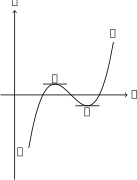
\includegraphics[width=0.4\linewidth]{fy-B-lectnotes_files/figure-latex/08-turning-points-1} 

}

\caption{turning points}\label{fig:08-turning-points}
\end{figure}

\slide

For the graph above:

\begin{slidesonly}

\begin{itemize}
\tightlist
\item
  The slope from \(A\) to \(B\) is:
\item
  The slope at \(B\) is:
\item
  The slope from \(B\) to \(C\) is:
\item
  The slope at \(C\) is:
\item
  The slope from \(C\) to \(D\) is:
\end{itemize}

\end{slidesonly}

\begin{notslides}

\begin{itemize}
\tightlist
\item
  The slope from \(A\) to \(B\) is positive.
\item
  The slope at \(B\) is zero.
\item
  The slope from \(B\) to \(C\) is negative.
\item
  The slope at \(C\) is zero.
\item
  The slope from \(C\) to \(D\) is positive.
\end{itemize}

\end{notslides}

As \(x\) increases from just before \(B\) to just after, the slope of the graph changes from positive to negative. A point such as \(B\) is called a \textcolor{red}{\em maximum}\index{maximum} or \textcolor{red}{\em local maximum}\index{local maximum}. The word ``local'' means that this is not the ``global'' maximum \(y\) value of the whole curve, but is the maximum value in the region ``near \(B\)'', e.g.~between \(A\) and \(C\).

As \(x\) increases from just before \(C\) to just after, the slope of the graph changes from negative to positive. A point such as \(C\) is known as a \textcolor{red}{\em minimum}\index{minimum} or \textcolor{red}{\em local minimum}\index{local minimum}.

Points such as \(B\) and \(C\) are also sometimes called \textcolor{red}{\em critical points}\index{critical points} or \textcolor{red}{\em stationary points}\index{stationary points} or \textcolor{red}{\em turning points}\index{turning points}. A function can have more than one maximum or minimum along its range of \(x\) values.
\slide

\subsection{Points of inflection}\label{points-of-inflection}

At any point on a graph where a maximum or minimum occurs, the gradient or rate of change of the curve is zero i.e.
\[
\frac{\mathrm{d} y}{\mathrm{d} x}=0.
\]
However, the converse is not necessarily true: the gradient may be zero, but the sign of the slope of the graph may not change. Such a point is called a \textcolor{red}{\em point of inflection}\index{point of inflection}.

\slide

\begin{figure}

{\centering 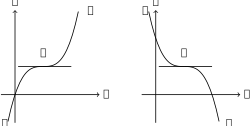
\includegraphics[width=0.6\linewidth]{fy-B-lectnotes_files/figure-latex/09-points-of-inflection-1} 

}

\caption{points of inflection}\label{fig:09-points-of-inflection}
\end{figure}

\begin{notslides}

In the left hand graph on Figure \ref{fig:09-points-of-inflection}, the slope is positive (strictly) between \(A\) and \(B\), and likewise between \(B\) and \(C\). At \(B\) it is zero.

Similarly on the right of Figure \ref{fig:09-points-of-inflection}:
the slope is negative between \(D\) and \(E\), between \(E\) and \(F\), and zero at \(E\).

\end{notslides}

\begin{slidesonly}

In the left hand graph on Figure \ref{fig:09-points-of-inflection}:

\begin{itemize}
\tightlist
\item
  between \(A\) and \(B\), the slope is:
\item
  at \(B\), the slope is:
\item
  between \(B\) and \(C\), the slope is:
\end{itemize}

\end{slidesonly}

The points \(B\) and \(E\) are both points of inflection.

\slide

We would like to be able to find out how many maxima, minima and points of inflection a curve has without having to plot the graph. We can do this by examining the derivatives of the function.

\begin{notslides}

Consider the curve of the function with the equation
\[
y = x^3-\frac 32x^2-18x+10.
\]
We know that at a stationary point, \(\mathrm{d}y/\mathrm{d} x=0\). So by finding \(\mathrm{d}y/\mathrm{d} x\) and setting it equal to zero, we can determine the \(x\) values of the stationary points as follows:
\begin{equation}
\frac{\mathrm{d} y}{\mathrm{d} x} = 3x^2-3x-18
\label{eq:3-1}
\end{equation}
Finding when \(\mathrm{d}y/\mathrm{d} x = 0\) leads to the (quadratic) equation
\begin{equation}
3x^2-3x-18=0.
\label{eq:3-2}
\end{equation}

\end{notslides}

\begin{slidesonly}

Consider the curve of the function with the equation
\[
y = x^3-\frac 32x^2-18x+10.
\]
We know that at a stationary point, \(\mathrm{d}y/\mathrm{d} x=0\). So by finding \(\mathrm{d}y/\mathrm{d} x\) and setting it equal to zero, we can determine the \(x\) values of the stationary points as follows:
\begin{equation}
\frac{\mathrm{d} y}{\mathrm{d} x} =\hbox to 5cm{}
\label{eq:3-1}
\end{equation}
Finding when \(\mathrm{d}y/\mathrm{d} x = 0\) leads to the equation
\begin{equation}
\label{eq:3-2}
\end{equation}

\end{slidesonly}

\slide

\begin{notslides}

We find that the quadratic equation \eqref{eq:3-2} has roots at \(x = 3\) and \(x = -2\). So now we know that there are two turning points, one at \(x = 3\) and one at \(x = -2\). We can find the \(y\) coordinates of these points by substituting each \(x\) value into equation \eqref{eq:3-1}. This gives \(y = -30.5\) when \(x = 3\) and \(y = 32\) when \(x = -2\).

We now know the coordinates of the turning points, but we do not know whether they are maxima, minima or points of inflection. We can often establish the type of turning point by considering the second derivative \(\mathrm{d}^{2}y/\mathrm{d} x^2\).

\end{notslides}

\begin{slidesonly}

Solving the equation \eqref{eq:3-2}:

\vfill

The stationary points are at:

\vfill

We find the corresponding \(y\) values by using equation \eqref{eq:3-1}. This yields:

\vfill

We now know the coordinates of the stationary points, but we do not know whether they are maxima, minima or points of inflection. We can often establish the type of turning point by considering the second derivative \(\mathrm{d}^{2}y/\mathrm{d} x^2\).

\end{slidesonly}

\slide

Consider a maximum of some function (generally).

\begin{figure}

{\centering 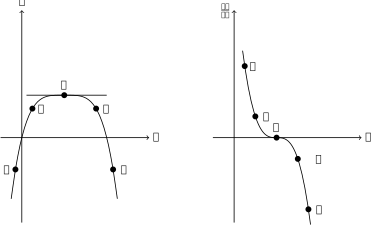
\includegraphics[width=0.8\linewidth]{fy-B-lectnotes_files/figure-latex/10-maximum-turning-point-1} 

}

\caption{maximum turning point}\label{fig:10-maximum-turning-point}
\end{figure}

\begin{notslides}

In the left hand graph on Figure \ref{fig:10-maximum-turning-point}, of the function \(y\), we have a local maximum. The gradient of the curve, \(\mathrm{d}y/\mathrm{d} x\), at point \(A\) will be a large positive value as the curve here is steeply sloped up from left to right. We can plot the value of the gradient at \(A\) on a graph (right hand graph above, of the function \(\mathrm{d}y/\mathrm{d} x\)). At \(B\) the slope of graph \(y\) is still positive, but less steep, so the gradient at \(B\), shown on the graph of \(\mathrm{d}y/\mathrm{d} x\) is still a positive value, but is smaller than at \(A\).

At \(C\) the gradient of graph \(y\) is zero. This is the point where the curve in graph of \(\mathrm{d}y/\mathrm{d} x\) crosses the \(x\) axis. At \(D\) the gradient of graph \(y\) is now negative, but not very steep, so on graph \(\mathrm{d}y/\mathrm{d} x\) the gradient at \(D\) is a small negative value. At \(E\) the gradient of graph \(y\) is steep and negative, so on graph \(\mathrm{d}y/\mathrm{d} x\) the point is marked as a large negative value.

Now consider the gradient of graph \(\mathrm{d}y/\mathrm{d} x\). Graph \(\mathrm{d}y/\mathrm{d} x\) is a plot of \(\mathrm{d}y/\mathrm{d} x\) against \(x\). The gradient of this graph is given by \(\mathrm{d}^{2}y/\mathrm{d} x^2\). We can see from the curve in that graph that the gradient of the curve is negative at all points. That is \(\mathrm{d}^{2}y/\mathrm{d} x^2<0\) for all \(x\) values close to the local maximum. Therefore if \(\mathrm{d}^{2}y/\mathrm{d} x^2\) is a negative number for the \(x\) value of the turning point, we can be sure the turning point is a maximum.
\slide

By a similar argument and considering the graphs below (Figure \ref{fig:11-minimum-turning-point}, we can show that for any turning point where, \(\mathrm{d}^{2}y/\mathrm{d} x^2>0\) we have a local minimum.

\end{notslides}

\begin{slidesonly}

Examine Figure \ref{fig:10-maximum-turning-point}.

\vfill

This leads to the following criterion:

If \(\mathrm{d}^{2}y/\mathrm{d} x^2\) \phantom{aaaaaaa} at a stationary point, then the stationary point is a local

\slide

Similarly with Figure \ref{fig:11-minimum-turning-point}.

\vfill

We get the other part of the criterion (called \textcolor{red}{\em second derivative criterion}\index{second derivative criterion}):

If \(\mathrm{d}^{2}y/\mathrm{d} x^2\) \phantom{aaaaaaa} at a stationary point, then the stationary point is a local

\end{slidesonly}

\begin{figure}

{\centering 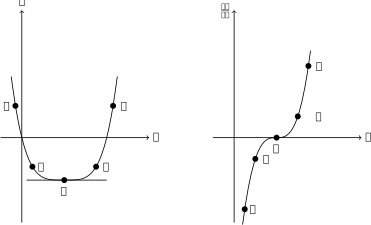
\includegraphics[width=0.8\linewidth]{fy-B-lectnotes_files/figure-latex/11-minimum-turning-point-1} 

}

\caption{minimum turning point}\label{fig:11-minimum-turning-point}
\end{figure}
\slide

Previously, we established that the curve \(y = x^3-\frac32 x^2-18x+10\) had turning points at \(x=3\) and \(x=-2\). We are now in a position to find out what kind of turning points each of these is.

\begin{notslides}

\[
\frac{\mathrm{d} y}{\mathrm{d} x} = 3x^2-3x-18\text{ therefore } \frac{\mathrm{d}^{2}y}{\mathrm{d} x^2} = 6x-3.
\]
When \(x = 3\), \(\mathrm{d}^{2}y/\mathrm{d} x^2=15 > 0\). So we deduce that the turning point at \(x=3\) is therefore a local minimum.

When \(x = -2\), \(\mathrm{d}^{2}y/\mathrm{d} x^2 = -15 < 0\) and so we deuce that the turning point at \(x = -2\) is therefore a local maximum.

\end{notslides}

\begin{slidesonly}

\[
\frac{\mathrm{d} y}{\mathrm{d} x} = 3x^2-3x-18\text{ therefore } \frac{\mathrm{d}^{2}y}{\mathrm{d} x^2} = 
\]

\begin{itemize}
\item
  When \(x = 3\), \(\mathrm{d}^{2}y/\mathrm{d} x^2=\)\\
  So the turning point at \(x=3\) is a local
\item
  When \(x = -2\), \(\mathrm{d}^{2}y/\mathrm{d} x^2=\)\\
  So the turning point at \(x=-2\) is a local
\end{itemize}

\end{slidesonly}

\slide

Note that the statement
\[
\text{When }x = 3, \frac{\mathrm{d}^{2}y}{\mathrm{d} x^2} = 15
\]
is often written as
\[
\left.\frac{\mathrm{d}^{2}y}{\mathrm{d} x^2}\right\vert_{x=3} = 15.
\]
Sometimes you can also see the notation
\[
\frac{\mathrm{d}^{2}y}{\mathrm{d} x^2}(3) = 15.
\]
Similarly we can write for the other statement that
\[
\left.\frac{\mathrm{d}^{2}y}{\mathrm{d} x^2}\right\vert_{x=-2} =
\frac{\mathrm{d}^{2}y}{\mathrm{d} x^2}(-2) = -15.
\]
\slide

There is a third possibility for the value of \(\mathrm{d}^{2}y/\mathrm{d} x^2\). It may be zero.

When \(\mathrm{d}^{2}y/\mathrm{d} x^2=0\), we may have a maximum, a minimum or a point of inflection at our turning point. We will need a further test to find out which.

\begin{notslides}

If we consider the points of inflection in Figure \ref{fig:09-points-of-inflection}, we can see that for the left-hand graph, the slope, \(\mathrm{d}y/\mathrm{d} x\) , is positive on both sides of the point of inflection. For the right hand graph the slope is negative on both sides of the point of inflection. For a maximum the slope always changes from positive to negative as x increases and for a minimum the slope always changes from negative to positive as \(x\) increases. This suggests a way of finding out what kind of turning point we have when \(\mathrm{d}^{2}y/\mathrm{d} x^2\) turns out to be zero.

\end{notslides}

\begin{slidesonly}

Consider again the points of inflection in Figure \ref{fig:09-points-of-inflection}.

\vfill

Consider the maximum and minimum in Figures \ref{fig:10-maximum-turning-point} \ref{fig:11-minimum-turning-point}.

\vfill

What can we say about the sign of the derivative near the stationary points?

\end{slidesonly}

\slide

We can substitute an \(x\) value just smaller than the value at the turning point into our equation for \(\mathrm{d}y/\mathrm{d} x\) and find if \(\mathrm{d}y/\mathrm{d} x\) is positive or negative at this \(x\) value, then we can do the same for an \(x\) value just larger than the \(x\) value of the turning point and again determine the sign of the outcome.

\slide

Then the type of turning point can be established according to the following table:

\begin{longtable}[]{@{}
  >{\raggedright\arraybackslash}p{(\columnwidth - 6\tabcolsep) * \real{0.2353}}
  >{\raggedright\arraybackslash}p{(\columnwidth - 6\tabcolsep) * \real{0.2353}}
  >{\raggedright\arraybackslash}p{(\columnwidth - 6\tabcolsep) * \real{0.2353}}
  >{\raggedright\arraybackslash}p{(\columnwidth - 6\tabcolsep) * \real{0.2941}}@{}}
\toprule\noalign{}
\begin{minipage}[b]{\linewidth}\raggedright
slope before turning pt
\end{minipage} & \begin{minipage}[b]{\linewidth}\raggedright
slope at turning pt
\end{minipage} & \begin{minipage}[b]{\linewidth}\raggedright
slope after turning pt
\end{minipage} & \begin{minipage}[b]{\linewidth}\raggedright
type of pt
\end{minipage} \\
\midrule\noalign{}
\endhead
\bottomrule\noalign{}
\endlastfoot
positive & zero & negative & maximum \\
negative & zero & positive & minimum \\
positive & zero & positive & inflection \\
negative & zero & negative & inflection \\
\end{longtable}

\slide

\begin{example}
Find and identify the critical or turning points of the function \(y=x^3\).
\end{example}

\begin{solution}
For \(y=x^3, \mathrm{d}y/\mathrm{d} x = 3x^2\). At a turning point \(\mathrm{d}y/\mathrm{d} x=0\) and so \(3x^2=0\) and so there is a turning point of some kind at \(x=0\).

\(\mathrm{d}^{2}y/\mathrm{d} x^2=6x\) and so
\[
\left.\frac{\mathrm{d}^{2}y}{\mathrm{d} x^2}\right\vert_{x=0} = 0.
\]
Thus we cannot identify the type of turning point from the second derivative.
However, we can consider the first derivative.

For \(x=-0.1\) (just less than \(0\)) \(\mathrm{d}y/\mathrm{d} x = 3(-0.1)^2 = 0.03>0\).

For \(x = 0.1\) (just greater than \(0\)) \(\mathrm{d}y/\mathrm{d} x=3(0.1)^2 = 0.03>0\).

So from examining the table above we see that the critical point at \(x=0\) must be a point of inflection.
\end{solution}

\slide

\subsection{Points of inflection}\label{points-of-inflection-1}

The points of inflection we have considered so far are a special case where the gradient is zero at
some value of x. In fact any point where the curve changes from concave to convex is called a
point of inflection regardless of whether the gradient becomes zero or not.

\slide

Two points of this type
are shown in the graphs on Figure \ref{fig:12-points-of-inflection}.

\begin{figure}

{\centering 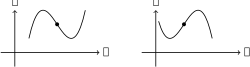
\includegraphics[width=0.6\linewidth]{fy-B-lectnotes_files/figure-latex/12-points-of-inflection-1} 

}

\caption{points of inflection}\label{fig:12-points-of-inflection}
\end{figure}

Here the graph changes from concave downwards to concave upwards as \(x\) increases in the first case and from concave upwards to concave downwards in the second case. In each case the marked point is a point of inflection. But the gradient is not zero at these points!

\slide

For points such as these \(\mathrm{d}y/\mathrm{d} x\) is not zero, but \(\mathrm{d}^{2}y/\mathrm{d} x^2\) always is. We can find the position of such points by finding where \(\mathrm{d}^{2}y/\mathrm{d} x^2\) is zero. We can decide which way they bend by considering \(\mathrm{d}y/\mathrm{d} x\) as for the previous point of inflection example.
\slide

\begin{example}
Find the \(x\) coordinates of all the maxima, minima and points of inflection for the curve
\[
y = 2x^3-9x^2+12x.
\]
\end{example}

\begin{solution}

For \(y = 2x^3-9x^2+12x\), \(\mathrm{d}y/\mathrm{d} x = 6x^2-18x+12\). When \(\mathrm{d}y/\mathrm{d} x=0\) then \(6x^2-18x+12=0\) and so \(x=2\) or \(x=1\).

Now \(\mathrm{d}^{2}y/\mathrm{d} x^2 = 12x-18\), so when \(x=2\), \(\mathrm{d}^{2}y/\mathrm{d} x^2>0\) and the point is a minimum.

When \(x=1\), \(\mathrm{d}^{2}y/\mathrm{d} x^2<0\) and the point is a maximum.

Also, \(\mathrm{d}^{2}y/\mathrm{d} x^2=0\) when \(x=1.5\) and so at \(x=1.5\) here is a point of inflection (but not of zero gradient).

From examining the value of \(\mathrm{d}y/\mathrm{d} x\) just before and just after \(x=1.5\) we find that the gradient is negative on both sides of the point of inflection and thus the curves slopes down from left to right.

\begin{figure}

{\centering 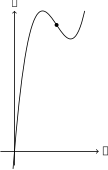
\includegraphics[width=0.4\linewidth]{fy-B-lectnotes_files/figure-latex/13-graph-of-2x3-9x2-12x-1} 

}

\caption{$y = 2x^3-9x^2+12x$}\label{fig:13-graph-of-2x3-9x2-12x}
\end{figure}

\end{solution}

\chapter*{Week 3 Exercises}\label{week-3-exercises}
\addcontentsline{toc}{chapter}{Week 3 Exercises}

\section{Sheet 8 Successive Differentiation}\label{sheet-8-successive-differentiation}

\subsection*{Exercise 1}\label{exercise-1-2}
\addcontentsline{toc}{subsection}{Exercise 1}

Determine the first four derivatives of the function
\[
y=x^3-4x^{3/2}.
\]
\slide

\subsection*{Exercise 2}\label{exercise-2-2}
\addcontentsline{toc}{subsection}{Exercise 2}

Show that \(y=4x\) is a solution to the differential equation
\[
2x^2\frac{d^2y}{dx^2}-x\frac{dy}{dx}+y=0.
\]

\slide

\subsection*{Exercise 3}\label{exercise-3-1}
\addcontentsline{toc}{subsection}{Exercise 3}

The displacement in metres for a particle moving along a line at time \(t\) seconds is given by the equation
\[
s=2t^2-10t+4.
\]
Determine the velocity at times of \(1.5\) and \(10\) seconds.

\slide

\subsection*{Exercise 4}\label{exercise-4-1}
\addcontentsline{toc}{subsection}{Exercise 4}

The velocity \(v\) of a particle moving along a line is given by
\[
v=-3t^2+18t+3
\]
where \(t\) is measured in seconds and \(v\) in metres per second. Determine the acceleration after \(2s\) and \(4s\).
\slide

\subsection*{Exercise 5}\label{exercise-5}
\addcontentsline{toc}{subsection}{Exercise 5}

The displacement of a body, measured in meters, from a reference point after time \(t\) seconds is given by
\[
s=4t^2-3t+2.
\]
Show that the acceleration of the body is constant at \(8ms^{-2}\) and that the velocity is zero after \(375ms\) (i.e.~after \(375\) milliseconds have elapsed).
\slide

\subsection*{Exercise 6}\label{exercise-6}
\addcontentsline{toc}{subsection}{Exercise 6}

The equation of motion of a particle is given by
\[
s=3+5t-6t^2
\]
where \(s\) is the displacement in metres and \(t\) is the time in seconds.

\begin{enumerate}
\def\labelenumi{\alph{enumi}.}
\tightlist
\item
  Determine its position, velocity and acceleration after a time of \(4s\).
\item
  Show that after \(415.6\overline{6}ms\) the body is momentarily at rest.
\end{enumerate}

{[}Solutions:
\textbf{1.} \(dy/dx=3x^2-6x^{1/2}\), \(d^2y/dx^2=6x-3x^{-1/2}\), \(d^3y/dx^3=6+3x^{-3/2}/2\), \(d^4y/dx^4=-9x^{-5/2}/4\);
\textbf{2.} \(dy/dx=4\), \(d^2y/dx^2=0\);
\textbf{3.} \(v(1.5) = -4m/s\), \(v(10) = 30m/s\);
\textbf{4.} \(a(2) = 6m/s^2\), \(a(4) = -6\ m/s^2\);
\textbf{5.} \(v=8t-3\), \(a=8\), \(v(0.375)=0m/s\);
\textbf{6.} \(v = -12t+5\), \(a=-12\), \(s(4) = -73m\), \(v(4)=-43m/s\), \(a(4)=-12m/s^2\), \(v(0.4166\overline{6})=0m/s\);{]}
\slide

\section{Sheet 8B More Examples of Successive Differentiation}\label{sheet-8b-more-examples-of-successive-differentiation}

\subsection*{Exercise 1}\label{exercise-1-3}
\addcontentsline{toc}{subsection}{Exercise 1}

If \(y(t) = a + bt^2 + ct^4\); where \(a\) and \(b\) are constants, find \(dy/dt\) and \(d^2y/dt^2\).

\slide

\subsection*{Exercise 2}\label{exercise-2-3}
\addcontentsline{toc}{subsection}{Exercise 2}

If \(y(t) = at -\frac 12gt^2\), where \(a\) and \(g\) are constants find \(dy/dt\) and \(d^2y/dt^2\).

\slide

\subsection*{Exercise 3}\label{exercise-3-2}
\addcontentsline{toc}{subsection}{Exercise 3}

If a body moves according to the law \(s = 12 - 4.5t + 6.2t^2\), find its velocity in metres when \(t = 4\) seconds. What can you say about the variation of the acceleration with time?

\slide

\subsection*{Exercise 4}\label{exercise-4-2}
\addcontentsline{toc}{subsection}{Exercise 4}

The angle \(\theta\) in radians turned through by a revolving wheel is connected by the time \(t\) (in seconds) that has elapsed since starting by the law
\[
\theta = 2.1 - 3.2t + 4.8t^2.
\]
Find the angular velocity (in radians per second) of that wheel when \(1.5\) seconds have elapsed. Find also its angular acceleration.

\slide

\subsection*{Exercise 5}\label{exercise-5-1}
\addcontentsline{toc}{subsection}{Exercise 5}

A slider moves so that, during the first part of its motion, its distance \(s\) (in metres) from its starting point is given by the expression
\[
s = 6.8t^3 - 10.8t
\]
\(t\) being in seconds. Find the expression for the velocity and acceleration at any time; and hence find the velocity and acceleration after \(3\) seconds.

\slide

\subsection*{Exercise 6}\label{exercise-6-1}
\addcontentsline{toc}{subsection}{Exercise 6}

The motion of a rising balloon is such that its height \(h\) in miles is given at any instant by the expression
\[
h = 05+ \frac1{10}\sqrt[3]{t-125}
\]
\(t\) being in seconds. Find an expression for the velocity and acceleration at any time. Draw curves to show the variation of height, velocity and acceleration during the first ten minutes of the ascent.

\slide

\subsection*{Exercise 7}\label{exercise-7}
\addcontentsline{toc}{subsection}{Exercise 7}

A body moves in such a way that the space described in the time \(t\) from starting is given by \(s = t^n\), where \(n\) is a constant. Find the value of \(n\) when the velocity is doubled from the 5th to the 10th second; find it also when the velocity is numerically equal to the acceleration at the end of the 10th second.

{[}Solutions:
\textbf{1.} \(dy/dt=2bt+4ct^3\), \(d^2y/dt^2=2b+12ct^2\);
\textbf{2.} \(dy/dt=a-gt\), \(d^2y/dt^2=-g\);
\textbf{3.} \(v=12.4t-4.5\), \(v(4)=45.1m/s\), \(a=12.4ms^{-2}\);
\textbf{4.} \(d\theta/dt(1.5)=11.2rad/s\), \(d^2\theta/dt^2 = 9.6rad/s^2\);
\textbf{5.} \(v=20.4t^2-10.8\), \(a=40.8t\), \(v(3)=172.8m/s\), \(a(3)=122.4m/s^2\);
\textbf{6.} \(v=(t-125)^{-2/3}/30\), \(a=-(t-125)^{-5/3}/45\);
\textbf{7.} \(n=2\), \(n=11\);{]}

\slide

\section{Sheet 9 Maxima, minima and points of inflexion}\label{sheet-9-maxima-minima-and-points-of-inflexion}

For each of the functions given below determine the \(x\) and \(y\) coordinates of any maxima, minima or points of inflexion. Find the coordinates of the points where the curves cross the \(x\) and \(y\) axes. Using all this information, sketch the graph of the function.

\begin{enumerate}
\def\labelenumi{\arabic{enumi}.}
\tightlist
\item
  \(y=x^2-4x+4\),
\item
  \(y=-2x^2+4x-5\),
\item
  \(y=x^2-x-12\),
\item
  \(y=2x^3-9x^2+12x+4\),
\item
  \(y=x^3+2x^2-1\),
\item
  \(y=x^3+6x^2-15x+3\),
\item
  \(y=x^3-9x^2+24x-7\),
\item
  \(y=x^4-8x^2\).
\end{enumerate}

{[}Solutions:
\textbf{1.} minimum at \((2,0)\);
\textbf{2.} maximum at \((1,-3)\), passes through \((0,-5)\);
\textbf{3.} minimum at \((0.5,-12.25)\), passes through \((0,-12), (-3,0), (4,0)\);
\textbf{4.} maximum at \((1,9)\), minimum at \((2,8)\), point of inflection at \((1.5,8.5)\), passes through \((0,4), (-0.274,0)\);
\textbf{5.} minimum at \((0,-1)\), maximum at \((-4/3,5/27)\), point of inflection at \((-2/3,-11/27)\), passes through \((0,-1), (-1.618,0), (-1,0), (0.618,0)\);
\textbf{6.} local maximum at \((-5,103)\), minimum at \((1,-5)\), point of inflection at \((-2,49)\), passes through \((0,3), (-7.937,0), (0.22,0), (1.717,0)\);
\textbf{7.} maximum at \((2,13)\), minimum at \((4,9)\), point of inflection at \((3,11)\), passes through \((0,-7), (0.331,0)\);
\textbf{8.} maximum at \((0,0)\), minimum at \((-2,-16)\), minimum at \((2,-16)\), points of inflection at \((-\sqrt{4/3},-80/9)\) and \((\sqrt{4/3},-80/9)\), passes through \((0,0), (-2\sqrt{2},0), (2\sqrt{2},0)\);{]}

\chapter{Week 4}\label{week-four}

We complete the content of the last `section' by learning about curve sketching before looking at specific problems from the world of Engineering relating to the computation of Maxima and Minima. Finally we look at implicit differentiation, parametric differentiation and logarithmic differentiation.

\slide

\section{Curve Sketching}\label{curve-sketching}

Given a function \(y=f(x)\) representing a curve in the plane, we wish to examine the function and its derivative(s) so as to be able to (roughly) sketch the graph of the function.

\begin{example}
Sketch the graph of the function
\[
y = x^2+3x-2.
\]
\end{example}

We collect the following information

\begin{enumerate}
\def\labelenumi{\arabic{enumi}.}
\tightlist
\item
  \(x\)-intercepts -- when \(y=0\);
\item
  \(y\)-intercept -- when \(x = 0\);
\item
  critical points and their classification -- from \(\mathrm{d}y/\mathrm{d} x, \mathrm{d}^2y/\mathrm{d}x^2\);
\item
  points of inflection;
\item
  asymptotes.
\end{enumerate}

\slide

\textbf{\emph{\(x\)-intercepts (of \(y = x^2+3x-2\))}}

Put \(y=0\) and solve for \(x\).

\begin{notslides}

\begin{align*}
x^2+3x-2 &= 0\\
x &= \frac{-3\pm\sqrt{3^2-4(-2)}}{2}\\
&=\frac{-3\pm\sqrt{17}}{2}
\end{align*}

\end{notslides}

\begin{slidesonly}

\vfill

\end{slidesonly}

\begin{notslides}

So the curve passes through the points \(((-3-\sqrt{17})/2,0)\) and \(((-3+\sqrt{17})/2,0)\).

\end{notslides}

\begin{slidesonly}

So the curve passes through the points:

\end{slidesonly}

\slide

\textbf{\emph{\(y\)-intercept (of \(y = x^2+3x-2\))}}

\begin{notslides}

Put \(x=0\) to find \(y(0) = 0^2+3\times0-2 = -2\).

So the curve passes through the point: \((0,-2)\).

\end{notslides}

\begin{slidesonly}

Put \(x=0\) to find:
\vfill
So the curve passes through the point:

\end{slidesonly}

\slide

\textbf{\emph{critical points (of \(y = x^2+3x-2\))}}

\begin{notslides}

\begin{align*}
\frac{\mathrm{d} y}{\mathrm{d} x} &= 2x+3 = 0 \Rightarrow x = -\frac{3}{2}\\
y(-\frac32) &= \left(-\frac32\right)^2 +3\left(-\frac 32\right) - 2 = -\frac{17}4\\
\frac{d^2y}{\mathrm{d} x^2} &= 2>0\Rightarrow x=-\frac 32\text{ is a local minimum}.
\end{align*}

\end{notslides}

\begin{slidesonly}

Find zeroes of the derivative\ldots{}
\vfill
So the curve passes through the point:

where it has a local

\end{slidesonly}

\slide

\textbf{\emph{points of inflection (of \(y = x^2+3x-2\))}}

\begin{notslides}

Since \(\mathrm{d}^2y/\mathrm{d}x^2 = 2\ne0\), there are no points of inflection
and the curve is always concave up.

\end{notslides}

\begin{slidesonly}

Since \(\mathrm{d}^2y/\mathrm{d}x^2 =\)

there are \phantom{nonono} points of inflection, and the curve is:
\vfill

\end{slidesonly}

Sketch on Figure \ref{fig:14-graph-x2-3x-2}.

\begin{figure}

{\centering 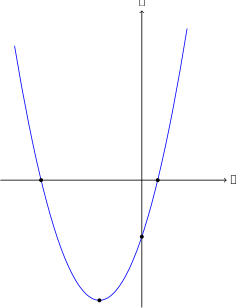
\includegraphics[width=0.4\linewidth]{fy-B-lectnotes_files/figure-latex/14-graph-x2-3x-2-1} 

}

\caption{$f(x)=x^2+3x-2$}\label{fig:14-graph-x2-3x-2}
\end{figure}
\slide

\begin{example}
Sketch the graph of the function
\[
y = x^3+2x+3.
\]
\end{example}

\textbf{\emph{\(x\)-intercepts (of \(y = x^3+2x+3\))}}

\begin{notslides}

Put \(y=0\) and solve for \(x\).
\[
x^3+2x+3 = 0.
\]
Notice that when \(x=-1\) then \(y=0\) and so \(x+1\) is a factor of \(y\). We can then find the other factor and see that
\[
y = (x+1)(x^2-x+3).
\]
The second factor \(x^2-x+3\) then has roots
\[
x = \frac{1\pm\sqrt{1-4\times3}}{2}
\]
which is not real and so there are no other \(x\)-intercepts, except \(x=-1\).

Hence the curve passes through \((-1,0)\).

\end{notslides}

\slide

\textbf{\emph{\(y\)-intercept (of \(y = x^3+2x+3\))}}

\begin{notslides}

Put \(x=0\) to find \(y(0) = 0^3+2\times0+3 = 3\).

So the curve passes through the point \((0,3)\).

\end{notslides}

\begin{slidesonly}

\end{slidesonly}

\slide

\textbf{\emph{critical points (of \(y = x^3+2x+3\))}}

\begin{notslides}

\[
\frac{\mathrm{d} y}{\mathrm{d} x} = 3x^2+2 = 0 \Rightarrow x^2 = -\frac{2}{3}.
\]
This has no real solutions and so there are no critical points.

\end{notslides}

\slide

\textbf{\emph{points of inflection (of \(y = x^3+2x+3\))}}

\begin{notslides}

Since \(\mathrm{d}^2y/\mathrm{d} x^2 = 6x\) then \((0,3)\) is a point of
inflection.
When \(x < 0\), \(\mathrm{d}^2y/\mathrm{d} x^2<0\) and so the curve is
concave down here, while if \(x>0\) then \(\mathrm{d}^2y/\mathrm{d} x^2>0\) and the
curve is concave up here.

\end{notslides}

\begin{slidesonly}

\vfill

\end{slidesonly}

Sketch on Figure \ref{fig:15-graph-x3-2x-3}.

\begin{figure}

{\centering 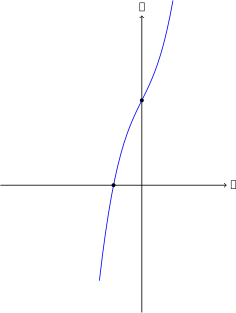
\includegraphics[width=0.4\linewidth]{fy-B-lectnotes_files/figure-latex/15-graph-x3-2x-3-1} 

}

\caption{$f(x)=x^3+2x+3$}\label{fig:15-graph-x3-2x-3}
\end{figure}
\slide

\begin{example}
Sketch the graph of the curve
\[
y = \frac{1}{x+1}.
\]
\end{example}

\textbf{\emph{\(x\)-intercepts (of \(1/(x+1)\))}}

\begin{notslides}

Put \(y=1/(x+1) = 0\) we see that there are no solutions and so the curve does not cross the \(x\)-axis.

\end{notslides}

\textbf{\emph{\(y\)-intercept (of \(1/(x+1)\))}}

\begin{notslides}

Put \(x=0\) to find \(y(0) = 1/(0+1) = 1\) and so the curve passes through the point \((0,1)\).

\end{notslides}

\slide

\textbf{\emph{critical points (of \(1/(x+1)\))}}

\begin{notslides}

\begin{align*}
y&=\frac1{x+1} = (x+1)^{-1}\\
\frac{\mathrm{d} y}{\mathrm{d} x} &= -(x+1)^{-2} = -\frac1{(x+1)^2}.
\end{align*}
This has no real solutions and so there are no critical points.

\end{notslides}

\slide

\textbf{\emph{points of inflection (of \(1/(x+1)\))}}

\begin{notslides}

\[
\frac{d^2y}{\mathrm{d} x^2} = -(-2)(x+1)^{-3} = \frac2{(x+1)^3}.
\]
This also has no solutions and so there are no points of inflection. Notice however that for \(x < -1\), \(\mathrm{d}^2y/\mathrm{d} x^2<0\) and so the function is concave down, while if \(x>-1\) then \(\mathrm{d}^2y/\mathrm{d} x^2 >0\) and so the function is concave up.

\end{notslides}

\begin{slidesonly}

\vfill (note: concave up/down)

\end{slidesonly}

\slide

\textbf{\emph{asymptotes}}

An \textcolor{red}{\em asymptote}\index{asymptote} of a curve is a line such that the distance between the curve and the line approaches zero as one or both of the \(x\) or \(y\) coordinates tends to infinity.

\slide

\textbf{\emph{asymptotes (of \(1/(x+1)\))}}

Notice that the given function is not actually defined at the point \(x=-1\) but that as \(x\to-1\) then \(y\to\pm\infty\). In fact if we approach the value of \(x=-1\) ``\textbf{from above}'' (i.e.~we start with \(x > -1\) and reduce its value to approach \(-1\)) then it is always the case that \(y>0\) and so \(y\to+\infty\) in this case. On the other hand if we approach \(x=-1\) ``\textbf{from below}'' (i.e.~start with \(x<-1\) and increase its value to approach \(-1\)) then it is always the case that \(y<0\) and so \(y\to-\infty\) in this case.

So the line \(x=-1\) is a \textcolor{red}{\em vertical asymptote}\index{vertical asymptote}.

\slide

There is also a \textcolor{red}{\em horizontal asymptote}\index{horizontal asymptote}. Notice that as \(x\to+\infty\) then \(y\to 0\) (from above), and as \(x\to-\infty\) then \(y\to0\) (from below). So the line \(y=0\) is a horizontal asymptote.

\begin{slidesonly}

\vfill

\end{slidesonly}

Sketch on Figure \ref{fig:16-graph-1-x-1}.

\begin{figure}

{\centering 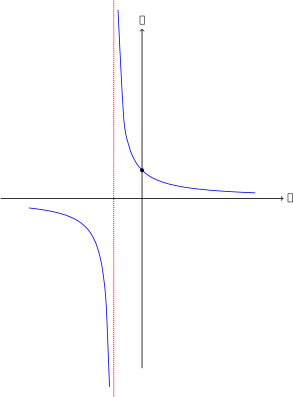
\includegraphics[width=0.4\linewidth]{fy-B-lectnotes_files/figure-latex/16-graph-1-x-1-1} 

}

\caption{$f(x)=1/(x+1)$}\label{fig:16-graph-1-x-1}
\end{figure}

\slide

\section{Engineering Problems with Max/Min}\label{engineering-problems-with-maxmin}

Maxima and minima may be used in engineering to solve problems such as finding the minimum surface area required to make an object with a fixed volume.

All such problems are solved by forming an equation for the quantity to be minimised (or maximised), i.e.~the surface area in the example above, and then using the first and second derivatives of the equation to find the minimum (or maximum) values. However, some intuition is often required to decide how the equation should be formed from the available information.

\slide

\begin{example}
Metal boxes are to be made from sheets of steel 800 mm long by 400 mm wide, by cutting squares from the corners and bending the sides. Determine the size of the square to be cut from a sheet such that the volume of the box is maximum.
\end{example}

It is usually helpful to begin by drawing a diagram (Figure \ref{fig:17-maximum-volume}).

\begin{figure}

{\centering 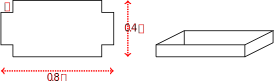
\includegraphics[width=0.7\linewidth]{fy-B-lectnotes_files/figure-latex/17-maximum-volume-1} 

}

\caption{maximum-volume}\label{fig:17-maximum-volume}
\end{figure}

Let \(x\) be the length in metres of side of the square to be cut.

The volume of the box
\[
V = \text{length}\times\text{breadth}\times\text{depth}\tag{1}
\]
Equation (1) is the equation we want to maximise, but we need to put the equation in terms of a single variable before we can differentiate.

\begin{notslides}

In terms of \(x\),
\[
\text{length} = 0.8 - 2x,\; \text{breadth} = 0.4 - 2x,\;\text{depth} = x
\]
So
\[
V = (0.8 - 2x)(0.4 - 2x)x = (0.32 - 2.4x + 4x^2)x = 4x^3 - 2.4x^2 + 0.32x
\]
Then
\[
\frac{\mathrm{d}V}{\mathrm{d} x} = 12x^2 - 4.8x + 0.32
\]
Maximum and minimum values occur when \(\mathrm{d}V/\mathrm{d}x  = 0\).
That is, when \(12x^2 - 4.8x + 0.32= 0\).

Solving \(12x^2 - 4.8x + 0.32= 0\) for \(x\) using the quadratic formula gives:
\[
 x \approx 0.316\text{ and }x \approx 0.085\,\,(3\text{ d.p.}).
\]
Now we need to find which value of \(x\) gives the maximum volume.
\begin{align*}
\frac{\mathrm{d}^2 V}{\mathrm{d} x^2} &= 24x - 4.8\\
\left.\frac{\mathrm{d}^2 V}{\mathrm{d} x^2}\right\vert_{x=0.316} &= 2.784\\
\left.\frac{\mathrm{d}^2 V}{\mathrm{d} x^2}\right\vert_{x=0.085} &= -2.772
\end{align*}

So \(x=0.316\) gives a positive value for \(d^2V/dx^2\) and so represents the minimum volume,

and \(x=0.085\) gives a negative value for \(d^2V/dx^2\) and so represents the maximum volume.

For maximum volume, the square to be cut out must have sides of \(0.085 m\), i.e.~\(85 mm\).

\end{notslides}

\begin{slidesonly}

In terms of \(x\),
\begin{align*}
\text{length} &=\\
\text{breadth} &=\\
\text{depth} &=\phantom{aklsdhflakjshdfklasdf}
\end{align*}
So \(V=\)

\slide

Recall: \(V(x)=4x^3 - 2.4x^2 + 0.32x\).

So \(\frac{d\mathrm{V}}{\mathrm{d} x} =\)

Maximum and minimum values occur when \(\mathrm{d}V/\mathrm{d}x  = 0\).

Thus:

\slide

Now we need to find which value of \(x\) gives the maximum volume.
\begin{align*}
\frac{\mathrm{d}^2 V}{\mathrm{d} x^2} &= \\
\left.\frac{\mathrm{d}^2 V}{\mathrm{d} x^2}\right\vert_{x=0.316} &=\\
\left.\frac{\mathrm{d}^2 V}{\mathrm{d} x^2}\right\vert_{x=0.085} &=
\end{align*}

So \(x=0.316\) gives

and \(x=0.085\) gives

For maximum volume, the square to be cut out must have sides of:

\slide

\end{slidesonly}

\begin{example}
A beam which is built into a wall at one end is simply supported by a force of 75 kN at the other end. The beam is loaded as shown below and the mass of the beam produces a force of 30kN/m. The beam is 4 m long, and the bending moment \(M\) at any distance \(x\) from the simply supported end is given by
\[
M = 75x-20(x-1.25)-30x\frac{x}{2}.
\]
Determine the position of the maximum bending moment and its magnitude. (Figure \ref{fig:18-maximum-bending-moment})
\end{example}

\begin{figure}

{\centering 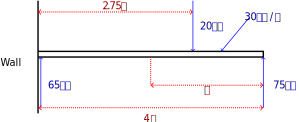
\includegraphics[width=0.65\linewidth]{fy-B-lectnotes_files/figure-latex/18-maximum-bending-moment-1} 

}

\caption{maximum bending moment}\label{fig:18-maximum-bending-moment}
\end{figure}
\slide

\begin{notslides}

\begin{align*}
M &= 75x - 20(x-1.25) - 30x\frac{x}{2},\\
\frac{\mathrm{d}M}{\mathrm{d} x} &= 75-20-30x = 55 - 30x.
\end{align*}
For a turning point, \(\mathrm{d}M/\mathrm{d}x=0\), so \(55 - 30x = 0\) and \(x = 1.83 m\).

\(\mathrm{d}^2M/\mathrm{d}x^2 = -30\), which is always negative, so the turning point is a maximum.

The bending moment \(M\) when \(x = 1.83\) is
\[
M = 75\times1.83 - 20(1.83 - 1.25) - \frac{30\times1.83^2}{2},
\]
or \(M = 75\ kNm\).

The maximum bending moment occurs at \(1.83 m\) from the simply supported end and has a value of \(75\ kNm\).

\end{notslides}

\begin{slidesonly}

\begin{align*}
M &= \phantom{75x - 20(x-1.25) - 30x\frac{x}{2}}\\
\frac{\mathrm{d}M}{\mathrm{d} x} &= 
\end{align*}
For a turning point, \(\mathrm{d}M/\mathrm{d}x=0\), so

\vfill

\(\frac{\mathrm{d}^2M}{\mathrm{d}x^2}\Big|_{x=\phantom{asdfasdf}} =\)

so the turning point is a

\slide

The bending moment \(M\) when \(x = 1.83\), is

\(M=\)

\vfill

Summary: The maximum bending moment occurs at \(1.83m\) from the simply supported end and has a value of:
\slide

\end{slidesonly}

\begin{example}

Given a cylindical can with surface area \(S=100\ m^2\), height \(h\) and radius \(r\) (see Figure \ref{fig:19-maximum-volume}),

\begin{enumerate}
\def\labelenumi{\arabic{enumi}.}
\tightlist
\item
  prove that the volume \(V = 50r-\pi r^3\);
\item
  find the value of \(r\) that maximises the volume.
\end{enumerate}

\end{example}

\begin{figure}

{\centering 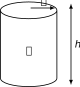
\includegraphics[width=0.25\linewidth]{fy-B-lectnotes_files/figure-latex/19-maximum-volume-1} 

}

\caption{maximum volume}\label{fig:19-maximum-volume}
\end{figure}
\slide

\begin{notslides}

Let \(A=\pi r^2\) be the surface area of the top of the can.

Notice that \(V = Ah = \pi r^2h\). So
\[
\begin{array}{rl}
S&=2A + \text{area of sides}\\
&=2\pi r^2 + 2\pi rh = 100\\
\end{array}
\]
\[
h=\frac{100-2\pi r^2}{2\pi r}=\frac{50-\pi r^2}{\pi r}
\]
\[
V=\pi r^2\left(\frac{50-\pi r^2}{\pi r}\right) = 50r -\pi r^3
\]
We need to find the critical points and so we find \(\mathrm{d}V/\mathrm{d} r\) and equate to 0.
\[
\frac{\mathrm{d} V}{\mathrm{d} r} = 50-3\pi r^2 = 0\text{ giving }r = \sqrt{\frac{50}{3\pi}}.
\]
Now
\[
\frac{\mathrm{d}^2 V}{\mathrm{d}r^2} = -6\pi r\;\text{ and so }\;\left.\frac{\mathrm{d}^2 V}{\mathrm{d}r^2}\right\vert_{r=\sqrt{50/3\pi}} = -6\pi\sqrt{\frac{50}{3\pi}}<0.
\]
By the 2nd derivative test we see that \(r=\sqrt{50/3\pi}\) is a local maximum.

\end{notslides}

\begin{slidesonly}

We have: \(A=\)
\vfill
\(100m^2=S=\)
\vfill
\(h=\)
\vfill
\(V=\)
\vfill
\slide
Recall \(V=50r-\pi r^3\).

We need to find the critical points and so we find \(\mathrm{d}V/\mathrm{d} r\) and equate to 0.

\(\dfrac{\mathrm{d} V}{\mathrm{d} r} =\)

\vfill

The critical point is \(r=\)

\vfill

\(\dfrac{\mathrm{d}^2 V}{\mathrm{d}r^2} =\)

\vfill

\(\left.\dfrac{\mathrm{d}^2 V}{\mathrm{d}r^2}\right\vert_{r=\phantom{adsfa}} =\)

and thus we have found a
\slide

\end{slidesonly}

\section{Further forms of differentiation}\label{further-forms-of-differentiation}

\subsection{Differentiation of implicit functions}\label{differentiation-of-implicit-functions}

An \textcolor{red}{\em implicit function}\index{implicit function} is one given by an equation (like the one below), rather than in a direct form \(y=\)(some expression with \(x\)). Here we consider \(y\) to depend on \(x\), and \(x\) to be an ``independent'' variable:
\[
y^2 + x^2 + 2xy + 2x = 0.
\]
Thus the whole expression is a function of \(x\) even though we don't have a formula for \(y\) in terms of \(x\).

We can still think of \(y=f(x)\), although we don't have a formula for \(f\). We do not need to ``solve the equation for \(y\)'' in order to differentiate, we can use the chain rule!

\slide

For example, to differentiate \(y^2\) with respect to \(x\) we write
\[
\frac{\mathrm{d}}{\mathrm{d} x}(y^2) = \frac{\mathrm{d}}{\mathrm{d} y}(y^2)\times\frac{\mathrm{d} y}{\mathrm{d} x}= 2y\frac{\mathrm{d} y}{\mathrm{d} x}.
\]
\slide
To differentiate \(2xy\) we note that if \(y=f(x)\) was known, this would be a product of two functions of \(x\), so using the product rule
\[
\frac{\mathrm{d}}{\mathrm{d} x}(2xy) = 2x\frac{\mathrm{d}}{\mathrm{d} x}(y)+2y\frac{\mathrm{d}}{\mathrm{d} x}(x) = 2x\frac{\mathrm{d} y}{\mathrm{d} x} + 2y.
\]
\slide
Hence if
\[
y^2 + x^2 + 2xy + 2x = 0
\]
then the derivative with respect to \(x\) is

\begin{notslides}

\[
2y\frac{\mathrm{d} y}{\mathrm{d} x} + 2x+2x\frac{\mathrm{d} y}{\mathrm{d} x} +2y+2 = 0.
\]
This may be rearranged so that
\begin{align*}
2y\frac{\mathrm{d} y}{\mathrm{d} x}+2x\frac{\mathrm{d} y}{\mathrm{d} x} &= -2x-2y-2\\
\frac{\mathrm{d} y}{\mathrm{d} x}(2y+2x) &= -2(x+y+1)\\
\frac{\mathrm{d} y}{\mathrm{d} x} &= \frac{-(x+y+1)}{x+y}.
\end{align*}

\end{notslides}

\begin{slidesonly}

\slide

This can be rearranged to get:

\end{slidesonly}

\slide

\begin{example}
Differentiate with respect to \(x\), \(10x^2 + 12xy + 10y^2 = 1\) where \(y = f(x)\). Hence find the gradient of the tangent(s) to the curve when \(x=0.2\).
\end{example}

\begin{figure}

{\centering 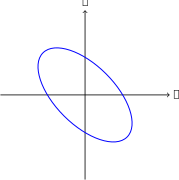
\includegraphics[width=0.5\linewidth]{fy-B-lectnotes_files/figure-latex/20-ellipse-1} 

}

\caption{ellipse $10x^2 + 12xy + 10y^2 = 1$}\label{fig:20-ellipse}
\end{figure}

\begin{solution}
This is actually the equation of an ellipse (Figure \ref{fig:20-ellipse}).

\begin{align*}
10x^2 + 12xy + 10y^2 &= 1\\
20x+12x\frac{\mathrm{d} y}{\mathrm{d} x}+12y+20y\frac{\mathrm{d} y}{\mathrm{d} x} &=0\\
\frac{\mathrm{d} y}{\mathrm{d} x} = \frac{-20x-12y}{12x+20y} &= -\frac{5x+3y}{3x+5y}.
\end{align*}

When \(x=0.2\) then
\[
10y^2+\frac{12}5y-\frac35=0\text{ and so }y = \frac{-\frac{12}5\pm\sqrt{\left(\frac{12}5\right)^2+4\times10\times\frac35}}{20} = 0.153\text{ and }-0.393
\]
So
\[
\left.\frac{\mathrm{d} y}{\mathrm{d} x}\right|_{x=0.153} = -\frac{5\times0.2+3\times 0.153}{3\times0.2+5\times0.153} = -1.069
\]
and
\[
\left.\frac{\mathrm{d} y}{\mathrm{d} x}\right|_{x=-0.393} = -\frac{5\times0.2-3\times 0.393}{3\times0.2-5\times0.393} = -0.091
\]
\end{solution}

\slide

\begin{slidesonly}

\phantom{a}
\slide

\end{slidesonly}

\subsection{Differentiation in parameters}\label{differentiation-in-parameters}

If a function is expressed in parametric form it is convenient to be able to differentiate it in this form rather than having to convert to Cartesian form first.

A function expressed in parametric form has a third variable e.g.
\[
y = f(t),\; x = g(t)
\]
where \(t\) is a parameter.

Now using the chain rule again
\[
\frac{\mathrm{d} y}{\mathrm{d} t} = \frac{\mathrm{d} y}{\mathrm{d} x}\times\frac{\mathrm{d} x}{\mathrm{d} t}\text{ and so }\frac{\mathrm{d} y}{\mathrm{d} x} = \frac{\mathrm{d} y}{\mathrm{d} t}/\frac{\mathrm{d} x}{\mathrm{d} t}.
\]
Thus if we can find \(\mathrm{d}y/\mathrm{d} t\) and \(\mathrm{d}x/\mathrm{d} t\) we can establish \(\mathrm{d}y/\mathrm{d} x\).

\slide

\begin{example}
A function is expressed in parametric form as \(y = 2t + t^2, x = t^2 - 1\), where \(t\) is a parameter. Find \(\mathrm{d}y/\mathrm{d} x\).
\end{example}

\begin{solution}
\begin{gather*}
\frac{\mathrm{d} y}{\mathrm{d} t} = 2+2t\\
\frac{\mathrm{d} x}{\mathrm{d} t} = 2t\\
\frac{\mathrm{d} y}{\mathrm{d} x} = \frac{\mathrm{d} y}{\mathrm{d} t}/\frac{\mathrm{d} x}{\mathrm{d} t} = \frac{2+2t}{2t} = \frac{1+t}{t}.
\end{gather*}
\end{solution}

\slide

\subsection{Logarithmic differentiation}\label{logarithmic-differentiation}

This is a convenient way to deal with the derivative of a product of quotient with more than two terms.

Consider
\[
y = \frac{(x-4)(x+5)}{(x+3)(x-2)}
\]
Taking logs of both sides gives

\begin{notslides}

\[
\ln(y) = \ln(x-4)+\ln(x+5)-\ln(x+3)-\ln(x-2)
\]

\end{notslides}

\begin{slidesonly}

\(\ln(y) =\)

\end{slidesonly}

\slide

\begin{slidesonly}

Recall: \(\ln(y) = \ln(x-4)+\ln(x+5)-\ln(x+3)-\ln(x-2)\).

\end{slidesonly}

Differentiating and treating \(\ln(y)\) as a function of a function gives

\begin{notslides}

\begin{align*}
\frac 1y\times\frac{\mathrm{d} y}{\mathrm{d} x} &= \frac{1}{x-4}+\frac{1}{x+5}-\frac{1}{x+3}-\frac{1}{x-2}\\
\frac{\mathrm{d} y}{\mathrm{d} x} &= y\times\left(\frac{1}{x-4}+\frac{1}{x+5}-\frac{1}{x+3}-\frac{1}{x-2}\right)\\
&= \left(\frac{1}{x-4}+\frac{1}{x+5}-\frac{1}{x+3}-\frac{1}{x-2}\right)\frac{(x-4)(x+5)}{(x+3)(x-2)}.
\end{align*}

\end{notslides}

\begin{slidesonly}

\slide

\end{slidesonly}

\begin{example}
Differentiate with respect to \(x\), \(y=x^x\).
\end{example}

\begin{solution}
\begin{align*}
\ln(y) &= x\ln(x)\\
\frac{1}{y}\times\frac{\mathrm{d} y}{\mathrm{d} x} &= \ln(x)+x\times\frac{1}{x} = \ln(x)+1\\
\frac{\mathrm{d} y}{\mathrm{d} x} &= y(\ln(x)+1) = x^x(\ln(x)+1).
\end{align*}
\end{solution}

\chapter*{Week 4 Exercises}\label{week-4-exercises}
\addcontentsline{toc}{chapter}{Week 4 Exercises}

\section{Sheet 10 - Curve Sketching using differentiation}\label{sheet-10---curve-sketching-using-differentiation}

For each of the given functions find the \(y-\)intercept, \(x-\)intercepts, local maxima, local minima
and points of inflection. Sketch the graph of the function clearly indicating these points.

\begin{enumerate}
\def\labelenumi{\arabic{enumi}.}
\tightlist
\item
  \(y=x^2+3x-2\).
\item
  \(y=x^3+2x+3\).
\item
  \(f(x)=x^4-6x^2\).
\item
  \(f(x)=x^5-5x^4\).
\item
  \(g(x)=\sin(x)\).
\item
  \(g(x)=\cos(x)\).
\item
  \(y=1/(x+1)\).
\item
  \(y=1/(x^2+1)\).
\item
  \(f(x)=e^x\).
\item
  \(h(x)=\ln(x)\).
\end{enumerate}

{[}Solutions: 1. \((0,-2), (-3.56,0), (0.56,0), (-3/2,-17,4)\) is a minimum; 2. \((0,3), (-1,0), (0,3)\) is point of inflection; 3. \((0,0), (0,0), (\pm\sqrt{6},0), (0,0)\) is a maximum, \((\pm\sqrt{3},-9)\) are minima, \((\pm 1,-5)\) are points of inflection; 4. \((0,0), (0,0), (5,0), (0,0)\) is a maximum, \((4,-256)\) is a minimum, \((0,0), (3,-162)\) are points of inflection; 5. \((0,0), (0,0), (\pi,0), (\pi/2,1)\) is a maximum, \((3\pi/2,-1)\) is a minimum; 6. \((0,1), (\pi/2,0), 3\pi/2,0), (0,1)\) is a maximum, \((\pi,-1)\) is a minimum; 7. \((0,1)\); 8. \((0,1), (0,1)\) is a maximum, \((\pm\sqrt{1/3},3/4)\) are points of inflection; 9. \((0,1)\); 10. \((1,0)\){]}
\slide

\section{Sheet 11 - Problems involving maxima \& minima}\label{sheet-11---problems-involving-maxima-minima}

\subsection*{Exercise 1}\label{exercise-1-4}
\addcontentsline{toc}{subsection}{Exercise 1}

A beam 3 m long whose weight is 2 kN, is simply supported at both ends and the bending moment at a distance \(x\ m\) from one end is given by
\[
m = 2(3x - x^2)\ kNm
\]
Prove that the bending moment is a maximum in the middle of the beam and calculate its value.

\slide

\subsection*{Exercise 2}\label{exercise-2-4}
\addcontentsline{toc}{subsection}{Exercise 2}

If \(150\ m\) of fencing is to be used to enclose three sides of a rectangular plot of land, whilst the remaining side is to be a river bank, determine the lengths of the sides such that the area enclosed will be a maximum.

\slide

\subsection*{Exercise 3}\label{exercise-3-3}
\addcontentsline{toc}{subsection}{Exercise 3}

A totally enclosed cylinder of radius \(r\), has a surface area of \(100 m^2\). Prove that the volume of the shape, \(V\), is given by \(V = 50r - \pi r^3\) and determine the value of \(r\) which maximize the volume.

\slide

\subsection*{Exercise 4}\label{exercise-4-3}
\addcontentsline{toc}{subsection}{Exercise 4}

Prove that a rectangle of fixed area has its minimum perimeter when it becomes a square.

\slide

\subsection*{Exercise 5}\label{exercise-5-2}
\addcontentsline{toc}{subsection}{Exercise 5}

An arch of a bridge is designed as a rectangle surmounted by a semicircle. If the area of the archway is \(100\ m^2\), determine the radius of the semicircle such that the perimeter of the edge has a minimum value.

\slide

\subsection*{Exercise 6}\label{exercise-6-2}
\addcontentsline{toc}{subsection}{Exercise 6}

Find the least area of metal required to make a cylindrical container from thin metal sheet in order that it might have a capacity of \(2000\pi\ cm^3\).

{[}Solutions: 1. \(3/2,18/4)\); 2. \(x=37.5, y = 75\); 3. \(r=\sqrt{50/(3\pi)}\); 5. \(r=\sqrt{100/(2+\pi/2)}\); 6. \(600\pi\){]}
\slide

\section{Sheet 11A - Logarithmic Differentiation}\label{sheet-11a---logarithmic-differentiation}

Use logarithmic differentiation to find \(dy/dx\) when

\begin{enumerate}
\def\labelenumi{\arabic{enumi}.}
\tightlist
\item
  \(y = (5x+2)(3x-7)\).
\item
  \(y = \frac{3x+5}{(x-3)(x+4)}\).
\item
  \(y = \frac{3x+5}{x^2+x-12}\).
\item
  \(y = \frac{x^2-12x+26}{(x-2)(x-3)(x-4)}\).
\item
  \(y = \frac{x+3}{(x+2)^2(x-1)}\).
\item
  \(y = \frac{7x^2+9x-1}{(3x-2)^4}\).
\item
  \(y = \frac{(x+2)^2(2x-5)}{(6x+5)^3(x^3+4)^2}\).
\item
  \(y = x^{\sin(x)}\).
\item
  \(y = x^x\).
\item
  \(y = a^x\).
\end{enumerate}

{[}Solutions: 1. \((5x+2)(3x-7)\left(5/(5x+2)+3/(3x-7)\right)\); 2. \((3x+5)/((x-3)(x+4))\left(3/(3x+5)-1/(x-3)-1/(x+4)\right)\); 3. \((3x+5)/(x^2+x-12)\left(3/(3x+5)-(2x+1)/(x^2+x-12)\right)\); 4. \((x^2-13x+26)/((x-2)(x-3)(x-4))\left((2x-13)/(x^2-13x+26)-1/(x-2)-1/(x-3)-1/(x-4)\right)\); 5. \((x+3)/((x+2)^2(x-1))\left(1/(x+3)-2/(x+2)-1/(x-1)\right)\); 6. \((7x^2+9x-1)/(3x-2)^4\left((14x+9)/(7x^2+9x-1)-12/(3x-12)\right)\); 7. \((x+2)^2(2x-5)/((6x+5)^3(x^3+4)^2)\left(2/(x+2)+1/(2x-5)-18/(6x+5)-6x^2/(x^3+4)\right)\); 8. \(x^{\sin(x)}\left(\cos(x)\ln(x)+\sin(x)/x\right)\); 9. \(x^x(\ln(x)+1)\); 10. \(a^x\ln(a)\){]}

\section{Sheet 11B - Further Differentiation}\label{sheet-11b---further-differentiation}

\subsection*{Exercise 1}\label{exercise-1-5}
\addcontentsline{toc}{subsection}{Exercise 1}

Differentiate the following implicit functions

\begin{enumerate}
\def\labelenumi{\roman{enumi}.}
\tightlist
\item
  \(x^2+y^2-5x-6y+8=0\);
\item
  \(3x^2+2xy+3y^2=0\);
\item
  \(x^3+y^3+8x^2y=25\).
\end{enumerate}

\slide

\subsection*{Exercise 2}\label{exercise-2-5}
\addcontentsline{toc}{subsection}{Exercise 2}

Find \(dy/dx\) for the following functions quoted in parametric form where \(t\) and \(\theta\) are parameters and \(a\) is a constant.

\begin{enumerate}
\def\labelenumi{\roman{enumi}.}
\tightlist
\item
  \(y=2at, x = at^2\);
\item
  \(y=t^2, x = 2t\);
\item
  \(y=3\cos(\theta)-\sin^3(\theta), x = \cos^3(\theta)\).
\end{enumerate}

\slide

\subsection*{Exercise 3}\label{exercise-3-4}
\addcontentsline{toc}{subsection}{Exercise 3}

Obtain \(dy/dx\) for each function by writing it in logarithmic form

\begin{enumerate}
\def\labelenumi{\roman{enumi}.}
\tightlist
\item
  \(y=\frac{x^2\sin(x)}{\cos(2x)}\);
\item
  \(y=x^5e^{3x}\tan(x)\);
\item
  \(y=\frac{(3x+2)\cos(2x)}{e^{2x}}\).
\end{enumerate}

{[}Solutions: 1(i) \((2y-6)dy/dx+2x-5=0\), (ii) \((2x+6y)dy/dx+6x+2y=0\), (iii) \((3y^2+8x^2)dy/dx+3x^2+16xy=0\); 2(i) \(dy/dx = 1/t\), (ii) \(dy/dx = t\), (iii) \(dy/dx = (1+\sin(\theta)\cos(\theta))/\cos^2(\theta)\); 3 (i) \(dy/dx=x^2\sin(x)/\cos(x)\left(2/x+\cos(x)/\sin(x)+2\sin(2x)/\cos(2x)\right)\), (ii) \(dy/dx = x^5e^{3x}\tan(x)\left(5/x+3+\sec^2(x)/\tan(x)\right)\), (iii) \(dy/dx = ((3x+2)\cos(2x))/e^{2x}\left(3/(3x+2)-2\sin(2x)/\cos(2x)-2\right)\){]}

\chapter{Week 5}\label{week-five}

We close ``differentiation'' by considering functions that have more than one variable, and differentiating with respect to either of them.

We then move on to look at the opposite process to differentiation, called integration. Given the derivative of a function, can we find a function that gave rise to that derivative?

\slide

\section{Partial Differentiation}\label{partial-differentiation}

If an expression is a function of two variables then it can be differentiated with respect to either of the variables.

For example, suppose
\[
z(x,y) = x^2+xy+y^2.
\]
If we fix the value of the variable \(y\) and consider this as a function of the variable \(x\) only.

\begin{notslides}

For example, if \(y=2\), then
\[
z(x,2) = x^2 + 2x + 4.
\]
We can differentiate this function with respect to \(x\) to get \(\mathrm{d}z(x,2)/\mathrm{d}x = 2x+2\).

Similarly, we can fix the value of the variable \(x\) and consider it as a function of \(y\) only. For example if \(x=-1\), then
\[
z(-1,y) = 1-y+y^2.
\]
T

\end{notslides}

\begin{slidesonly}

For example, if \(y=2\), then
\[
z(x,2) = \phantom{x^2 + 2x + 4.}
\]
We can differentiate this function with respect to \(x\) to get \(\mathrm{d}z(x,2)/\mathrm{d}x =\)

\slide

(Recall: \(z(x,y) = x^2+xy+y^2\).)

Similarly, we can fix the value of the variable \(x\) and consider it as a function of \(y\) only. For example if \(x=-1\), then
\[
z(-1,y) =
\]
The derivative of this with respect to \(y\) is then \(\mathrm{d}z(-1,y)/\mathrm{d}y =\)

\slide

\end{slidesonly}

\begin{notslides}

In general, if we think of \(y\) as being a fixed constant (not worrying about the actual value), then we can differentiate \(z\) with respect to \(x\). We use the following notation
\[
\frac{\partial z}{\partial x} = 2x+y.
\]
In the same way, thinking of \(x\) as being a fixed constant and differentiating with respect to \(y\) we write
\[
\frac{\partial z}{\partial y} = x + 2y.
\]

\end{notslides}

\begin{slidesonly}

(Recall: \(z(x,y) = x^2+xy+y^2\).)

In general, if we think of \(y\) as being a fixed constant (not worrying about the actual value), then we can differentiate \(z\) with respect to \(x\). We use the following notation
\[
\frac{\partial z}{\partial x} = \phantom{2x+y.}
\]
In the same way, thinking of \(x\) as being a fixed constant and differentiating with respect to \(y\) we write
\[
\frac{\partial z}{\partial y} = \phantom{x + 2y.}
\]

\slide

\end{slidesonly}

Consider the expression for the volume of a cylinder, \(V = \pi r^2h\) where \(r\) is the radius of the cylinder and \(h\) is its height. (Figure \ref{fig:21-cylinder})

\begin{figure}

{\centering 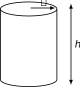
\includegraphics[width=0.25\linewidth]{fy-B-lectnotes_files/figure-latex/21-cylinder-1} 

}

\caption{cylinder}\label{fig:21-cylinder}
\end{figure}

\begin{notslides}

The two different ``derivatives'' are
\begin{align*}
\text{treating }h\text{ as a constant } \frac{\partial V}{\partial r} &= 2\pi rh\\
\text{treating }r\text{ as a constant } \frac{\partial V}{\partial h} &= \pi r^2
\end{align*}

\end{notslides}

\begin{slidesonly}

The two different ``derivatives'' are
\begin{align*}
\text{treating }h\text{ as a constant } \frac{\partial V}{\partial r} &= \phantom{2\pi rh}\\
\text{treating }r\text{ as a constant } \frac{\partial V}{\partial h} &= \phantom{\pi r^2}
\end{align*}
\slide

\end{slidesonly}

We use the symbol \(\partial\) in the derivatives above to indicate that there is more than one variable by which the expression may be differentiated and that we have chosen to treat any other variables as constants while differentiating.

The first type of derivative tells us how the volume would vary as the radius was varied for a cylinder of constant height. The second type of derivative tells us how the volume would vary as the height varied for a cylinder of constant radius.

When a function of more than one variable is differentiated with respect to one variable only, this process is called \textcolor{red}{\em partial differentiation}\index{partial differentiation}.

\slide

\begin{example}
From the function \(z=x^3y^2\), determine \(\partial z/\partial x\) and \(\partial z/\partial y\).
\end{example}

\begin{solution}
\[
\frac{\partial z}{\partial x} = 3x^2y^2,\;\frac{\partial z}{\partial y} = 2yx^3.
\]
\end{solution}

\slide

\begin{example}
From the function \(z=3x^5-5y^3+6\), determine \(\partial z/\partial x\) and \(\partial z/\partial y\).
\end{example}

\begin{solution}
\[
\frac{\partial z}{\partial x} = 15x^4,\;\frac{\partial z}{\partial y} = -15y^2.
\]
\end{solution}

\slide

\subsection{Successive partial derivatives}\label{successive-partial-derivatives}

If a second partial derivative is required and there are, say, two variables, then a second derivative may be made with each of these variables.

\begin{example}
Calculate all possible ``second partial derivatives'' of
\[
z=3x^2+2x^2y^2+3y^2.
\]
\end{example}

\begin{solution}
\[
\frac{\partial z}{\partial x} = 6x+4xy^2,\;\frac{\partial z}{\partial y} = 4x^2y+6y.
\]
So
\[
\frac{\partial}{\partial x}\left(\frac{\partial z}{\partial x}\right) = \frac{\partial^2 z}{\partial x^2} = 6+4y^2
\]
\[
\frac{\partial}{\partial y}\left(\frac{\partial z}{\partial y}\right) = \frac{\partial^2 z}{\partial y^2} = 6+4x^2
\]
\[
\frac{\partial}{\partial x}\left(\frac{\partial z}{\partial y}\right) = \frac{\partial^2 z}{\partial x\partial y} = 8xy
\]
\[
\frac{\partial}{\partial y}\left(\frac{\partial z}{\partial x}\right) = \frac{\partial^2 z}{\partial y\partial x} = 8xy
\]
\end{solution}

\begin{slidesonly}

\slide

(Recall: \(z=3x^2+2x^2y^2+3y^2\).)
\slide

\end{slidesonly}

\begin{example}
Calculate all possible ``second partial derivatives'' of
\[
z = x\cos(y)-y\cos(x)
\]
\end{example}

\begin{solution}
\[
\frac{\partial z}{\partial x} = \cos(y)+y\sin(x),\;\frac{\partial z}{\partial y} = -x\sin(y)-\cos(x).
\]
So
\[
\frac{\partial}{\partial x}\left(\frac{\partial z}{\partial x}\right) = \frac{\partial^2 z}{\partial x^2} = y\cos(x)
\]
\[
\frac{\partial}{\partial y}\left(\frac{\partial z}{\partial y}\right) = \frac{\partial^2 z}{\partial y^2} = -x\cos(y)
\]
\[
\frac{\partial}{\partial x}\left(\frac{\partial z}{\partial y}\right) = \frac{\partial^2 z}{\partial x\partial y} = -\sin(y)+\sin(x)
\]
\[
\frac{\partial}{\partial y}\left(\frac{\partial z}{\partial x}\right) = \frac{\partial^2 z}{\partial y\partial x} = -\sin(y)+\sin(x)
\]
\end{solution}

\slide

\section{Integration as the opposite of differentiation}\label{integration-as-the-opposite-of-differentiation}

Given a function \(f(x)\), we have seen the notion of the \textbf{inverse function}, that is a function \(g(x)\) such that \(f(g(x)) = x\) (or \(g(f(x))=x\); which one?). For example if \(f(x) = x^2\) (for \(x\geq0\)), then taking \(g(x) = \sqrt{x}\) (for \(x\geq0\)) indeed verifies \(f(g(x)) = (\sqrt{x})^2 = x\). The inverse `undoes' what the original function does.

Integration is the ``inverse'' of differentiation. That is, having been given the derivative of a function, we are asking; what was the original function that was differentiated to get that derivative? (\href{https://xkcd.com/2117/}{xkcd})

The symbol for integration is \(\displaystyle\int\), which is the Old English symbol for ``s''. The symbol is used to indicate that integration is a summation process. We shall see why later.

\slide

\subsection{Integration by rule}\label{integration-by-rule}

Suppose \(\mathrm{d}y/\mathrm{d} x = 2x\). Then the instruction ``integrate this function with respect to \(x\)'' is written
\[
\int 2x \,\mathrm{d}x
\]
We know that to get
\[
\frac{\mathrm{d}y}{\mathrm{d}x} = 2x
\]
we could have started with \(y = x^2\) so this is one possible solution.

\begin{notslides}

However, we could also have started with \(y = x^2 + 5\) or \(y = x^2 + 1\) or \(y = x^2 + 25\) or \(y = x^2 + 1245\).

\end{notslides}

\begin{slidesonly}

However, we could also have started with \(y =\)
\slide

\end{slidesonly}

We can't tell which because all information about the any constant value is lost when we differentiate. To make this clear we write
\[
\int 2x \,\mathrm{d}x = x^2 + c
\]
where ``\(c\)'' represents an arbitrary constant.

\slide

General rules for simple functions follow from the differentiation rules:

For differentiation, we had that if \(y = x^n\), then \(\mathrm{d}y/\mathrm{d} x= nx^{n-1}\).

Thus for integration, if \(\mathrm{d}y/\mathrm{d}x = x^n\) then \(y=\displaystyle\int x^n \,\mathrm{d}x = \frac{x^{n+1}}{n+1} + c\), if \(n \ne -1\).

After a function has been integrated, the result of integration may be checked by differentiating the answer.

\slide

Similarly as for derivatives, constants and \(\pm\) ``come out of the integral'':

\begin{itemize}
\tightlist
\item
  Summation Rule: \(\displaystyle\int(f(x)+g(x))\,\mathrm{d}x = \displaystyle\int f(x)\,\mathrm{d}x + \displaystyle\int g(x)\,\mathrm{d}x\).
\item
  Coefficient Rule: \(\displaystyle\int af(x)\,\mathrm{d}x = a\displaystyle\int f(x)\,\mathrm{d}x\).
\item
  Power Rule: \(\displaystyle\int x^n \,\mathrm{d}x = x^{n+1}/(n+1) + c\).
\end{itemize}

\slide

\begin{example}

Integrate the functions

\begin{enumerate}
\def\labelenumi{\arabic{enumi}.}
\tightlist
\item
  \(y=x^3\)
\item
  \(y=3x^2\)
\item
  \(y=6x-4\)
\item
  \(y=(8x^2-4x+5)/x^4\)
\item
  \(y=x^{3/5}(2x-\sqrt{x})\)
\end{enumerate}

\end{example}

\begin{solution}
\leavevmode

\begin{enumerate}
\def\labelenumi{\arabic{enumi}.}
\tightlist
\item
  \(\displaystyle\int x^3 \,\mathrm{d}x = x^4/4+c\),
\item
  \(\displaystyle\int 3x^2 \,\mathrm{d}x = 3x^3/3+c = x^3+c\),
\item
  \(\displaystyle\int(6x-4)\,\mathrm{d}x = \displaystyle\int 6x \,\mathrm{d}x - \displaystyle\int 4\,\mathrm{d}x = 6x^2/2-4x+c = 3x^2-4x+c\),
\item
  \(y=(8x^2-4x+5)/x^4 = 8/x^2-4/x^3+5/x^4 = 8x^{-2}-4x^{-3}+5x^{-4}\) and so
  \begin{align*}
  \int y \,\mathrm{d}x& = \int 8x^{-2}\,\mathrm{d}x\int -4x^{-3}\,\mathrm{d}x+\int5x^{-4}\,\mathrm{d}x = \frac{8x^{-1}}{-1}-\frac{4x^{-2}}{-2}+\frac{5x^{-3}}{-3}+C\\
  &=\frac{-1}{8x}+\frac{2}{x^2}-\frac{5}{3x^3} = \frac{-3x^2+48x-40}{24x^3} + C,
  \end{align*}
\item
  \(y = x^{3/5}(2x-\sqrt{x}) = 2x^{8/5}-x^{11/10}\) and so
  \[
  \int y \,\mathrm{d}x = \int 2x^{8/5}\,\mathrm{d}x-\int x^{11/10}\,\mathrm{d}x = \frac{2x^{13/5}}{13/5} - \frac{x^{21/10}}{21/10}+C = \frac{10}{13}x^{13/5}-\frac{10}{21}x^{21/10} + C.
  \]
\end{enumerate}

\end{solution}

\begin{slidesonly}

\slide

(Recall: 4. \(y=(8x^2-4x+5)/x^4\))

\slide

(Recall: 5. \(y=x^{3/5}(2x-\sqrt{x})\))
\slide

\end{slidesonly}

\section{Indefinite Integration}\label{indefinite-integration}

The result of an integration which has the arbitrary constant (we used letter \(c\) in the examples above) is called an \textcolor{red}{\em indefinite integration}\index{indefinite integration}, because it does not tell us which of an infinite number of possible functions is the ``correct'' one -- they are all ``correct'' answers to the question
of finding a function which differentiates to the given one.

To determine the value of \(c\), we need more information, such as a pair of co-ordinates through which our particular solution (curve) passes. Such additional information is called a \textcolor{red}{\em boundary condition}\index{boundary condition}.

\slide

\begin{example}
Find \(y\), the integral of \(4x + 5\), with the correct constant, given that the boundary condition is:
When \(x = 1, y = 3\).
\end{example}

\begin{solution}
\[
y = \int(4x+5)\,\mathrm{d}x = \frac{4x^2}{2} + 5x+c = 2x^2+5x+c
\]
Now we use the condition that when \(x=1\) then \(y=3\) so that
\[
3 = 2\times 1^2 + 5\times1 + c = 7+c.
\]
Hence \(c = 3-7=-4\) and therefore
\[
y = 2x^2+5x-4.
\]
\end{solution}

\slide

\begin{example}
Find \(y\), the integral of \(3\sqrt{x} - 2/x^2\), with the correct constant, given thatthe boundary condition is:
When \(x = 1, y = 4\).
\end{example}

\begin{solution}
\begin{align*}
y& = \int(3\sqrt{x}-2/x^2)\,\mathrm{d}x = 3\int x^{1/2}\,\mathrm{d}x - 2\int x^{-2}\,\mathrm{d}x\\
&= \frac{3x^{3/2}}{3/2} - \frac{2x^{-1}}{-1}+C = 2x^{3/2}+\frac2x+C.
\end{align*}
Now the boundary condition tells us that when \(x=1, y = 4\) and so \(4=2\times1^{3/2}+2/1+C = 2+2+C\). Hence \(C=0\) and so
\[
y = 2x^{3/2}+\frac 2x.
\]
\end{solution}

\slide

\subsection{Standard integrals}\label{standard-integrals}

For differentiation we had some standard derivatives which are used without explanation. The same is true for integration. A list is given below.

\slide

\begin{longtable}[]{@{}
  >{\raggedright\arraybackslash}p{(\columnwidth - 2\tabcolsep) * \real{0.5000}}
  >{\raggedright\arraybackslash}p{(\columnwidth - 2\tabcolsep) * \real{0.5000}}@{}}
\toprule\noalign{}
\begin{minipage}[b]{\linewidth}\raggedright
derivative
\end{minipage} & \begin{minipage}[b]{\linewidth}\raggedright
integral
\end{minipage} \\
\midrule\noalign{}
\endhead
\bottomrule\noalign{}
\endlastfoot
\(\frac{\mathrm{d}}{\,\mathrm{d}x}(x^n)=nx^{n-1}\) & \(\displaystyle\int x^n\,\mathrm{d}x = \frac{x^{n+1}}{n+1}+c, n\ne -1\) \\
\(\frac{\mathrm{d}}{\,\mathrm{d}x}(\ln(x)) = \frac 1x\) & \(\displaystyle\int\frac{1}{x}\,\mathrm{d}x = \ln(                     | x | )+c, x\neq0\) \\
\(\frac{\mathrm{d}}{\,\mathrm{d}x}(e^x)\,\mathrm{d}x = e^x\) & \(\displaystyle\int e^x \,\mathrm{d}x = e^x + c\) \\
\(\frac{\mathrm{d}}{\,\mathrm{d}x}(e^{kx})\,\mathrm{d}x = ke^{kx}\) & \(\displaystyle\int e^{kx} \,\mathrm{d}x = \frac{e^{kx}}{k} + c\) \\
\(\frac{\mathrm{d}}{\,\mathrm{d}x}(a^x)\,\mathrm{d}x = a^x\ln(a)\) & \(\displaystyle\int a^x \,\mathrm{d}x = \frac{a^x}{\ln(a)} + c\) \\
\(\frac{\mathrm{d}}{\,\mathrm{d}x}(\sin(x))\,\mathrm{d}x=\cos(x)\) & \(\displaystyle\int \sin(x)\,\mathrm{d}x=-\cos(x)+c\) \\
\(\frac{\mathrm{d}}{\,\mathrm{d}x}(\cos(x))\,\mathrm{d}x=-\sin(x)\) & \(\displaystyle\int \cos(x)\,\mathrm{d}x=\sin(x)+c\) \\
\(\frac{\mathrm{d}}{\,\mathrm{d}x}(\tan(x))\,\mathrm{d}x=\sec^2(x)\) & \(\displaystyle\int \sec^2(x)\,\mathrm{d}x=\tan(x)+c\) \\
\end{longtable}

\slide

\begin{example}
\protect\hypertarget{exm:cos-example}{}\label{exm:cos-example}Find \(y\), the integral of \(\cos(2x)\).
\end{example}

\begin{solution}
Notice that
\[
\frac{\mathrm{d}}{\mathrm{d}x}\sin(2x) = 2\cos(2x)
\]
and so
\[
\int\cos(2x)\,\mathrm{d}x = \frac12\sin(2x)+c.
\]
\end{solution}

\begin{notslides}

This works in general: if
\[
\int f(x)\,\mathrm{d}x = g(x) + c\text{ then }\int f(kx)\,\mathrm{d}x = \frac1kg(kx) + c.
\]

\end{notslides}

\begin{slidesonly}

This works in general: if
\[
\int f(x)\,\mathrm{d}x = g(x) + c\text{ then }\int f(kx)\,\mathrm{d}x = \phantom{\frac1kg(kx) + c.}
\]
\slide

\end{slidesonly}

\begin{example}
Find \(y\), the integral of \(2\sin(x) - \sec^2(x)+1/\pi\), with the correct constant, given that the boundary condition is:
When \(x = \pi/4, y = 0\).
\end{example}

\begin{solution}
\begin{align*}
y& = \int(2\sin(x) - \sec^2(x)+\frac1{\pi})\,\mathrm{d}x = 2\int \sin(x)\,\mathrm{d}x - \int \sec^2(x)\,\mathrm{d}x + \frac{1}{\pi}\int 1\,\mathrm{d}x\\
&= -2\cos(x)-\tan(x)+\frac{x}{\pi}+C
\end{align*}
Now the boundary condition tells us that when \(x=\pi/4, y = 0\) and so \(0=-2\cos(\pi/4)-\tan(\pi/4)+\pi/(4\pi)+C = -\sqrt{2}-1+1/4+C\). Hence \(C=\sqrt{2}+3/4\) and so
\[
y = -2\cos(x)-\tan(x)+\frac{x}{\pi}+\sqrt{2}+\frac34.
\]
\end{solution}

\slide

\begin{example}
Calculate \(\displaystyle\int\sin^2(x)\,\mathrm{d}x\).
\end{example}

\begin{solution}
This is not one of our standard integrals so at first sight it would appear we cannot integrate this function (as yet). However, recall that
\[
\cos(2x) = \cos^2(x)-\sin^2(x) = 1-2\sin^2(x).
\]
Hence
\[
\sin^2(x) = \frac{1-\cos(2x)}{2}\text{ and so }\int\sin^2(x)\,\mathrm{d}x = \frac12\int(1-\cos(2x))\,\mathrm{d}x
\]
Now by Example \ref{exm:cos-example} we know that \(\displaystyle\int\cos(2x)\,\mathrm{d}x = \frac12\sin(2x)+C\).
Hence
\[
\int\sin^2(x)\,\mathrm{d}x = \frac12\int(1-\cos(2x))\,\mathrm{d}x = \frac12\left(x-\frac12\sin(2x)\right)+C = \frac{2x-\sin(2x)}{4}+C.
\]
Note that we can check we are correct by differentiation:
\[
\frac{\mathrm{d}}{\mathrm{d}x}\left(\frac{2x-\sin(2x)}{4}\right)=\frac14\left(2-2\cos(2x)\right)=\frac12\left(1-\cos(2x)\right)=\sin^2(x).
\]
\end{solution}

\chapter*{Week 5 Exercises}\label{week-5-exercises}
\addcontentsline{toc}{chapter}{Week 5 Exercises}

\section{Sheet 12 - Partial Differentiation}\label{sheet-12---partial-differentiation}

For each of the functions below, obtain where possible
\[
\frac{\partial z}{\partial x}, \frac{\partial z}{\partial y}, \frac{\partial^2 z}{\partial x^2}, \frac{\partial^2 z}{\partial y^2}, \frac{\partial^2 z}{\partial y\partial x}, \frac{\partial^2 z}{\partial x\partial y}
\]

\begin{enumerate}
\def\labelenumi{\arabic{enumi}.}
\tightlist
\item
  \(z=3x^2+4xy-5y^2\).
\item
  \(z=xy^2+1/y-y/x^2\).
\item
  \(z=\sin(2x)\cos(2y)\).
\item
  \(z=x\cos(y)-y\cos(x)\).
\item
  \(z=\sin(3x+2y)\).
\end{enumerate}

\{Solutions:
\textbf{1.} \(\frac{\partial z}{\partial x}=6x+4y\), \(\frac{\partial z}{\partial y}=4 x - 10 y\), \(\frac{\partial^2 z}{\partial x^2}=6\), \(\frac{\partial^2 z}{\partial y^2}=-10\), \(\frac{\partial^2 z}{\partial y\partial x}=4\), \(\frac{\partial^2 z}{\partial x\partial y}=4\);
\textbf{2.} \(y^2+{\frac{2y}{x^3}}\), \(2xy-{\frac{1}{y^2}}-{\frac{1}{x^2}}\), \(-{\frac{6y}{x^4}}\), \(2x+{\frac{2}{y^3}}\), \(2y+{\frac{2}{x^3}}\), \(2y+{\frac{2}{x^3}}\);
\textbf{3.} \(2\cos \left(2x\right)\cos \left(2y\right)\), \(-2\sin \left(2x\right)\sin \left(2y\right)\), \(-4\sin \left(2x\right)\cos \left(2y\right)\), \(-4\sin \left(2x\right)\cos \left(2y\right)\), \(-4\cos \left(2x\right)\sin \left(2y\right)\), \(-4\cos \left(2x\right)\sin \left(2y\right)\);
\textbf{4.} \(\cos y+y\sin x\), \(-x\sin y-\cos x\), \(y\cos x\), \(-x\cos y\), \(\sin x-\sin y\), \(\sin x-\sin y\);
\textbf{5.} \(3\cos \left(3x+2y\right)\), \(2\cos \left(3x+2y\right)\), \(-9\sin \left(3x+2y\right)\), \(-4\sin \left(3x+2y\right)\), \(-6\sin \left(3x+2y\right)\), \(-6\sin \left(3x+2y\right)\);
\}

\slide

\section{Sheet 12A - Indefinite Integration}\label{sheet-12a---indefinite-integration}

Integrate the following functions with respect to the variable

\begin{enumerate}
\def\labelenumi{\arabic{enumi}.}
\tightlist
\item
  \(x^2+3-1/x\)
\item
  \(x+1/\sqrt{x}\)
\item
  \((4x^3-3x)/\sqrt{x}\)
\item
  \(1/x^3+x^3\)
\item
  \((x+1)^2\)
\item
  \((1+\sqrt{x})^2\)
\item
  \(5x^5-\sqrt(x)\)
\item
  \(e^{0.2x}+x\)
\item
  \(\cos(5x)\)
\item
  \((t+1)(3+t)\)
\item
  \(\sin(ax)+\cos(bx)\)
\item
  \(\sqrt{r}(1+r)\)
\item
  \((2+\sqrt{t})^2\)
\item
  \(\cos(3x)-\sin(2x)\)
\item
  \(\sin(100\pi t)-\cos(100\pi t)\)
\item
  \(\sec^2(x)-\sin(x)\)
\item
  \(\sec^2(\theta)+\cos(3\theta)\)
\item
  \(4\sec^2(x)-\text{cosec}^2(x)\)
\item
  \(4/x-1/x^2\)
\item
  \(e^{2x}-1/x\)
\item
  \(\sin(x/2)\)
\item
  \(e^x+2/x-3/e^x\)
\item
  \((t+1)/t\)
\item
  \((x+1/x)^2\)
\item
  \(1/(2x)\)
\item
  \((e^{3x}-e^{-3x})/2\)
\item
  \(\text{cosec}^2(x)-\sin(x)\)''
\item
  \(v^{-1.2}-v^{-1}\)''
\end{enumerate}

\{Solutions:
1. \(-\ln(|x|)+{\frac{x^3}{3}}+3x+C\);
2. \({\frac{x^2}{2}}+2\sqrt{x}+C\);
3. \(\frac{8}{7}x^{7/2} - 2x^{3/2}+C\);
4. \({\frac{x^4}{4}}-{\frac{1}{2x^2}}+C\);
5. \(\frac{1}{3}(x+1)^3+C\);
6. \({\frac{x^2}{2}}+\frac{4x^{\frac{3}{2}}}{3}+x+C\);
7. \({\frac{5x^6}{6}}-\frac{2x^{\frac{3}{2}}}{3}+C\);
8. \(5.0e^{0.2x}+\frac{x^2}{2}+C\);
9. \(\frac{1}{5}sin(5x)+C\);
10. \((t^3+6t^2+9t)/3+C\);
11. \(\frac{\sin(bx)}{b}-\frac{\cos(ax)}{a}+C\);
12. \((6r^{5/2}+10r^{3/2})/15+C\);
13. \(t^2/2 + 8t^{3/2}/3+4t+C\);
14. \(\frac{\sin(3x)}{3}+\frac{\cos(2x)}{2}+C\);
15. \(-\frac{1}{100\pi}\cos(100\pi t) - \frac{1}{100\pi}\sin(100\pi t) + C\);
16. \(\tan(x)+\cos(x)+C\);
17. \(\tan(\theta) + \frac{1}{3}\sin(3\theta)+C\);
18. \(4\tan(x) + \cot(x) +C\);
19. \(4\ln(|x|) + \frac{1}{x} +C\);
20. \(\frac{1}{2}\exp(2x)-\ln(|x|) + C\);
21. \(-2\cos(x/2)+C\);
22. \(\exp(x) + 2\ln(|x|) +3\exp(-x)+C\);
23. \(\ln(|t|) + t + C\);
24. \(2\ln(|x|) + x - \frac{1}{x} + C\);
25. \(\frac{1}{2}\ln(|x|)+C\);
26. \(\frac{1}{6}(\exp(3x)+\exp(-3x)) + C\);
27. \(\cot(x)+\cos(x)+C\);
28. \(-\ln(|v|)-5 v^{-1/5}+C\);
\}

\chapter{Week 6}\label{week-six}

We continue our study of integration by looking at two very important techniques to calculate integrals: integration by substitution and integration by parts.

\slide

\section{Integration by Substitution}\label{integration-by-substitution}

So far we have learnt to integrate ``sums of powers'' functions such as \(x^2 + 2x + 3\) and standard integrals such as \(\sin(x), e^x\) etc. A useful method for more complicated functions is \textcolor{red}{\em integration by substitution}\index{integration by substitution}. Consider
\begin{equation}
\int x\sqrt{x^2+1} \,\mathrm{d}x.
\label{eq:6-1}
\end{equation}
We cannot integrate this directly. If we try making a binomial expansion of the part under the square root sign and then multiplying by \(x\), we will only get an approximate answer. However, we can make a ``substitution'':

\slide

Let \(u = x^2+ 1\). Then \eqref{eq:6-1} becomes
\begin{equation}
\int x\sqrt{u}\,\mathrm{d}x=\int xu^{1/2}\,\mathrm{d}x.
\label{eq:6-2}
\end{equation}
To get further, we need to replace all the ``\(x\)'' in the integral by ``\(u\)'' somehow; especially \(\mathrm{d}x\) by \(\mathrm{d}u\).

Here is where Leibniz notation for the derivative is ``telling''.
If \(u = x^2+ 1\), then \(\mathrm{d}u/\mathrm{d}x = 2x\), ``and so'' \(\mathrm{d}u = 2x\,\mathrm{d}x\), or \(\mathrm{d}u/2 = x\,\mathrm{d}x\).

If we use this in \eqref{eq:6-2}, we get
\begin{equation}
\int u^{1/2}x\,\mathrm{d}x = \int\frac12u^{1/2}\,\mathrm{d}u.
\label{eq:6-3}
\end{equation}
(Note: It is convenient to work with \(\mathrm{d}u\) and \(\mathrm{d}x\) like above, and you should continue to do so; however the fact that \eqref{eq:6-3} works is really a Theorem.)

\slide

Now our function is expressed entirely in terms of \(u\) and we can integrate with respect to \(u\) to give

\begin{notslides}

\[
\int\frac12u^{1/2}\mathrm{d}u = \frac 12\cdot\frac23u^{3/2}+c = \frac13u^{3/2}+c.
\]

\end{notslides}

\begin{slidesonly}

\[
\int\frac12u^{1/2}\mathrm{d}u = \phantom{\frac 12\cdot\frac23u^{3/2}+c = \frac13u^{3/2}+c.}
\]

\end{slidesonly}

Finally we can substitute for \(u\) to give the answer in terms of \(x\)

\begin{notslides}

\[
\frac 13u^{3/2}+c = \frac13(x^2+1)^{3/2}+c.
\]

\end{notslides}

\slide

\begin{example}
Evaluate \(\displaystyle\int\sin^2(x)\cos(x)\mathrm{d}x\).
\end{example}

\begin{solution}
Let \(u = \sin(x)\) so that \(\mathrm{d}u/\mathrm{d}x = \cos(x)\). Then \(\mathrm{d}x = \mathrm{d}u/\cos(x)\) and so
\[
\int\sin^2(x)\cos(x)\mathrm{d}x = \int u^2\mathrm{d}u = \frac 13u^3+c.
\]
Hence
\[
\int\sin^2(x)\cos(x)\mathrm{d}x = \frac 13\sin^3(x) + c.
\]
\end{solution}

\slide

This ``by substitution'' method is helpful in many cases. The ``pattern'' is this: usually we are looking for a part of the integrated expression such that the derivative of this part of the expression appears as a factor in the expression.

One way this can happen is that the numerator in a fraction is the derivative of the denominator, as in the following Example.

\cpybx

\begin{example}
Find
\[
\int\frac{3x^2}{x^3-4}\mathrm{d}x.
\]
\end{example}

\ecpybx\slide\copy\copybox

\begin{solution}
Let \(u = x^3-4\) so that \(\mathrm{d}u = 3x^2\mathrm{d}x\). Then
\[
\int\frac{3x^2}{x^3-4}\mathrm{d}x = \int \frac{\mathrm{d}u}{u} = \ln|u|+c = \ln|x^3-4|+c.
\]
\end{solution}

(For integrals of this class of examples, the result is always the natural log of the denominator.)
\slide

\subsection{Trigonometric integrals and substitutions}\label{trigonometric-integrals-and-substitutions}

Often a difficult integral may be made simpler by the use of trig identities. Knowing which identities will help when is a matter of practice.

\begin{example}
Find
\[
\int\sin^2(x) \mathrm{d}x.
\]
\end{example}

\begin{solution}
Using the trig identity for \(\cos(2x)\) we see that \(\sin^2(x) = (1-\cos(2x))/2\). So
\[
\int\sin^2(x) \mathrm{d}x = \int\frac 12-\int\frac{\cos(2x)}{2} = \frac x2-\frac{\sin(2x)}{4}+c.
\]
\end{solution}

\slide

\begin{example}
Find
\[
\int\frac{\mathrm{d}x}{\sqrt{a^2-x^2}}.
\]
\end{example}

\begin{solution}
Let \(x = a\sin(\theta)\) then \(\mathrm{d}x = a\cos(\theta)d\theta\). So \(x^2 = a^2\sin^2(\theta)\) and \(\theta = \sin^{-1}(x/a)\). Hence
\[
\int\frac{\mathrm{d}x}{\sqrt{a^2-x^2}} = \int\frac{a\cos(\theta)d\theta}{\sqrt{a^2-a^2\sin^2(\theta)}} = \int\frac{a\cos(\theta)d\theta}{a\sqrt{1-\sin^2(\theta)}} = \int\frac{\cos(\theta)d\theta}{\cos(\theta)} = \int d\theta = \theta + c.
\]
Hence
\[
\int\frac{\mathrm{d}x}{\sqrt{a^2-x^2}} = \sin^{-1}\left(\frac xa\right) + c.
\]
\end{solution}

\slide

\section{Integration by Parts}\label{integration-by-parts}

To integrate a product of two terms where one part is the derivative of the other, we have seen that integration by substitution may be used. When we have a product where one half is not the derivative of the other, integration by parts may be useful. The rule for integration by parts is derived from the rule for differentiating a product.

If \(y = uv\), where \(u\) and \(v\) are both functions of \(x\) then,
\begin{equation}
\frac{\mathrm{d}y}{\mathrm{d}x} = u\cdot\frac{\mathrm{d}v}{\mathrm{d}x} + v\cdot\frac{\mathrm{d}u}{\mathrm{d}x}
\label{eq:6-4}
\end{equation}
If we integrate both sides of equation \eqref{eq:6-4} with respect to \(x\) then we have
\begin{equation}
\int\frac{\mathrm{d}y}{\mathrm{d}x}\,\mathrm{d}x = \int u\cdot\frac{\mathrm{d}v}{\mathrm{d}x}\,\mathrm{d}x + \int v\cdot\frac{\mathrm{d}u}{\mathrm{d}x}\,\mathrm{d}x
\label{eq:6-5}
\end{equation}
Now the integral of the left-hand side is given by
\begin{equation}
\int\frac{\mathrm{d}y}{\mathrm{d}x}\,\mathrm{d}x = y
\label{eq:6-6}
\end{equation}
and \(y = uv\) so
\begin{equation}
uv =\int u\cdot\frac{\mathrm{d}v}{\mathrm{d}x}\,\mathrm{d}x +\int v\cdot\frac{\mathrm{d}u}{\mathrm{d}x}\,\mathrm{d}x
\label{eq:6-7}
\end{equation}
and therefore, rearranging gives us
\begin{equation}
\int u\cdot \frac{\mathrm{d}v}{\mathrm{d}x}\,\mathrm{d}x = uv -\int v\cdot\frac{\mathrm{d}u}{\mathrm{d}x}\,\mathrm{d}x
\label{eq:6-8}
\end{equation}
Equation \eqref{eq:6-8} is the formula for \textcolor{red}{\em integration by parts}\index{integration by parts} and can be used to integrate some types of
product.

\slide

\begin{example}
Find \(\displaystyle\int x^3\ln(x)\mathrm{d}x\)
\end{example}

\begin{solution}
This is a product but one half is not the derivative of the other, so integration by parts must be used.

First choose one part of the product and let it be \(u\), then the other half is \(\mathrm{d}v/\mathrm{d}x\).

So, let \(u = \ln(x)\) and \(\mathrm{d}v/\mathrm{d}x = x^3\). Then \(\mathrm{d}u/\mathrm{d}x = 1/x\) and \(v=\displaystyle\int x^3\mathrm{d}x = x^4/4\).

Then substituting for \(u, \mathrm{d}u/\mathrm{d}x, v\) and \(\mathrm{d}v/\mathrm{d}x\) in equation \eqref{eq:6-8} we get
\begin{align*}
\int u\frac{\mathrm{d}v}{\mathrm{d}x}\mathrm{d}x& = uv-\int v\frac{\mathrm{d}u}{\mathrm{d}x}\mathrm{d}x\\
\int x^3\ln(x)\mathrm{d}x& = \ln(x)\times \frac{x^4}{4} - \int\left(\frac{x^4}{4}\times\frac{1}{x}\right)\mathrm{d}x\\
&=\left(\frac{x^4}{4}\ln(x)\right)-\int\frac{x^3}{4}\mathrm{d}x = \left(\frac{x^4}{4}\ln(x)\right) - \left(\frac{x^4}{16}\right)+c\\
\int x^3\ln(x)\mathrm{d}x& = \frac{x^4}{4}\left(\ln(x)-\frac14\right)+c.
\end{align*}
\end{solution}

\slide

By choosing the terms we did for \(u\) and \(\mathrm{d}v/\mathrm{d}x\), the formula helped us simplify what had to be integrated. We could have chosen \(u\) as \(x^3\) and \(\mathrm{d}v/\mathrm{d}x\) as \(\ln(x)\), but if we had, we would have found that after substituting our terms into the formula, the integral was no more simple that before.

Knowing which term to choose for which part of the formula is on the whole a question of practice.

\slide

\begin{example}
Find \(\displaystyle\int xe^{-x}\mathrm{d}x\)
\end{example}

\begin{solution}
Let \(u = x\) and \(\mathrm{d}v/\mathrm{d}x=e^{-x}\) so that \(\mathrm{d}u/\mathrm{d}x = 1\) and \(v=\displaystyle\int e^{-x}\mathrm{d}x = -e^{-x}\). So using integration by parts
\begin{align*}
\int u\frac{\mathrm{d}v}{\mathrm{d}x}\mathrm{d}x& = uv-\int v\frac{\mathrm{d}u}{\mathrm{d}x}\mathrm{d}x\\
\int xe^{-x}\mathrm{d}x&=x(-e^{-x})-\int-e^{-x}\mathrm{d}x\\
&=-xe^{-x}+\int e^{-x}\mathrm{d}x\\
&=-xe^{-x}-e^{-x}+c.
\end{align*}
\end{solution}

\slide

\begin{example}
Find \(\displaystyle\int \ln(x)\mathrm{d}x\)
\end{example}

\begin{solution}
At first sight this doesn't look as if integration by parts will be useful as it doesn't seem to involve a product. However we can think of it as \(\displaystyle\int 1\times\ln(x)\mathrm{d}x\).

Let \(u = \ln(x)\) and \(\mathrm{d}v/\mathrm{d}x = 1\) then \(\mathrm{d}u/\mathrm{d}x = 1/x\) and \(v = x\). hence using integration by parts we see that
\begin{align*}
\int u\frac{\mathrm{d}v}{\mathrm{d}x}\mathrm{d}x& = uv-\int v\frac{\mathrm{d}u}{\mathrm{d}x}\mathrm{d}x\\
\int\ln(x)\mathrm{d}x&=x\ln(x)-\int x\times\frac 1x \mathrm{d}x\\
&=x\ln(x)-\int 1\mathrm{d}x\\
&=x\ln(x)-x + c.
\end{align*}
\end{solution}

\slide

Sometimes it is necessary to apply the formula twice (or more).

\begin{example}
Find \(\displaystyle\int x^2\sin(2x)\mathrm{d}x\)
\end{example}

\begin{solution}
Let \(u = x^2\) and let \(\mathrm{d}v/\mathrm{d}x = \sin(2x)\). Then \(\mathrm{d}u/\mathrm{d}x = 2x\) and \(v = \displaystyle\int \sin(2x)\mathrm{d}x = -\cos(2x)/2\).

Using integration by parts.
\begin{align}
\int u\frac{\mathrm{d}v}{\mathrm{d}x}\mathrm{d}x& = uv-\int v\frac{\mathrm{d}u}{\mathrm{d}x}\mathrm{d}x\\
\int x^2\sin(2x)\mathrm{d}x&=\left(x^2\times\frac{-\cos(2x)}{2}\right)-\int\left(\frac{-\cos(2x)}{2}\times2x\right)\mathrm{d}x\\
&=\left(\frac{-x^2\cos(2x)}{2}\right)+\int x\cos(2x)\mathrm{d}x
\label{eq:6-9}
\end{align}

We still have to integrate the term under the integral sign on the right-hand side to get the answer, and that term is a product with neither part being the derivative of the other, so integration by parts should help again. Considering just that term:-

\slide

We have \(\displaystyle\int x\cos(2x)\mathrm{d}x\). Let \(u=x\) and \(\mathrm{d}v/\mathrm{d}x = \cos(2x)\). Then \(\mathrm{d}u/\mathrm{d}x = 1\) and \(v=\sin(2x)/2\).
\begin{align}
\int x\cos(2x)\mathrm{d}x &= \left(x\times\frac{\sin(2x)}{2}\right) - \int\frac{\sin(2x)}{2}\times1\mathrm{d}x\\
&= \left(\frac{x\sin(2x)}2\right)+\left(\frac{\cos(2x)}4\right).
\label{eq:6-10}
\end{align}
Now substituting \eqref{eq:6-10} into \eqref{eq:6-9} we can obtain the answer to the original integral
\[
\int x^2\sin(2x)\mathrm{d}x = -\frac{x^2\cos(2x)}2+\frac{x\sin(2x)}2+\frac{\cos(2x)}4 + c.
\]
\end{solution}

\chapter*{Week 6 Exercises}\label{week-6-exercises}
\addcontentsline{toc}{chapter}{Week 6 Exercises}

\section{Sheet 13 Integration by substitution}\label{sheet-13-integration-by-substitution}

By using suitable substitution, integrate the following

\begin{enumerate}
\def\labelenumi{\arabic{enumi}.}
\tightlist
\item
  \(\int (x+4)^2\ dx\)
\item
  \(\int \sqrt{(2x+3)}\ dx\)
\item
  \(\int (2-x)^3\ dx\)
\item
  \(\int e^{3x}\ dx\)
\item
  \(\int 1/(2x+1)\ dx\)
\item
  \(\int 1/(2x+1)^3\ dx\)
\item
  \(\int (x^2+1)^52x \ dx\)
\item
  \(\int (x^2+1)^3\ dx\)
\item
  \(\int \sqrt{(x^2+x)}(2x+1) \ dx\)
\item
  \(\int (ax^2+bx)^4(2ax+b)\ dx\)
\item
  \(\int (2x+1)\cos(x^2+x) \ dx\)
\item
  \(\int e^{5x^2-x}(10x-1)\ dx\)
\item
  \(\int \ln(x)/x \ dx\)
\item
  \(\int e^x/(1+e^x)\ dx\)
\item
  \(\int \cos(x/2+1)\ dx\)
\item
  \(\int 1/(x-1)^2\ dx\)
\item
  \(\int_0^1 (2x-1)^7\ dx\)
\item
  \(\int_3^5 3x\sqrt{x^2-9}\ dx\)
\item
  \(\int\sin(6x)\cos(5x) \ dx\)
\item
  \(\int \cos(2x)\sin(5x)\ dx\)
\item
  \(\int \cos^4(\theta)\sin(\theta)\ d\theta\)
\item
  \(\int \cos(\theta)(\sin^4(\theta)+2)\ d\theta\)
\item
  \(\int \cos(x)/\sin(x)\ dx\)
\item
  \(\int \sin(\theta)/\cos(\theta)\ d\theta\)
\item
  \(\int 1/(1+x^2)\ dx\)
\item
  \(\int 1/\sqrt{4-x^2}\ dx\)
\item
  \(\int \tan(\theta)\sec^2(\theta)\ d\theta\)
\item
  \(\int (6x+2)(3x^2+2x-9)\ dx\)
\item
  \(\int 4x^3/(x^4-1)\ dx\)
\item
  \(\int \sec^2(x)/\tan(x)\ dx\)
\item
  \(\int 1/\sqrt{2-x^2}\ dx\)
\item
  \(\int 1/\sqrt{9-2x^2}\ dx\)
\item
  \(\int 1/(5+4x^2)\ dx\)
\item
  \(\int \sqrt{4-x^2}\ dx\)
\end{enumerate}

\{Solutions:
1. \(\frac{1}{3}(x+4)^3+C\);
2. \(\frac{1}{3}(2x+3)^{3/2}+C\);
3. \(-\frac{1}{4}(2-x)^4 +C\);
4. \(\frac{1}{3}\exp(3x)+C\);
5. \(\frac{1}{2}\ln(|2*x+1|)+C\);
6. \(-\frac{1}{4}(2x+1)^{-2}+C\);
7. \(\frac{1}{6}(x^2+1)^6+C\);
8. \(\frac{1}{7}x^7+\frac{3}{5}x^5+x^3+x+C\);
9. \(\frac{2}{3}(x^2+x)^{3/2}+C\);
10. \(\frac{1}{5}(ax^2+bx)^{5}+C\);
11. \(\sin(x^2+x)+C\);
12. \(\exp(5x^2-x)+C\);
13. \(\frac{1}{2}\ln^2(x)+C\);
14. \(\ln(1+e^x)+C\);
15. \(2\sin(x/2+1)+C\);
16. \(-\frac{1}{x-1}+C\);
17. \(0\);
18. \(64\);
19. \(-\frac{1}{22}\cos(11x)-\frac{1}{2}\cos(x)+C\);
20. \(-\frac{1}{14}\cos(7x)-\frac{1}{6}\cos(3x)+C\);
21. \(-\frac{1}{5}\cos^5(x)+C\);
22. \(\frac{1}{5}\sin^5(\theta)+2\sin(\theta)+C\);
23. \(\ln(|\sin(x)|)+C\);
24. \(-\ln(|\cos(\theta)|)+C\);
25. \(\arctan(x)+C\);
26. \(\arcsin(x/2)+C\);
27. \(\frac{1}{2}\tan^2(\theta)+C\);
28. \(\frac{1}{2}(3x^2+2x-9)^2+C\);
29. \(\ln(|x^4-1|)+C\);
30. \(\ln(|\tan(x)|)+C\);
31. \(\arcsin(x/\sqrt{2})+C\);
32. \(\frac{1}{\sqrt{2}}\arcsin(\sqrt{2}x/3) +C\);
33. \(\frac{1}{2\sqrt{5}}\arctan(2x/\sqrt{5}) +C\);
34. \(2\arcsin(x/2) + \sin\left(2\arcsin(x/2)\right) +C = 2\arcsin(x/2)+\frac{x}{2}\sqrt{4-x^2}\);
\}

\slide

\section{Sheet 14 - Integration by parts}\label{sheet-14---integration-by-parts}

Integrate the following integrals using integration by parts

\begin{enumerate}
\def\labelenumi{\arabic{enumi}.}
\tightlist
\item
  \(\int x\cos(x)\ dx\)
\item
  \(\int x\ln(x)\ dx\)
\item
  \(\int x\sin(4x)\ dx\)
\item
  \(\int x(1+x)^{10}\ dx\)
\item
  \(\int x^7\ln(x)\ dx\)
\item
  \(\int \sqrt{x}\ln(x)\ dx\)
\item
  \(\int x^2e^x\ dx\)
\item
  \(\int x^2\cos(x)\ dx\)
\item
  \(\int x^2e^{2x}\ dx\)
\item
  \(\int 2x^2e^{3x}\ dx\)
\item
  \(\int x^3\cos(3x)\ dx\)
\item
  \(\int xe^{-x}\ dx\)
\item
  \(\int e^{3x}\sin(2x)\ dx\)
\item
  \(\int \ln(x)\ dx\)
\item
  \(\int \log(x)/x^3\ dx\)
\end{enumerate}

\{Solutions:
1. \(x\sin x+\cos x + C\);
2. \(\frac{x^2}{2}\ln(|x|) - \frac{x^2}{4}+C\);
3. \(-\frac{x}{4}\cos(4x)+\frac{1}{16}\sin(4x)+C\);
4. \(\frac{x}{11}(1+x)^{11} - \frac{1}{132}(1+x)^{12}+C\);
5. \(\frac{x^8}{8}\ln(|x|) - \frac{x^8}{64}+C\);
6. \(\frac{2}{3}x^{3/2}\ln(|x|) - \frac{4}{9}x^{3/2}+C\);
7. \(x^2e^x - 2e^x(x-1)+C\);
8. \(x^2\sin(x) - 2(\sin(x)-x\cos(x))+C\);
9. \(\frac{x^2}{2}e^{2x}-\frac{x}{2}e^{2x}+\frac{1}{4}e^{2x}+C\);
10. \(\frac{2}{3}x^2e^{3x}-\frac{4}{9}xe^{3x}+\frac{4}{27}e^{3x}+C\);
11. \(\frac{1}{3}x^3\sin(3x)+\frac{1}{3}x^2\cos(3x)-\frac{2}{9}x\sin(3x)-\frac{2}{27}\cos(3x)+C\);
12. \(-xe^{-x}-e^{-x}+C\);
13. \(\frac{9}{13}\left( \frac{1}{3}e^{3x}\sin(2x)-\frac{2}{9}e^{3x}\cos(2x) \right)+C\);
14. \(x\ln|x| - x +C\);
15. \(-\frac{1}{2}x^{-2}\ln|x| - \frac{1}{4}x^{-2} + C\);
\}

\chapter{Week 7}\label{week-seven}

We our study of indefinite integrals by looking at integration by converting functions using partial fractions. We then consider definite integrals and their connection to areas under curves.
\slide

\section{Integration using partial fractions}\label{integration-using-partial-fractions}

Consider the integral
\[
\int\frac{x}{(x-1)(x-2)}\mathrm{d}x
\]
This is not a ``standard'' integral. Also, if we multiply out the denominator we get \(x^2 - 3x + 2\). The derivative of this denominator is \(2x - 3\). The numerator is thus not the derivative of the denominator, and so making a substitution won't help us to integrate.

The method to apply is to split the fraction into partial fractions.

From semester 1, we know we can do this:

\begin{notslides}

\[
\frac{x}{(x-1)(x-2)} = \frac A{x-1}+\frac B{x-2}.
\]
We calculate:
\[
x = A(x-2)+B(x-1)
\]

Let \(x=2\), so that \(2=A\times0+B\times1\) i.e.~\(B=2\).

Let \(x=1\), so that \(1=A\times-1+B\times0\) i.e.~\(A=-1\).

So
\[
\frac{x}{(x-1)(x-2)} = \frac {-1}{x-1}+\frac 2{x-2}
\]
and thus
\[
\int\frac{x}{(x-1)(x-2)}\mathrm{d}x = \int\frac {-1}{x-1}\mathrm{d}x+\int\frac 2{x-2}\mathrm{d}x
\]
which we can finish with the methods we already know:
\[
\int\frac {-1}{x-1}\mathrm{d}x+\int\frac 2{x-2}\mathrm{d}x = -\ln|x-1|+2\ln|x-2|+c = \ln\left|\frac{(x-2)^2}{x-1}\right|+c.
\]

\end{notslides}

\begin{slidesonly}

\[
\frac{x}{(x-1)(x-2)} = \phantom{\frac A{x-1}+\frac B{x-2}.}
\]
\slide

We calculate:

\vfill

So
\[
\frac{x}{(x-1)(x-2)} = \phantom{\frac {-1}{x-1}+\frac 2{x-2}}
\]
and thus
\[
\int\frac{x}{(x-1)(x-2)}\mathrm{d}x = \phantom{\int\frac {-1}{x-1}\mathrm{d}x+\int\frac 2{x-2}\mathrm{d}x}
\]
\slide
We can finish using known methods:
\[
\int\frac {-1}{x-1}\mathrm{d}x+\int\frac 2{x-2}\mathrm{d}x = \phantom{-\ln|x-1|+2\ln|x-2|+c = \ln\left|\frac{(x-2)^2}{x-1}\right|+c.}
\]
\slide

\end{slidesonly}

\begin{example}
Evaluate \(\displaystyle\int\frac{x^2+2}{x-2}\mathrm{d}x\).
\end{example}

\begin{solution}
This is an improper fraction so we must make a long division first
\[
\begin{array}{r}
x+2\phantom{)}   \\
x-2{\overline{\smash{\big)}\,x^2\phantom{+2x}+2\phantom{)}}}\\
\underline{-~\phantom{(}(x^2-2x)\phantom{-b)}}\\
\phantom{0+}2x+2\phantom{)}\\ 
\underline{-~\phantom{()}(2x-4)}\\ 
\phantom{0+}6\phantom{)}
\end{array}
\]
So
\[
\frac{x^2+2}{x-2} = x+2+\frac6{x-2}
\]
and hence
\[
\int\frac{x^2+2}{x-2}\mathrm{d}x = \int (x+2)\mathrm{d}x+\int\frac6{x-2}\mathrm{d}x = \frac{x^2}{2}+2x+6\ln|x-2|+c
\]
\end{solution}

\slide

\begin{example}
Evaluate \(I = \displaystyle\int\frac{x^2-3x+3}{(x-1)(x-2)(x-3)} \mathrm{d}x\)
\end{example}

\begin{solution}
\[
\frac{x^2-3x+3}{(x-1)(x-2)(x-3)} = \frac A{x-1}+\frac B{x-2}+\frac C{x-3}
\]
and so
\[
x^2-3x+3 = A(x-2)(x-3) + B(x-1)(x-3) + C(x-1)(x-2)
\]
Let \(x=1\) so that \(1=2A\) or \(A=1/2\).

Let \(x=2\) so that \(1=-B\) or \(B=-1\).

Let \(x=3\) so that \(3=2C\) or \(C=3/2\).

\begin{align*}
I&= \int\frac 1{2(x-1)}\mathrm{d}x-\int\frac 1{x-2}\mathrm{d}x+\int\frac 3{2(x-3)}\mathrm{d}x\\
&=\frac 12\ln|x-1| -\ln|x-2| + \frac 32\ln|x-3|+c
\end{align*}
\end{solution}

\begin{slidesonly}

\slide
\phantom{a}

\end{slidesonly}

\slide

\begin{example}
Evaluate \(I = \displaystyle\int\frac{5x+2}{x^2-4x+4} \mathrm{d}x\)
\end{example}

\begin{solution}
\[
\frac{5x+2}{x^2-4x+4} = \frac{5x+2}{(x-2)^2} = \frac A{x-2}+\frac{B}{(x-2)^2}
\]
and so
\[
5x+2 = A(x-2)+B
\]
Let \(x=2\) so that \(12=B\).

\(A(x-2)+12 = 5x+2\) and so \(Ax+10-2A=5x\), so that \(A=5\).

\begin{align*}
I&= \int\frac{5x+2}{x^2-4x+4} \mathrm{d}x\\
&=\int\frac5{x-2}\mathrm{d}x+\int\frac{12}{(x-2)^2}\mathrm{d}x\\
&=5\ln|x-2|-\frac{12}{x-2}+c
\end{align*}
\end{solution}

\begin{slidesonly}

\slide
\phantom{a}

\end{slidesonly}

\slide

\section{Definite Integrals}\label{definite-integrals}

Let \(F(x) = \displaystyle\int f(x)\mathrm{d}x\). For example, \(F(x)=\displaystyle\int x\mathrm{d}x = \frac{x^2}{2} + C\).

Define
\[
\int_a^b f(x)\,\mathrm{d}x = F(b)-F(a).
\]

(If the definite integral would be defined as in most textbooks, this statement would be called the \textcolor{red}{\em First Fundamental Theorem of Calculus}\index{First Fundamental Theorem of Calculus}.)

\begin{notslides}

\begin{example}
\begin{align*}
\int_1^4 x^2-2x\,\mathrm{d}x& = \left[\frac{x^3}{3}-x^2+C\right]_1^4\\
&=\left(\frac{4^3}{3}-4^2+C\right) - \left(\frac{1^3}{3}-1^2+C\right)\\
&=\frac{64}{3}-16-\frac{1}{3}+1^2 = 6.
\end{align*}
\end{example}

\end{notslides}

\begin{slidesonly}

\slide

\begin{example}
\begin{align*}
\int_1^4 x^2-2x\,\mathrm{d}x& = \phantom{\left(\frac{4^3}{3}-4^2+C\right) - \left(\frac{1^3}{3}-1^2+C\right)}
\end{align*}
\end{example}

\vfill

\slide

\end{slidesonly}

Note that during the subtraction process the arbitrary constant disappears. This will always happen for a definite integral since we will always get \(+ c\) for the upper limit minus \(+ c\) for the upper limit. Thus for a definite integral we need not bother to write an arbitrary constant in at all.
\slide

\begin{example}
Determine the value of
\[
\int_0^{\pi/2}\cos(x)\mathrm{d}x.
\]
\end{example}

\begin{solution}
\begin{align*}
\int_0^{\pi/2}\cos(x)\mathrm{d}x& = \left[\sin(x)\right]_0^{\pi/2}\\
&=\sin\left(\frac{\pi}{2}\right)-\sin(0) = 1.
\end{align*}
\end{solution}

\slide

\subsection{Area under a curve}\label{area-under-a-curve}

A most important application of the definite integral is for finding the area between a curve and an axis. (In fact, this is how the definite integral is usually \emph{defined}.)

Consider the graph of \(y = f(x)\) and the area it encloses between the curve and the \(x-\)axis between the \(x\) values \(x = a\) and \(x = b\).

\begin{figure}

{\centering 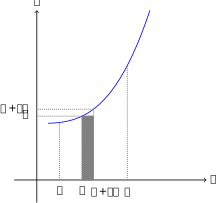
\includegraphics[width=0.5\linewidth]{fy-B-lectnotes_files/figure-latex/22-slice-under-a-curve-1} 

}

\caption{$f(x)$}\label{fig:22-slice-under-a-curve}
\end{figure}

At point \(x\), the curve has a height \(y\) at point \(x + \delta x\) the curve has height \(y + \delta y\) (Figure \ref{fig:22-slice-under-a-curve}).

\begin{notslides}

The area of the shaded rectangle under the curve is \(y\delta x\). As drawn, the area of the rectangle has a value quite close to the area under the curve between \(x\) and \(x + \delta x\). If we chose \(\delta x\) to have a smaller value, then the area of the resulting rectangle would be nearer in size to the area between \(x\) and \(x + \delta x\). The smaller we choose \(\delta x\) to be, the better the approximation to the area. In the limit as \(\delta x \to 0\), the area of the rectangle is exactly the same as the area under the curve.

\end{notslides}

\begin{slidesonly}

\vfill

\begin{itemize}
\tightlist
\item
  shaded area \(y\delta x\)
\item
  ``close'' to area under that part of the curve
\item
  smaller \(\delta x\) \(\implies\) better approximation
\end{itemize}

\vfill
\slide

\end{slidesonly}

Consider now the area \(A\) under the curve between \(a\) and \(b\).

\begin{itemize}
\tightlist
\item
  We split it up into several vertical strips, each of width \(\delta x\).
\item
  Denote the \(x\)-coordinates of the vertical ``chopping lines'' by \(x_0=a, x_1, \dots, x_k=b\).
\item
  An approximation of \(A\) is the sum of the areas of all the rectangles as above, and may be written as
  \[
  A\approx\sum_{i=0}^{k-1}f(x_i)\delta x
  \]
\end{itemize}

\begin{notslides}

where the sign \(\Sigma\) (sigma) means, work out the area of each rectangle in turn then add all the areas together.

\end{notslides}

\begin{itemize}
\tightlist
\item
  As \(\delta x \to 0\), the approximation gets precise. We replace \(\sigma\) by \(\int\)
  (1st Fundamental Theorem of Calculus in reverse):
  \[
  A =\lim\limits_{\delta x\to 0}\sum_{i=0}^{k-1}f(x_i) \delta x = \int_a^b f(x)\,\mathrm{d}x.
  \]
  \slide
\end{itemize}

\begin{example}
Determine the area between the curve \(y=2x^2+3x+1\) and the \(x-\)axis between the values of \(x=1\) and \(x=2\).
\end{example}

\begin{solution}
\leavevmode

(See Figure \ref{fig:23-area-under-2x23x1}.)
\[
A=\int_1^2(2x^2+3x+1)\mathrm{d}x = \left[\frac{2x^3}{3}+\frac{3x^2}{2}+x\right]_1^2 = \left[\frac{16}{3}+\frac{12}{2}+2\right]-\left[\frac{2}{3}+\frac 32 + 1\right] = \frac{61}{6}.
\]

\begin{figure}

{\centering 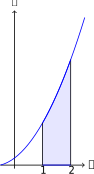
\includegraphics[width=0.2\linewidth]{fy-B-lectnotes_files/figure-latex/23-area-under-2x23x1-1} 

}

\caption{$2x^2+3x+1$}\label{fig:23-area-under-2x23x1}
\end{figure}

\end{solution}

\slide

\subsection{Negative Areas}\label{negative-areas}

If the curve lies below the \(x\)-axis between \(a\) and \(b\), then \(y\) is negative and \(y\delta x\) will also be negative. As a result the integral for regions below the \(x\)-axis will be negative.

This does not mean that the area itself is negative, just that the integral ``counts'' the area below the \(x\)-axis with a minus sign.

Thus some care needs to be taken when using integrals to calculate an ``area under a curve''.

\slide

Consider the curve \(y = x^2 - 3x\) (Figure \ref{fig:24-graph-x23x}). We would like to find the area enclosed between the \(x-\)axis and the values \(x = -1\) and \(x = 5\).

\begin{figure}

{\centering 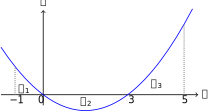
\includegraphics[width=0.5\linewidth]{fy-B-lectnotes_files/figure-latex/24-graph-x23x-1} 

}

\caption{$x^2-3x$}\label{fig:24-graph-x23x}
\end{figure}
\slide

The definite integral over this range is

\begin{notslides}

\[
\int_{-1}^5(x^2-3x)\mathrm{d}x = \left[\frac{x^3}3-\frac{3x^2}2\right]_{-1}^5 = \left[\frac{125}3-\frac{75}2\right]-\left[\frac{-1}3-\frac{3}2\right]=6.
\]

\end{notslides}

\begin{slidesonly}

\[
\int_{-1}^5(x^2-3x)\mathrm{d}x = \phantom{\left[\frac{x^3}3-\frac{3x^2}2\right]_{-1}^5 = \left[\frac{125}3-\frac{75}2\right]}
\]
\vfill

\end{slidesonly}

However, this is not quite the area we may think. This is \(A_1 + A_2 + A_3\) where \(A_2\) is negative, so the value of the definite integral over this range is smaller than the actual area.

\slide

The area of each section is given by

\begin{notslides}

\begin{align*}
A_1&=\int_{-1}^0(x^2-3x)\mathrm{d}x = \left[\frac{x^3}3-\frac{3x^2}2\right]_{-1}^0 = 1.83\\
A_2&=\int_{0}^3(x^2-3x)\mathrm{d}x = \left[\frac{x^3}3-\frac{3x^2}2\right]_{0}^3 = -4.5\\
A_3&=\int_{3}^5(x^2-3x)\mathrm{d}x = \left[\frac{x^3}3-\frac{3x^2}2\right]_{3}^5 = 8.67
\end{align*}
and the total area is given by \(A = A_1 + (-A_2) + A_3 = 1.83 + 4.5 + 8.67 = 15\).

\end{notslides}

\begin{slidesonly}

\begin{align*}
A_1&=\phantom{\int_{-1}^0(x^2-3x)\mathrm{d}x = \left[\frac{x^3}3-\frac{3x^2}2\right]_{-1}^0 = 1.83}\\
A_2&=\phantom{\int_{0}^3(x^2-3x)\mathrm{d}x = \left[\frac{x^3}3-\frac{3x^2}2\right]_{0}^3 = -4.5}\\
A_3&=\phantom{\int_{3}^5(x^2-3x)\mathrm{d}x = \left[\frac{x^3}3-\frac{3x^2}2\right]_{3}^5 = 8.67}
\end{align*}
and the total area is given by \(A = A_1 + (-A_2) + A_3 =\)

\end{slidesonly}

\slide

When we are asked to find the area under a curve for a certain range of \(x\), we must first determine whether the curve crosses the axis in that range. If it does, we need to find the area for each section individually, and then add all the results at the end with the correct signs.

\slide

\begin{example}
Determine the area enclosed between the curve \(y=x^3\) and the \(x-\)axis, between the points \(x=-2\) and \(x=2\).
\end{example}

\begin{solution}
First sketch the curve: Figure \ref{fig:25-graph-x3}.

\begin{figure}

{\centering 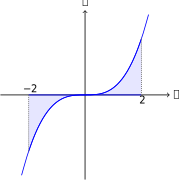
\includegraphics[width=0.4\linewidth]{fy-B-lectnotes_files/figure-latex/25-graph-x3-1} 

}

\caption{$y=x^3$}\label{fig:25-graph-x3}
\end{figure}

We might expect the area to be given by
\[
\int_{-2}^2x^3\mathrm{d}x = \left[\frac{x^4}4\right]_{-2}^2 = \frac{2^4}4-\frac{(-2)^4}4 = 4-4 = 0.
\]
This is clearly not the case. The area to the left of the \(y-\)axis clearly has a negative area while the area to the right has a positive area and these are cancelling one another out.

We actually need
\[
\left|\int_{-2}^0x^3\mathrm{d}x\right|+\left|\int_0^2x^3\mathrm{d}x\right| = \left|\left[\frac{x^4}4\right]_{-2}^0\right|+\left|\left[\frac{x^4}4\right]_{0}^2\right| = \left|0-\frac{(-2)^4}4\right|+\left|\frac{2^4}4-0\right| = 4+4=8.
\]
\end{solution}

\slide

\begin{slidesonly}

\hbox{}
\slide

\end{slidesonly}

\section{Area between two curves}\label{area-between-two-curves}

We may use definite integration to find the area between two curves (or a curve and a straight line).

\begin{example}
Determine the area enclosed between the curve \(y=x^2+1\) and the straight line \(y=7-x\).
\end{example}

\begin{solution}
\leavevmode

In this example we are not told the limits of integration. We must work them out. It is usually best to draw a sketch: Figure \ref{fig:26-graph-x2117x}.

\begin{figure}

{\centering 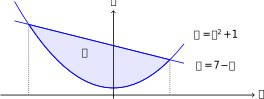
\includegraphics[width=0.5\linewidth]{fy-B-lectnotes_files/figure-latex/26-graph-x2117x-1} 

}

\caption{$y=x^2+1$ and $y=7-x$}\label{fig:26-graph-x2117x}
\end{figure}

We want to find the shaded area. The limits of integration will be the points of intersection of the two curves.

First we need to solve the equations simultaneously to find the \(x-\)co-ordinates of the points of intersection.
\[
7-x=x^2+1\Rightarrow x^2+x-6=0\Rightarrow (x-2)(x+3)=0
\]
Hence we see that the curves intersect at \(x=-3\) and \(x=2\). These are the limits of integration.

From the sketch, the shaded area will be given by

\begin{center}
area under straight line between limits - area under curve between limits.
\end{center}

\begin{align*}
A&=\int_{-3}^2(7-x)\mathrm{d}x - \int_{-3}^2(x^2+1)\mathrm{d}x = \left[7x-\frac{x^2}2\right]_{-3}^2 - \left[\frac{x^3}3+x\right]_{-3}^2\\
&=\left[7\times2-\frac{4}2\right]-\left[7(-3)-\frac92\right]-\left\{\left[\frac{8}3+2\right]-\left[\frac{-27}3-3\right]\right\}\\
&=14-2+21+\frac 92-\frac83-2-\frac{27}3-3=20.83.
\end{align*}
The area is therefore \(20.83\) units\(^2\).

\end{solution}

\slide

\begin{slidesonly}

\hbox{}
\slide

\end{slidesonly}

\begin{example}
Determine the area enclosed between the curve \(y=e^x\) and the curve \(y=e^{-x}\) and \(x=0\) and \(x=2\).
\end{example}

\begin{solution}
\leavevmode

A quick sketch of the curves is on Figure \ref{fig:27-graph-exex}.

\begin{figure}

{\centering 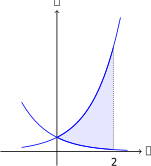
\includegraphics[width=0.4\linewidth]{fy-B-lectnotes_files/figure-latex/27-graph-exex-1} 

}

\caption{$y=e^x$ and $y=e^{-x}$}\label{fig:27-graph-exex}
\end{figure}

\[
A = \int_0^2(e^x-e^{-x})\mathrm{d}x = \left[e^x+e^{-x}\right]_0^2 = (e^2+e^{-2})-(e^0+e^0) = e^2+e^{-2}-2=5.52.
\]

\end{solution}

\slide

\begin{slidesonly}

\hbox{}
\slide

\end{slidesonly}

\section{Parametric Integration}\label{parametric-integration}

If a curve is defined parametrically such that \(x = f(t)\) and \(y = g(t)\) it can be integrated parametrically as follows
\[
\int_a^b y\,\mathrm{d}x = \int_{x=a}^{x=b}g(t)f'(t)\,\mathrm{d}t.
\]
Since \(\mathrm{d}x/\mathrm{d}t = f'(t)\), we may imagine that \(\mathrm{d}x = f'(t)\,\mathrm{d}t\), which happens to be correct. It is normally best to convert the limits of integration into values of \(t\) rather than \(x\). So we find \(a', b'\) such that \(a=f(a'), b = f(b')\) and then the integral becomes
\[
\int_{a'}^{b'}g(t)f'(t)\,\mathrm{d}t.
\]
\slide

\begin{example}
A curve is described by the parametric equations \(x = at^2\) and \(y = 2at\) where \(t\) is a parameter and \(a\) is a constant. Determine the definite integral between \(t = 1\) and \(t = 2\).
\end{example}

\begin{solution}
Here \(x=f(t)=at^2\) and \(y=g(t)=2at\). Hence \(f'(t) = 2at\) and the integral is
\begin{align*}
A &= \int_a^{4a} y\ \mathrm{d}x = \int_{t=1}^{t=2}y\ \mathrm{d}x = \int_1^22at\times 2at\ \mathrm{d}t = \int_1^24a^2t^2\ \mathrm{d}t\\
&= 4a^2\left[\frac{t^3}3\right]_1^2 = 4a^2\left[\frac 83-\frac13\right]=\frac{28}3a^2.
\end{align*}
\end{solution}

\slide

\begin{example}
A curve is described by the parametric equations \(x = \sin(t)\) and \(y = \cos(t)\) where \(t\) is a parameter. Determine the definite integral of \(y\) between \(t = 0\) and \(t = \pi/2\).
\end{example}

\begin{solution}
\begin{align*}
\int_{\sin(0)}^{\sin(\pi/2)}y\ \mathrm{d}x& = \int_0^{\pi/2}\cos(t)\cos(t)\mathrm{d}t = \int_0^{\pi/2}\cos^2(t)\mathrm{d}t = \int_0^{\pi/2}\frac{\cos(2t)+1}{2}\mathrm{d}t\\
& = \frac12\left[\frac{\sin(2t)}2+t\right]_0^{\pi/2} = \frac12\left[0+\pi/2\right]-\frac12\left[0\right]=\frac{\pi}4.
\end{align*}
\end{solution}

\chapter*{Week 7 Exercises}\label{week-7-exercises}
\addcontentsline{toc}{chapter}{Week 7 Exercises}

\section{Sheet 15 - Integration using Partial Fractions}\label{sheet-15---integration-using-partial-fractions}

\begin{enumerate}
\def\labelenumi{\arabic{enumi}.}
\tightlist
\item
  \(\displaystyle\int \frac{2x+3}{x^2+x-30}\ dx\)
\item
  \(\displaystyle\int \frac{17-7x}{(3-x)(2-x)}\ dx\)
\item
  \(\displaystyle\int \frac{5}{x^2-1}\ dx\)
\item
  \(\displaystyle\int \frac{x^2-3x+3}{(x-1)(x-2)(x-3)}\ dx\)
\item
  \(\displaystyle\int \frac{2x^2-2x-2}{x^3-2x^2-x+2}\ dx\)
\item
  \(\displaystyle\int \frac{7}{x^2-4}\ dx\)
\item
  \(\displaystyle\int \frac{5x+2}{x^2-4x+4}\ dx\)
\item
  \(\displaystyle\int \frac{1}{4x^2-9}\ dx\)
\item
  \(\displaystyle\int \frac{1}{x^2-4x-8}\ dx\)
\item
  \(\displaystyle\int \frac{1}{x^2-4x-12}\ dx\)
\item
  \(\displaystyle\int \frac{\cos(x)}{\sin(x)(1+\sin(x))}\ dx\)
\item
  \(\displaystyle\int \frac{\sin(x)}{1-4\cos^2(x)}\ dx\)
\item
  \(\displaystyle\int \frac{e^x}{1-e^{2x}}\ dx\)
\item
  \(\displaystyle\int \frac{1}{x^2-2x-1}\ dx\)
\end{enumerate}

\{Solutions:
1. \(\frac{9}{11}\ln|x+6| + \frac{13}{11}\ln|x-5|+C\);
2. \(-3\ln|x-2|-4\ln|x-3| + C\);
3. \(\frac{5}{2}(\ln|x-1|-\ln|x+1|)+C\);
4. \(\frac{7}{2}\ln|x-1| -13\ln|x-2|+\frac{21}{2}\ln|x-3|+C\);
5. \(\frac{1}{3}\ln|x+1|+\ln|x-1|+\frac{2}{3}\ln|x-2|+C\);
6. \(\frac{7}{4}(\ln|x-2|-\ln|x+2|) +C\);
7. \(5\ln|x-2| - 12/(x-2) +C\);
8. \(\frac{1}{12}(\ln|2x-3|-\ln|2x+3|)+C\);
9. \(\frac{1}{4\sqrt{3}}\left( \ln|x-2\sqrt{3}-2| - \ln|x+2\sqrt{3}-2| \right)+C\);
10. \(\frac{1}{8}(\ln|x-6|-\ln|x+2|) +C\);
11. \(\ln|\sin(x)| - \ln(\sin(x)+1) + C\);
12. \(\frac{1}{4}\left( \ln|2\cos(x)-1| -\ln|2\cos(x)+1| \right) +C\);
13. \(\frac{1}{2}\left( \ln(e^x+1) - \ln|e^x-1| \right) + C\);
14. \(\frac{1}{2\sqrt{2}}\ln\left|\frac{x-1-\sqrt{2}}{x-1+\sqrt{2}}\right| +C\);
\}

\slide

\section{Sheet 16 - Definite Integration}\label{sheet-16---definite-integration}

\subsection*{Exercise 1}\label{exercise-1-6}
\addcontentsline{toc}{subsection}{Exercise 1}

Determine the values of the following definite integrals

\begin{enumerate}
\def\labelenumi{\arabic{enumi}.}
\tightlist
\item
  \(\int_0^2 x^2\ dx\)
\item
  \(\int_0^3 (4-x)^2\ dx\)
\item
  \(\int_0^4 3\sqrt{x}\ dx\)
\item
  \(\int_1^2 t^2+3t\ dt\)
\item
  \(\int_0^{\pi/2}4\cos(\theta) \ d\theta\)
\item
  \(\int_1^2 \cos(\theta)-\sin(\theta)\ d\theta\)
\item
  \(\int_1^9 1/\sqrt{p}\ dp\)
\item
  \(\int_1^2 r^3-1/r\ dr\)
\item
  \(\int_2^3 1/x\ dx\)
\item
  \(\int_1^4 (x+1)/(2\sqrt{x})\ dx\)
\item
  \(\int_2^83/x \ dx\)
\item
  \(\int_{0.5}^1(e^t+e^{-t})/2 \ dt\)
\item
  \(\int_1^4 \sqrt{t}(1+t)^2 \ dt\)
\item
  \(\int_{0.2}^{0.5} \cos(3x)\ dx\)
\item
  \(\int_3^4 (x+1)(2-x)\ dx\)
\item
  \(\int_{\pi/6}^{\pi/4} \sec^2(\theta)\ d\theta\)
\end{enumerate}

\{Solutions:
1. \(8/3\);
2. \(21\);
3. \(16\);
4. \(41/6\);
5. \(4\);
6. \(\sin(2)+\cos(2)-\sin(1)-\cos(1) \approx -0.889\) (\(3\) d.p.);
7. \(4\);
8. \(15/4 - \ln(2) \approx 3.057\) (\(3\) d.p.);
9. \(\ln(3/2) \approx 0.405\) (\(3\) d.p.);
10. \(10/3\);
11. \(3\ln4 \approx 4.159\) (\(3\) d.p.);
12. \(\approx 0.654\) (\(3\) d.p.);
13. \(6904/105 \approx 65.75\) (\(2\) d.p.);
14. \(\frac{1}{3}(\sin(3/2)-\sin(3/5)) \approx 0.1443\) (\(4\) d.p.);
15. \(-41/6 \approx -6.833\) (\(3\) d.p.);
16. \(1-1/\sqrt{3} \approx 0.423\) (\(3\) d.p.);
\}

\slide

\subsection*{Exercise 2}\label{exercise-2-6}
\addcontentsline{toc}{subsection}{Exercise 2}

Evaluate the area bounded by the curve, the x axis and the given ordinates for the following:

\begin{enumerate}
\def\labelenumi{\arabic{enumi}.}
\tightlist
\item
  \(y=x^2-2x\), \(x=0\) and \(x=2\)
\item
  \(y=3x+x^2\), \(x=1\) and \(x=3\)
\item
  \(y=\sin(x)\), \(x=0\) and \(x=\pi/3\)
\item
  \(y=3\cos(3x)\), \(x=\pi/6\) and \(x=\pi/3\)
\item
  \(xy=4\), \(x=3\) and \(x=6\)
\item
  \(y=\sin(x)+\cos(x)\), \(x=\pi/6\) and \(x=1\)
\item
  \(y=1/e^{2x}\), \(x=0\) and \(x=2\)
\item
  \(y=(e^x-e^{-x})/2\), \(x=0\) and \(x=2\)
\item
  \(y=4at\), \(t=0\) and \(t=1\) where \(a\) is a constant
\end{enumerate}

\{Solutions:
1. \(\approx 1.33\) (\(2\) d.p.);
2. \(\approx 20.67\) (\(2\) d.p.);
3. \(0.5\);
4. \(1\);
5. \(\approx 2.77\) (\(2\) d.p.);
6. \(\approx 0.667\) (\(3\) d.p.);
7. \(\approx 0.491\) (\(3\) d.p.);
8. \(\approx 2.76\) (\(2\) d.p.);
9. \(8a^2\);
\}

\chapter{Week 8}\label{week-eight}

Some function can't be, or are difficult to, integrate analytically. However for definite integrals we can use numerical methods to approximate the result. We will learn three methods.

\slide

We defined \(\displaystyle\int_a^bf(x)\,\mathrm{d}x\) using an antiderivative of \(f\); but \(\displaystyle\int_a^bf(x)\,\mathrm{d}x\) also represents the area between the curve and the \(x\)-axis, and we can approximate that to any given degree of accuracy (for reasonable functions \(f\)).

All three methods here start the same way: we chop the area under the curve into a number of vertical strips. Where they differ are the shapes of the regions used to approximate the area(s) of the individual strips.

\begin{itemize}
\tightlist
\item
  Mid-ordinate rule: rectangles (``degree 0 top'')
\item
  Trapezium rule: trapeziums (``degree 1 top'')
\item
  Simpson's rule: ``with a parabola on top'' (``degree 2 top'')
\end{itemize}

\slide

\section{Mid-ordinate Rule}\label{mid-ordinate-rule}

With the \textcolor{red}{\em mid-ordinate rule}\index{mid-ordinate rule}, the curve for which we want to know the area is divided into strips of equal width \(s\), see Figure \ref{fig:28-graph-vertical-strips}.

\begin{figure}

{\centering 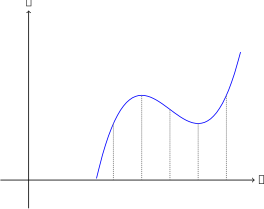
\includegraphics[width=0.6\linewidth]{fy-B-lectnotes_files/figure-latex/28-graph-vertical-strips-1} 

}

\caption{$f(x)$}\label{fig:28-graph-vertical-strips}
\end{figure}
\slide

Considering each strip in turn, we measure the height of the strip, \(h\), along the centre line or mid-ordinate, see Figure \ref{fig:29-mid-ordinate-rule}. The area of the strip is then taken to be the area of a rectangle with height \(h\) and width \(s\).

\begin{figure}

{\centering 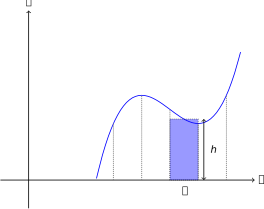
\includegraphics[width=0.6\linewidth]{fy-B-lectnotes_files/figure-latex/29-mid-ordinate-rule-1} 

}

\caption{mid-ordinate rule}\label{fig:29-mid-ordinate-rule}
\end{figure}

\slide

The area of the shaded rectangle \(h \times s\). Depending on the shape of the curve \(f\) in that strip, this area of the rectangle can be smaller or greater than the actual area of the strip under the curve. But if the function \(f\) does not ``wiggle'' too much and the width is small, the approximation is plausible.

\slide

The approximate total area under the curve is the sum of the approximate areas of all the strips so
\[
\text{Total area} = sh_1 + sh_2 + \ldots + sh_n = s(h_1 + h_2 + \ldots + h_n) = s\sum h
\]
where \(\sum h\) is shorthand for the sum of all the values of \(h\).

In words, the total area equals {[}the width of strip{]} times {[}the sum of the mid-ordinates{]}.

\slide

\begin{example}
Use the mid-ordinate rule to approximate the value of the integral
\[
\int_1^4x^2\,\mathrm{d}x
\]
by taking 1, 2 or 3 strips. Compare the values with the correct value.
\end{example}

\begin{solution}
First we know that \(\displaystyle\int_1^4 x^2\,\mathrm{d}x = [x^3/3]_1^4 = 4^3/3-1/3 = 63/3 = 21\).

Using one strip, \(s=3\), the mid-point is \(x=2.5\) and \(h=2.5^2 = 6.25\). Hence the mid-ordinate approximation gives
\[
\int_1^4 x^2 \,\mathrm{d}x \sim 3\times 6.25 = 18.75.
\]
Using two strips, \(s=1.5\), the two mid-points are \(x_1=1.75\) and \(x_2=3.25\) with heights \(h_1=1.75^2=3.0625, h_2=3.25^2=10.5625\). Hence the mid-ordinate approximation gives
\[
\int_1^4 x^2 \,\mathrm{d}x \sim 1.5(3.0625+10.5625)=1.5\times13.625 = 20.4375.
\]
Using three strips, \(s=1\), the three mid-points are \(x_1=1.5, x_2=2.5\) and \(x_3=3.5\) with heights \(h_1=1.5^2=2.25, h_2=2.5^2=6.25, h_3=3.5^2=12.25\). Hence the mid-ordinate approximation gives
\[
\int_1^4 x^2 \,\mathrm{d}x \sim 1\times(2.25+6.25+12.25)=1\times20.75 = 20.75.
\]
\end{solution}

\slide

\begin{slidesonly}

\hbox{}
\slide

\end{slidesonly}

\section{Trapezium rule}\label{trapezium-rule}

For the \textcolor{red}{\em trapezium rule}\index{trapezium rule}, the curve is again divided into strips of equal width \(s\), but this time, the area of each strip is approximated by a trapezium instead of a rectangle, see Figure \ref{fig:30-trapezium-rule}.

\begin{figure}

{\centering 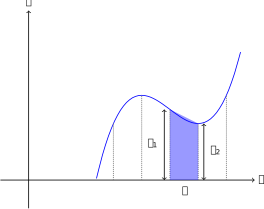
\includegraphics[width=0.7\linewidth]{fy-B-lectnotes_files/figure-latex/30-trapezium-rule-1} 

}

\caption{trapezium rule}\label{fig:30-trapezium-rule}
\end{figure}

For a trapezium, the area is given by
\[
A =\frac12(\text{sum of lengths of parallel sides}) \times(\text{distance between parallel sides})
\]
So for each strip \(\delta A =s(y_1+y_2)/2\). With \(n\) strips, the total area (of the trapeziums) is
\begin{align*}
A& = \frac s2(y_1+y_2) + \frac s2(y_2+y_3) + \ldots + \frac s2(y_{n}+y_{n+1})\\
&= \frac s2\left(y_1+2y_2+2y_3+\ldots 2y_{n}+y_{n+1}\right).
\end{align*}

\slide

\begin{example}
Use the trapezium rule to approximate the integral
\[
\int_1^4x^2\,\mathrm{d}x
\]
by taking 1, 2 or 3 strips.
\end{example}

\begin{solution}
If there is one strip then \(s=3, x_1=1, x_2 = 4, y_1=1^2=1, y_2=4^2=16\). Hence the trapezium rule gives
\[
\int_1^4 x^2 \,\mathrm{d}x \sim \frac32\left(1+16\right) = \frac{51}{2} = 25.5
\]
With two strips then \(s=1.5,x_1=1, x_2=2.5, x_3=4, y_1=1^2=1, y_2=2.5^2=6.25, y_3=4^2=16\). Hence the trapezium rule gives
\[
\int_1^4 x^2 \,\mathrm{d}x \sim \frac{1.5}2\left(1+2\times6.25+16\right) = \frac{354}{16} = 22.125
\]
With three strips then \(s=1,x_1=1, x_2=2, x_3 = 3, x_4=4, y_1=1^2=1, y_2=2^2=4, y_3=3^2=9, y_4=4^2=16\). Hence the trapezium rule gives
\[
\int_1^4 x^2 \,\mathrm{d}x \sim \frac{1}2\left(1+2\times(4+9)+16\right) = \frac{43}{2} = 21.5
\]
\end{solution}

\slide

\begin{slidesonly}

\hbox{}
\slide

\end{slidesonly}

\section{Simpson's Rule}\label{simpsons-rule}

For \textcolor{red}{\em Simpson's rule}\index{Simpson's rule}, we approximate the function in each strip by a quadratic polynomial (i.e.~a piece of a parabola), rather than a line as in the previous two rules --- see Figure \ref{fig:31-simpsons-rule}.

\begin{figure}

{\centering 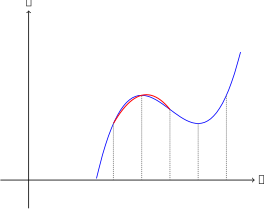
\includegraphics[width=0.7\linewidth]{fy-B-lectnotes_files/figure-latex/31-simpsons-rule-1} 

}

\caption{Simpson's rule}\label{fig:31-simpsons-rule}
\end{figure}

\slide

Given 3 equally spaced points on the curve \((x_1,y_1), (x_2, y_2)\) and \((x_3,y_3)\), we construct a quadratic polynomial \(y=ax^2+bx+c\) which passes through all three points.

In order to simplify the calculations, we can `move' the curve so that the point \(x_2\) coincides with the origin, see Figure \ref{fig:32-simpsons-rule2}. In other words assume that \(x_2=0\). We also let \(x_3-x_2=x_2-x_1=s\) and so \(x_3=s\) and \(x_1=-s\).

\begin{figure}

{\centering 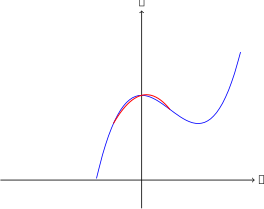
\includegraphics[width=0.7\linewidth]{fy-B-lectnotes_files/figure-latex/32-simpsons-rule2-1} 

}

\caption{Simpson's rule: move to arrange $x_2=0$}\label{fig:32-simpsons-rule2}
\end{figure}

\slide

For the parabola \(y=ax^2+bx+c\) to go through the points \((-s,y_1),(0,y_2),(s,y_3)\) it needs to satisfy
\begin{align*}
y_1&=a(-s)^2+b(-s)+c\\
y_2&=a0^2+b0+c\\
y_3&=as^2+bs+c.
\end{align*}
Solving these gives
\begin{align*}
a&=\frac{y_1+y_3-2y_2}{2s^2}\\
b&=\frac{y_3-y_1}{2s}\\
c&=y_2.
\end{align*}
\slide
The area under that quadratic will then be
\begin{align*}
\int_{-s}^{s}(ax^2+bx+c)\,\mathrm{d}x &= \left[a\frac{x^3}3+b\frac{x^2}2+cx\right]_{-s}^{s}\\
&=\frac{s}{3}\left(y_1+4y_2+y_3\right).
\end{align*}
Notes:

\begin{itemize}
\tightlist
\item
  The formula does not depend on \(x_1,x_2,x_3\) (we've arranged this).
\item
  This approximates \emph{two} strips of width \(s\) rather than one --- so we will want an \emph{even} number of strips.
\end{itemize}

\slide

\begin{notslides}

For approximate integration:

\begin{itemize}
\tightlist
\item
  We split the interval \([a,b]\) over which we are integrating into an even number, say \(2n\), of intervals of length \(s\). Denote the \(x\)-coordinates of the points where we split by \(a=x_1, x_1,\dots,x_{2n+1}=b\).
\item
  We use the above to approximate the area of two consecutive strips: using \(x_1,x_2,x_3\), then \(x_3,x_4,x_5\), etc, until \(x_{2n-1},x_{2n},x_{2n+1}\).
\item
  The sum of the areas gives
  \begin{align*}
  \int_{a}^{b}y\,\mathrm{d}x& \approx \frac s3\left(y_1+4y_2+y_3\right) + \frac s3\left(y_3+4y_4+y_5\right) + \dots + \frac s3\left(y_{2n-1}+4y_{2n}+y_{2n+1}\right)\\
  &=\frac s3\left(y_1+4y_2+2y_3+4y_4+2y_5+\dots +2y_{2n-1}+4y_{2n}+y_{2n+1}\right).
  \end{align*}
\item
  This is known as \textcolor{red}{\em Simpson's rule}\index{Simpson's rule}.
\end{itemize}

\end{notslides}

\begin{slidesonly}

\begin{itemize}
\tightlist
\item
  We split the interval \([a,b]\) over which we are integrating into an even number, say \(2n\), of intervals of length \(s\). Denote the the points where we split by \(a=x_1, x_1,\dots,x_{2n+1}=b\).
\item
  We use the above to approximate the area of two consecutive strips: using \(x_1,x_2,x_3\), then \(x_3,x_4,x_5\), etc, until \(x_{2n-1},x_{2n},x_{2n+1}\). So altogether
  \begin{align*}
  \int_{a}^{b}y\,\mathrm{d}x& \approx \frac s3\left(y_1+4y_2+y_3\right) + \frac s3\left(y_3+4y_4+y_5\right) + \dots\\
  & \qquad\qquad \dots + \frac s3\left(y_{2n-1}+4y_{2n}+y_{2n+1}\right)\\
  &=\frac s3(y_1+4y_2+2y_3+4y_4+2y_5+\dots\\
  & \qquad\qquad \dots +2y_{2n-1}+4y_{2n}+y_{2n+1}).
  \end{align*}
\item
  This is known as \textcolor{red}{\em Simpson's rule}\index{Simpson's rule}.
\end{itemize}

\end{slidesonly}

\slide

\begin{example}
Use Simpson's rule to approximate the integral
\[
\int_1^4x^3\,\mathrm{d}x
\]
by taking 2 and 4 strips.
\end{example}

\begin{solution}
In our above formula we let \(n=1\) and then \(2\).

For \(n=1\) we have \(s=3/2, x_1=1, x_2=2.5, x_3=4\) with \(y_1=1, y_2=15.625, y_3=64\).
\[
\int_1^4x^3\,\mathrm{d}x\sim\frac32\frac13\left[1+4\times15.625+64\right] = 63.75.
\]
For \(n=2\) we have \(s=0.75, x_1=1, x_2=1.75, x_3=2.5, x_4=3.25, x_5=4\) with \(y_1=1, y_2=1.75^3=5.36, y_3 = 2.5^3=15.625, y_4=3.25^3=34.33, y_5=64\).
\[
\int_1^4x^3\,\mathrm{d}x\sim\frac34\frac13\left[1+4\times5.36+2\times15.625+4\times34.33+64\right] = 63.75.
\]

Note that this is actually the exact value:
\[
\int_1^4x^3\,\mathrm{d}x = \left[\frac{x^4}4\right]_1^4 = \frac{4^4}4-\frac14 = \frac{255}4=63.75.
\]
\end{solution}

\slide

\begin{slidesonly}

\hbox{}
\slide
\hbox{}
\slide

\end{slidesonly}

\begin{example}
Use Simpson's rule to approximate the integral
\[
\int_{-1}^1e^{-x^2}\,\mathrm{d}x
\]
by taking 6 strips.
\end{example}

\begin{solution}

This is an example of a function that does not have a suitable antiderivative, so we need to use numerical techniques.

With 6 strips, \(s=1/3\) so we have

\begin{tabular}{l|l}
\hline
$x_1$ & $y_1$\\
\hline
-1 & 0.368\\
\hline
-2/3 & 0.641\\
\hline
-1/3 & 0.895\\
\hline
0 & 1\\
\hline
1/3 & 0.895\\
\hline
2/3 & 0.641\\
\hline
1 & 0.368\\
\hline
\end{tabular}

Hence using Simpson's rule (Figure \ref{fig:33-graph-ex2}):
\[
\int_{-1}^1e^{-x^2}\,\mathrm{d}x \sim \frac19\left[0.368 + 4\times0.641+2\times0.895+4\times1+2\times0.895+4\times0.641+0.368\right] = 1.494.
\]

\begin{figure}

{\centering 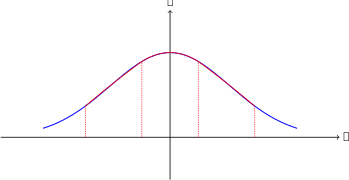
\includegraphics[width=0.7\linewidth]{fy-B-lectnotes_files/figure-latex/33-graph-ex2-1} 

}

\caption{$e^{-x^2}$}\label{fig:33-graph-ex2}
\end{figure}

\end{solution}

\slide

\begin{slidesonly}

\hbox{}
\slide
\hbox{}
\slide

\end{slidesonly}

\begin{example}
Use Simpson's rule to approximate the integral
\[
\int_0^2\frac1{1+x^2}\,\mathrm{d}x
\]
by taking 10 strips and calculate the error involved.
\end{example}

\begin{solution}
With 10 strips, \(s=2/10=0.2\) so we have

\begin{tabular}{l|l}
\hline
$x_1$ & $y_1$\\
\hline
0 & 1\\
\hline
0.2 & 0.96154\\
\hline
0.4 & 0.86207\\
\hline
0.6 & 0.73529\\
\hline
0.8 & 0.60976\\
\hline
1 & 0.5\\
\hline
1.1 & 0.40984\\
\hline
1.4 & 0.33784\\
\hline
1.6 & 0.28090\\
\hline
1.8 & 0.23585\\
\hline
2 & 0.2\\
\hline
\end{tabular}

Hence using Simpson's rule
\begin{align*}
\int_0^2\frac{\mathrm{d}x}{1+x^2} \sim& \frac{0.2}3\left[1 + 0.2\right] +\\
&\frac{0.2}3\times 4\left[0.96154+0.73529+0.5+0.33784+0.23585\right]+\\
&\frac{0.2}3\times 2\left[0.86207+0.60976+0.40984+0.28090\right]\\
&= 1.10715.
\end{align*}
The actual value of the integral is
\[
\int_0^2\frac{\mathrm{d}x}{1+x^2} = \left[\tan^{-1}(x)\right]_0^2 = 1.106587
\]
and so the error is 0.000563.
\end{solution}

\begin{slidesonly}

\hbox{}
\slide
\hbox{}
\slide
\hbox{}
\slide

\end{slidesonly}

\chapter*{Week 8 Exercises}\label{week-8-exercises}
\addcontentsline{toc}{chapter}{Week 8 Exercises}

\section{Sheet 17 Approximate Integration}\label{sheet-17-approximate-integration}

\slide

\subsection*{Exercise 1}\label{exercise-1-7}
\addcontentsline{toc}{subsection}{Exercise 1}

An irregular area has a horizontal base of length 84 mm. The vertical heights measured at regular intervals of 12 mm are, 25.0, 24.5, 23.5, 21.0, 18.0, 14.0, 9.0 mm. Using the midordinate rule, calculate the area of the shape.

\slide

\subsection*{Exercise 2}\label{exercise-2-7}
\addcontentsline{toc}{subsection}{Exercise 2}

An indicator diagram for a steam engine is 90 mm long. Seven evenly spaced ordinates, including the end ordinates are measured with the following results:-
\[
5.10, 4.60, 3.20, 2.70, 2.32, 2.18, 2.06, \text{ mm}
\]
Determine the mean pressure in the engine cylinder using the trapezium rule. The pressure scale is 10 kPa to 1 mm. The mean pressure is given by the ratio of the diagram area to the base length.

\slide

\subsection*{Exercise 3}\label{exercise-3-5}
\addcontentsline{toc}{subsection}{Exercise 3}

By drawing a semi-circle of radius 100 mm, determine the percentage error to two decimal places in the area calculated using i) the mid-ordinate rule ii) the trapezium rule and iii) Simpson's rule. The ordinate spacing is to be taken as 20 mm.

\slide

\subsection*{Exercise 4}\label{exercise-4-4}
\addcontentsline{toc}{subsection}{Exercise 4}

A vehicle starts from rest and its velocity is measured every second for sixty seconds, the results being:-

\begin{tabular}{l|l}
\hline
Velocity (m/s) & Time (s)\\
\hline
0 & 0\\
\hline
1.2 & 1.0\\
\hline
2.4 & 2.0\\
\hline
3.7 & 3.0\\
\hline
5.2 & 4.0\\
\hline
6.0 & 5.0\\
\hline
9.2 & 6.0\\
\hline
\end{tabular}

Determine the distance travelled in the six seconds and the average speed over this time using
Simpson's rule.

\slide

\subsection*{Exercise 5}\label{exercise-5-3}
\addcontentsline{toc}{subsection}{Exercise 5}

Evaluate by Simpson's rule using 10 strips:
\[
\int_0^2\frac{dx}{4+x^2}
\]

\slide

\subsection*{Exercise 6}\label{exercise-6-3}
\addcontentsline{toc}{subsection}{Exercise 6}

The table below relates the values of y at regular intervals of x

\begin{tabular}{l|l}
\hline
$x$ & $y$\\
\hline
1.00 & 2.45\\
\hline
1.25 & 2.80\\
\hline
1.50 & 3.44\\
\hline
1.75 & 4.20\\
\hline
2.00 & 4.33\\
\hline
2.25 & 3.97\\
\hline
2.50 & 3.12\\
\hline
2.75 & 2.38\\
\hline
3.00 & 1.80\\
\hline
\end{tabular}

Using Simpson's rule with 8 intervals evaluate \(\displaystyle\int y\ dx\).

\slide

\subsection*{Exercise 7}\label{exercise-7-1}
\addcontentsline{toc}{subsection}{Exercise 7}

Determine \(\displaystyle\int_0^{\pi/2}\sqrt{\cos(\theta)}\ d\theta\) using 6 intervals.

\slide

\subsection*{Exercise 8}\label{exercise-8}
\addcontentsline{toc}{subsection}{Exercise 8}

A pin moves along a straight guide such that its velocity \(v\) (\(m.s^{-1}\)) when it is at a distance \(s\) (\(m\)) from the start after time \(t\) (\(s\)) is as given below

\begin{tabular}{l|l}
\hline
$v$ (m/s) & $t$ (s)\\
\hline
0 & 0\\
\hline
4.00 & 0.50\\
\hline
7.94 & 1.00\\
\hline
11.68 & 1.50\\
\hline
14.97 & 2.00\\
\hline
17.39 & 2.50\\
\hline
18.25 & 3.00\\
\hline
16.08 & 3.50\\
\hline
0 & 4.00\\
\hline
\end{tabular}

Apply Simpson's rule with 8 intervals to determine the approximate distance travelled by the pin for the time interval \(t = 0\) to \(t = 4\) s

\slide

\subsection*{Exercise 9}\label{exercise-9}
\addcontentsline{toc}{subsection}{Exercise 9}

Evaluate correct to three decimal places

\begin{enumerate}
\def\labelenumi{\roman{enumi}.}
\tightlist
\item
  \(\displaystyle\int_0^1\sqrt{x}\cos(x)\ dx\),
\item
  \(\displaystyle\int_0^1\sqrt{x}\sin(x)\ dx\).
\end{enumerate}

\slide

\subsection*{Exercise 10}\label{exercise-10}
\addcontentsline{toc}{subsection}{Exercise 10}

By using Simpson's rule with six intervals, determine the approximate value of
\[
\int_0^{\pi/2}\sqrt{(2.5-1.5\cos(2\theta))}\ d\theta.
\]

\slide

\subsection*{Exercise 11}\label{exercise-11}
\addcontentsline{toc}{subsection}{Exercise 11}

By using Simpson's rule with 8 intervals, establish the approximate value of
\[
\int_0^1\sqrt{4+x^4}\ dx
\]

{[}Solutions:
1. \(1620\);
2. \(31\,\text{kPa}\);
3. \(0.97\%\), \(3.34\%\), \(1.3\%\);
4. \(3.78\,\text{ms}^{-1}\);
5. \(0.39\);
6. \(6.62\,\text{units}^2\);
7. \(1.19\);
8. \(46.5\,\text{m}\);
9. (i) \(0.529\), (ii) \(0.365\);
10. \(2.41\);
11. \(2.05\);{]}

\chapter{Week 9}\label{week-nine}

In this section, we consider the mean and root mean square values of a function, which is important in studying sinusoidal type functions.

\slide

\section{Mean and RMS Values}\label{mean-and-rms-values}

The \textcolor{red}{\em mean}\index{mean} value for a function \(y = f(x)\) for the range \(a\) to \(b\) is the mean value of all the ordinates in that range. Consider a function \(y = f(x)\) for the values \(x = a\) to \(x = b\), divided into a number of strips of equal width \(\delta x\). Let the mid-ordinate for each strip be \(y_1, y_2, y_3,\ldots,y_n\), see Figure \ref{fig:34-striped-graph}.

\begin{figure}

{\centering 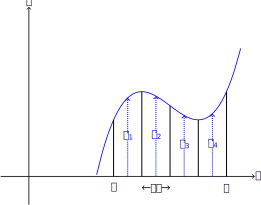
\includegraphics[width=0.7\linewidth]{fy-B-lectnotes_files/figure-latex/34-striped-graph-1} 

}

\caption{$f(x)$}\label{fig:34-striped-graph}
\end{figure}

The mean or average value of the mid-ordinates is
\[
\overline y=\frac{y_1+\ldots+y_n}{n}
\]
\slide

Multiplying the numerator and denominator by \(\delta x\) gives
\[
\overline y=\frac{y_1\delta x+\ldots+y_n\delta x}{n\delta x}
\]
and since \(n\delta x = b - a\) we have
\[
\overline y = \frac{\sum y\delta x}{b-a}.
\]
When the number of strips increases indefinitely such that \(\delta x \to 0\)
\[
\overline y = \frac{1}{b-a}\int_a^b y\ dx.
\]
That is, the mean value of a function between two limits is the area under the curve between those limits divided by the range of \(x\) between those limits.

\slide

\begin{example}
If the velocity \(v\) in \(m/s\) of a body is given by \(v=4t+3\) where \(t\) is in seconds, determine the mean velocity of the body from \(t=2\ \)s to \(t=6\ \)s.
\end{example}

\begin{solution}
\begin{align*}
\text{Mean velocity}& = \frac{1}{6-2}\int_2^6(4t+3)\ dt = \frac 14\left[2t^2+3t\right]_2^6\\
&= \frac 14\left[(2\times36+3\times6) -(2\times4+3\times2)\right] = \frac{76}{4}=19\ m/s.
\end{align*}
\end{solution}

\slide

\subsection{RMS Value}\label{rms-value}

The \textcolor{red}{\em RMS}\index{RMS} (or \textcolor{red}{\em root mean square}\index{root mean square}) value is obtained by taking \(f(x)\), squaring it, finding the mean value and then taking the square root.

Its importance in engineering is demonstrated when a sinusoidal function is investigated, for example when the average value of the current or voltage in a circuit is to be found. For all sine or cosine functions, the mean value over a complete cycle is zero because the curve is equally distributed above and below the \(x-\)axis. However, if the ordinates are squared first, there are then no negative ordinates and an average may be found. Ammeters and voltmeters for a.c. circuits are usually calibrated to find the RMS value.

The RMS value is obtained from
\[
\text{RMS} = \sqrt{\frac{1}{b-a}\int_a^b y^2\ dx}\ .
\]
\slide

\begin{example}
Determine the RMS value of the current in an a.c. circuit given by \(i=20+100\sin(100\pi t)\) between \(t=0\) and \(t=0.02\)s.
\end{example}

\begin{solution}
\begin{align*}
\text{RMS}&= \sqrt{\frac{1}{b-a}\int_a^b i^2\ dt}\\
i&=20+100\sin(100\pi t)\\
i^2&=400+4000\sin(100\pi t)+10000\sin^2(100\pi t)\\
&=400+40000\sin(100\pi t)+10000\times\frac 12(1-\cos(200\pi t))\\
\text{RMS}^2&=\frac1{0.02-0}\int_0^{0.02}(400+40000\sin(100\pi t)+10000\times\frac 12(1-\cos(200\pi t)))\ dt\\
&=\frac1{0.02}\left[400t-\frac{40000\cos(100\pi t)}{100\pi}+5000t-\frac{5000\sin(200\pi t)}{200\pi}\right]_0^{0.02}\\
&=\frac1{0.02}\left[(8-12.732+100-0)-(0-12.732+0-0)\right] = \frac1{0.02}\times108\\
\text{RMS}&=\sqrt{\frac{108}{0.02}}=73.5\text{ A}
\end{align*}
\end{solution}

\chapter*{Week 9 Exercises}\label{week-9-exercises}
\addcontentsline{toc}{chapter}{Week 9 Exercises}

\section{Sheet 17 More problems on Numerical Integration}\label{sheet-17-more-problems-on-numerical-integration}

\slide

\subsection*{Exercise 1}\label{exercise-1-8}
\addcontentsline{toc}{subsection}{Exercise 1}

Use the Simpson's rule with six strips to find an approximate value for
\[
\int_0^{\pi/4}x^2\sin(2x)\ dx,
\]
giving your answer correct to four decimal places.

\slide

\subsection*{Exercise 2}\label{exercise-2-8}
\addcontentsline{toc}{subsection}{Exercise 2}

By using the Simpson's rule with 8 equal intervals, determine
\[
\int_0^4\frac{x+3}{x^2+3x+2}\ dx,
\]
stating the answer to four decimal places.

\slide

\subsection*{Exercise 3}\label{exercise-3-6}
\addcontentsline{toc}{subsection}{Exercise 3}

Using the Simpson's rule with 6 strips, find an approximate value for
\[
\int_4^6\frac{12}{(x-3)(x+1)}\ dx,
\]
giving your answer correct to four decimal places.

{[}Solutions:
1. \(0.1426\);
2. \(2.1230\);
3. \(2.2874\);{]}

\slide

\section{Sheet 18 Mean and RMS Values}\label{sheet-18-mean-and-rms-values}

\slide

\subsection*{Exercise 1}\label{exercise-1-9}
\addcontentsline{toc}{subsection}{Exercise 1}

Determine the mean and RMS values for the following functions

\begin{enumerate}
\def\labelenumi{\roman{enumi}.}
\tightlist
\item
  \(x^2-x\) from \(x=1\) to \(x=3\);
\item
  \(x(3-x)\) from \(x=0\) to \(x=3\);
\item
  \(3\sin(2t)\) from \(t=0\) to \(t=\pi/2\);
\item
  \(2+3\sin(\theta)\) from \(\theta=0\) to \(\theta=\pi\);
\item
  \(\sin(x)\) from \(x=0\) to \(x=\pi\) and from \(x=0\) to \(x=2\pi\);
\item
  \(\cos^2(x)\) from \(x=0\) to \(x=2\pi\);
\item
  \(\sin^2(x)\) from \(x=0\) to \(x=\pi/6\).
\end{enumerate}

\slide

\subsection*{Exercise 2}\label{exercise-2-9}
\addcontentsline{toc}{subsection}{Exercise 2}

Determine the average value of \(y = \sin(3x) + \cos(x)\) for values of \(x\) ranging from \(0\) to \(\pi/6\).

\slide

\subsection*{Exercise 3}\label{exercise-3-7}
\addcontentsline{toc}{subsection}{Exercise 3}

Evaluate the mean values for

\begin{enumerate}
\def\labelenumi{\roman{enumi}.}
\tightlist
\item
  \(1/\sqrt{16-2x^2}\) from \(x=0\) to \(x2\);
\item
  \(1/(1+x^2)\) from \(x=0\) to \(x=1\).
\end{enumerate}

\slide

\subsection*{Exercise 4}\label{exercise-4-5}
\addcontentsline{toc}{subsection}{Exercise 4}

Determine the RMS values for the following functions

\begin{enumerate}
\def\labelenumi{\roman{enumi}.}
\tightlist
\item
  \(x(2-x)\) from \(x=0\) to \(x=2\);
\item
  \(1=\sin(x)\) from \(x=0\) to \(x=2\pi\);
\item
  \(3+2\cos(x)\) from \(x=0\) to \(x=2\pi\);
\item
  \(100\sin(pt)+60\sin(3pt)\) from \(t=0\) to \(t=\pi/p\).
\end{enumerate}

\slide

\subsection*{Exercise 5}\label{exercise-5-4}
\addcontentsline{toc}{subsection}{Exercise 5}

The instantaneous voltage in an AC (alternating current) circuit is given by \(v = 6 + 8\cos(\omega t)\).
Determine the RMS value for the time period \(t = 0\) to \(t = 2\pi/\omega\).

\slide

\subsection*{Exercise 6}\label{exercise-6-4}
\addcontentsline{toc}{subsection}{Exercise 6}

An alternating current is given by \(i = a\sin(\theta)\). Determine the RMS value of the current over a half wave and show that the ratio of the RMS value to the mean value is approximately \(1.11\).

{[}Solutions:
1. (i) \(\overline{y}=2.33\), \(\overline{y}_{\text{RMS}}=2.92\), (ii) \(\overline{y}=1.5\), \(\overline{y}_{\text{RMS}}=1.64\), (iii) \(\overline{y}=1.9\), \(\overline{y}_{\text{RMS}}=2.12\), (iv) \(\overline{y}=3.9\), \(\overline{y}_{\text{RMS}}=4.02\), (v) \(\overline{y}=0.64\), \(\overline{y}_{\text{RMS}}=0.707\), (vi) \(\overline{y}=0.51\), \(\overline{y}_{\text{RMS}}=0.61\), (vii) \(\overline{y}=0.087\), \(\overline{y}_{\text{RMS}}=0.1\);
2. \(\overline{y}=1.59\);
3. (i) \(\overline{y}=0.277\), (ii) \(\overline{y}=0.78\);
4. (i) \(\overline{y}_{\text{RMS}}=0.73\); (ii) \(\overline{y}_{\text{RMS}}=1.22\); (iii) \(\overline{y}_{\text{RMS}}=\sqrt{11}\); (iv) \(\overline{y}_{\text{RMS}}=82.5\);
5. \(\overline{v}_{\text{RMS}}=8.2\);
6. \(\overline{i}=2a/\pi\), \(\overline{i}_{\text{RMS}}=a/\sqrt{2}\), ratio \(=1.11\);{]}

\chapter{Week 10}\label{week-ten}

We look at the important topics of centroids and centers of gravity, before a brief look at volumes and surfaces of revolution.

\slide

\section{Centre of Gravity and Centroids}\label{centre-of-gravity-and-centroids}

Many structures and mechanical systems act as if their masses were concentrated at a single point called the \textcolor{red}{\em center of mass}\index{center of mass} or \textcolor{red}{\em centre of gravity}\index{centre of gravity}. We wish to find out how to locate this point. First let us consider the situation in 1-dimension and then move to consider it in 2-dimensions.

\slide

\subsection{Masses along a line}\label{masses-along-a-line}

\begin{figure}

{\centering 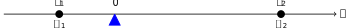
\includegraphics[width=0.7\linewidth]{fy-B-lectnotes_files/figure-latex/35-mass-along-a-line-1} 

}

\caption{mass along a line}\label{fig:35-mass-along-a-line}
\end{figure}

Suppose that the \(x-\)axis is supported by a fulcrum at the origin and we have 2 masses, \(m_1\) and \(m_2\), situated at positions \(x_1\) and \(x_2\) from the origin, see Figure \ref{fig:35-mass-along-a-line}. This is similar to a `see-saw'. Does the system balance, or not? The answer, from experience, depends on both the values of the masses and the positions of the objects. The quantity \(m_1x_1\) is referred to as the \textcolor{red}{\em moment}\index{moment} of the mass \(m_1\) about the origin. Notice that in our figure, \(m_1x_1<0\) and \(m_2x_2>0\). The \textcolor{red}{\em principle of moments}\index{principle of moments} says that the system will balance providing
\[
m_1x_1 + m_2x_2 = 0.
\]

\slide

If we are given a system with more than 2 masses (see Figure \ref{fig:36-mass-along-a-line-many})

\begin{figure}

{\centering 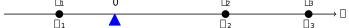
\includegraphics[width=0.7\linewidth]{fy-B-lectnotes_files/figure-latex/36-mass-along-a-line-many-1} 

}

\caption{mass along a line -- many bodies}\label{fig:36-mass-along-a-line-many}
\end{figure}

the principle says that the system will balance providing
\[
\sum m_ix_i = 0.
\]
In principle, we should use the force acting on the body, which is \(m_ig\) where \(g\) is the gravitational acceleration. However the constant \(g\) will cancel out.
\slide
Suppose however, the system does not balance. Can we find a point \(\overline x\) such that if we were to move the fulcrum to that position, the system would balance (see Figure \ref{fig:37-centre-of-mass})?

\begin{figure}

{\centering 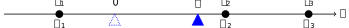
\includegraphics[width=0.7\linewidth]{fy-B-lectnotes_files/figure-latex/37-centre-of-mass-1} 

}

\caption{centre of mass}\label{fig:37-centre-of-mass}
\end{figure}

This would require that
\begin{align*}
\sum(x_i-\overline x)m_i& = 0\\
\sum x_i m_i-\sum{\overline x}m_i& = 0\\
\sum m_ix_i&=\overline x\sum m_i\\
\overline x&=\frac{\sum m_ix_i}{\sum m_i}=\frac{\text{system moment about $O$}}{\text{system mass}}.
\end{align*}

The point \(\overline x\) is called the \textcolor{red}{\em center of mass}\index{center of mass} or \textcolor{red}{\em center of gravity}\index{center of gravity}.
\slide

In order to generalise this situation to 2-dimensions and to consider an `infinite number of points', we need to use integration, rather than a finite sum.

Consider the 2-dimensional strip on Figure \ref{fig:38-2d-rod}, and suppose that the \textcolor{red}{\em density}\index{density} at the point \(x\) is given by \(\rho(x)\).

\begin{figure}

{\centering 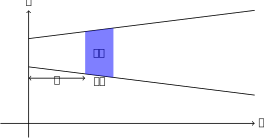
\includegraphics[width=0.6\linewidth]{fy-B-lectnotes_files/figure-latex/38-2d-rod-1} 

}

\caption{2-dimensional rod}\label{fig:38-2d-rod}
\end{figure}
\slide

The density is defined as being
\[
\text{density} = \frac{\text{mass}}{\text{volume}}.
\]
In our case, as we are working in 2-dimensions, the volume becomes the `surface area'. The mass of the shaded region, of area \(\delta A\) (where the width \(\delta x\) is small), is then
\[
\rho(x)\delta A
\]
Summing over all these `small areas' gives
\[
\text{mass} = \int\rho(x)\ dA.
\]
\slide

\begin{example}
Suppose that the rod above is 5 m long with mass per unit length at the point \(x\) given by \(2+x^2/2\ Kg/m\). Find the total mass of the rod.
\end{example}

\begin{solution}
\leavevmode

Take a small rectangular strip of width \(\delta x\) at the point \(x\) so that the mass of this rectangle is
\[
\left(2+\frac{x^2}2\right)\delta x.
\]

\begin{figure}

{\centering 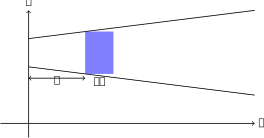
\includegraphics[width=0.6\linewidth]{fy-B-lectnotes_files/figure-latex/39-2d-rod2-1} 

}

\caption{2-dimensional rod}\label{fig:39-2d-rod2}
\end{figure}

Now sum over all such rectangles and allow \(\delta x \to 0\) (in other words compute the integral) to get the mass
\[
\text{mass} = \int_0^5\left(2+\frac{x^2}{2}\right)\ dx = \left[2x+\frac{x^3}{6}\right]_0^5 = 30.8\text{ Kg}.
\]

\end{solution}

\slide

Suppose we wish to find the centre of mass of the rod on Figure \ref{fig:39-2d-rod2}. We use the same principle as in the discrete case when considering a finite number of points except we use an integral rather then a sum. The moment of the small rectangle of width \(\delta x\) is \(x(2+x^2/2)\delta x\). So
\[
\overline x = \frac{\text{moment}}{\text{mass}} = \frac{1}{30.8}\int_0^5 x(2+\frac{x^2}{2})\ dx = \frac{1}{30.8}\left[x^2+\frac{x^4}{8}\right]_0^5 = 3.35.
\]
\slide

\subsection{Centroid of a uniform lamina}\label{centroid-of-a-uniform-lamina}

A \textcolor{red}{\em lamina}\index{lamina} is a solid body in the form of a thin sheet of uniform thickness, with uniform density. As a result, the weight is proportional to the area and the formula for the centre of gravity can have the \(m\) values replaced by \(a\) values where \(a\) represents the area of an element and \(A\) is the total area of the lamina. So
\[
\overline x = \frac{\displaystyle\int xa\ dx}{A},\;\;\; \overline y = \frac{\displaystyle\int ya\ dy}{A}
\]
Then \(\overline x\) and \(\overline y\) are the coordinates of the \textcolor{red}{\em centroid of the area}\index{centroid of the area} or the \textcolor{red}{\em centroid}\index{centroid}.

\slide

Suppose that the centroid of the area bounded by the curve \(y=f(x)\), the \(x-\)axis and the lines \(x=a\) and \(x=b\) is required.

\begin{figure}

{\centering 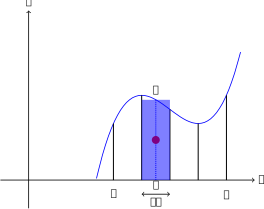
\includegraphics[width=0.5\linewidth]{fy-B-lectnotes_files/figure-latex/40-lamina-1} 

}

\caption{lamina}\label{fig:40-lamina}
\end{figure}

Consider a narrow strip of width \(\delta x\) (see Figure \ref{fig:40-lamina}). The strip can be considered as approximately a rectangle with height \(y\) and area \(y\delta x\). The centre of the area is at the midpoint with coordinate \((x,y/2)\). By summing the moments of the centre of area for each strip we can find the centroid.

\slide

Taking moments about the \(y-\)axis
\[
\overline x = \frac{\displaystyle\int_a^bxy\ dx}{\displaystyle\int_a^b y\ dx}.
\]
Similarly taking moments about the \(x-\)axis
\[
\overline y = \frac{\displaystyle\int_a^b \frac{y^2}2\ dx}{\displaystyle\int_a^b y\ dx}.
\]
\slide

\begin{example}
Determine the centroid of area under the curve \(y=x^2\) between the coordinates \(x=1\) and \(x=3\).
\end{example}

\begin{solution}
\[
\overline x = \frac{\displaystyle\int_1^3xy\ dx}{\displaystyle\int_1^3 y\ dx} = \frac{\displaystyle\int_1^3x^3\ dx}{\displaystyle\int_1^3x^2\ dx} = \frac{\left[\frac{x^4}{4}\right]_1^3}{\left[\frac{x^3}{3}\right]_1^3} = \frac{20}{8.67} = 2.31
\]
\[
\overline y = \frac{\displaystyle\int_1^3\frac{y^2}2\ dx}{\displaystyle\int_1^3 y\ dx} = \frac{\displaystyle\int_1^3\frac{x^4}2\ dx}{\displaystyle\int_1^3x^2\ dx} = \frac{\left[\frac{x^5}{10}\right]_1^3}{8.67} = \frac{24.1}{8.67} = 2.78
\]
The centroid therefore has coordinates \((2.31,2.78)\).
\end{solution}

\slide

\section{Volume and Surface of Revolution}\label{volume-and-surface-of-revolution}

Consider a curve \(y = f(x)\) between the ordinates \(x = a\) and \(x = b\). The volume of revolution is the volume of the equivalent solid body obtained by rotating the curve around the \(x\) or \(y\) axes.

\slide

\subsection{\texorpdfstring{Rotation about the \(x-\)axis}{Rotation about the x-axis}}\label{rotation-about-the-x-axis}

\begin{figure}

{\centering 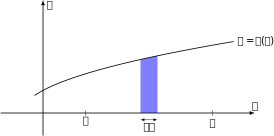
\includegraphics[width=0.5\linewidth]{fy-B-lectnotes_files/figure-latex/41-volume-of-revolution-1} 

}

\caption{volume of revolution}\label{fig:41-volume-of-revolution}
\end{figure}

If the shaded strip in Figure \ref{fig:41-volume-of-revolution} is rotated about the \(x-\)axis then, provided \(\delta x\) is small, it will trace out a disc with thickness \(\delta x\) and volume \(\delta V = \pi y^2\delta x\), where \(y\) is the radius of the disc, see Figure \ref{fig:42-volume-of-revolution2}.
\slide

\begin{figure}

{\centering 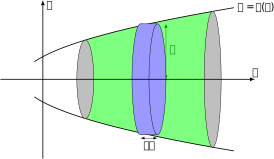
\includegraphics[width=0.5\linewidth]{fy-B-lectnotes_files/figure-latex/42-volume-of-revolution2-1} 

}

\caption{volume of revolution}\label{fig:42-volume-of-revolution2}
\end{figure}

We may sum the volumes generated by all the strips between \(x = a\) and \(x = b\) to obtained the volume of the solid of revolution for the section of curve about the x axis.
Thus the total volume \(V\) is given by
\[
V = \int_a^b\pi y^2\ dx
\]
\slide

\subsection{\texorpdfstring{Rotation about the \(y-\)axis}{Rotation about the y-axis}}\label{rotation-about-the-y-axis}

By a similar method it can be shown that for a rotation about the \(y-\)axis, the volume the solid of revolution will be
\[
V = 2\pi\int_a^bxy\ dx.
\]
\slide

\subsection{Surface area of revolution}\label{surface-area-of-revolution}

The surface area of revolution is the surface area of the body generated by rotating a curve about the \(x\) or \(y\) axes. For a strip as shown in the figure above, the length of arc is approximately \(\delta x\). If the strip is rotated about the \(x\) axis, the surface area generated will be approximately \(\delta S = 2\pi y\delta x\). The surface area of the whole solid generated by rotating the curve around the \(x\) axis between \(x = a\) and \(x = b\) is obtained by summing the contributions to the surface area from each of the elementary strips and we can eventually deduce that
\[
S = 2\pi\int_a^b y\sqrt{1+\left(\frac{dy}{dx}\right)^2}\ dx.
\]
\slide

\begin{example}
\leavevmode

The straight line \(y=mx\) between \(x=0\) and \(x=h\) is rotated about the \(x-\)axis thus generating a right circular cone. Calculate its volume in terms of \(h\) and \(R\) where \(R\) is the \(y\) value at \(x=h\). Find also the surface area of the resultant cone.

\begin{figure}

{\centering 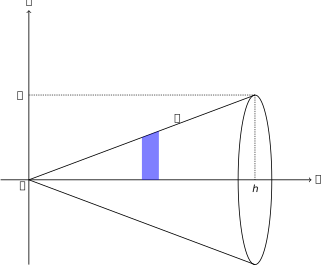
\includegraphics[width=0.6\linewidth]{fy-B-lectnotes_files/figure-latex/43-right-circ-cone-1} 

}

\caption{right-circular-cone}\label{fig:43-right-circ-cone}
\end{figure}

\end{example}

\begin{solution}
See Figure \ref{fig:43-right-circ-cone}.

The volume of the solid of revolution for \(y = mx\) is given by
\[
V = \pi\int_0^hy^2\ dx = \pi\int_0^h (mx)^2\ dx = m^2\pi\int_0^hx^2\ dx = m^2\pi\left[\frac{x^3}3\right]_0^h = m^2\pi\frac{h^3}3.
\]
Now \(m = R/h\) and so
\[
V = \frac13\frac{R^2}{h^2}h^3 = \frac13\pi R^2h.
\]
The surface area is given by
\begin{align*}
S&= 2\pi\int_0^hy\sqrt{1+\left(\frac{dy}{dx}\right)^2}\ dx = 2\pi\int_0^h mx\sqrt{1+m^2}\ dx\\
&= 2m\sqrt{1+m^2}\pi\left[\frac{x^2}2\right]_0^h = m\sqrt{1+m^2}\pi h^2 = \pi R h\sqrt{1+m^2}\\
&= \pi Rl.
\end{align*}
where \(l\) is the length of the inclined line.
\end{solution}

\slide

\begin{example}
A curve is given parametrically as \(x=4t^2, y = 6t-t^2\). Determine the volume generated when the figure bounded by the curve, the \(x-\)axis and the ordinates corresponding to \(t=0\) and \(t=2\) is rotated about the \(x-\)axis.
\end{example}

\begin{solution}
\[
V = \pi\int_a^b y^2\ dx.
\]
Since \(x=4t^2\) then \(dx/dt = 8t\) and so we can write \(dx = 8t\ dt\). Hence
\begin{align*}
V& = \pi\int_0^t(6t-t^2)^28t\ dt = 8\pi\int_0^2(36t^3-12t^4+t^5)\ dt\\
& = 8\pi\left[9t^4-\frac{12t^5}5+\frac{t^6}6\right]_0^2\\
&= 8\pi\times77.87 = 1957 \text{ units}^3.
\end{align*}
\end{solution}

\chapter*{Week 10 Exercises}\label{week-10-exercises}
\addcontentsline{toc}{chapter}{Week 10 Exercises}

\section{Sheet 19 Centroids of area}\label{sheet-19-centroids-of-area}

\slide

\subsection*{Exercise 1}\label{exercise-1-10}
\addcontentsline{toc}{subsection}{Exercise 1}

Determine the positionns of the centroids of the uniform laminae represented by the following curves and indicated boundaries.

\begin{enumerate}
\def\labelenumi{\roman{enumi}.}
\tightlist
\item
  \(y=x^2\), the \(x\)-axis and \(x=0, x=2\);
\item
  \(y=2x^3\), the \(x\)-axis and \(x=1, x=2\);
\item
  The portion of \(y=2x-x^2\) above the \(x\)-axis.
\end{enumerate}

\slide

\subsection*{Exercise 2}\label{exercise-2-10}
\addcontentsline{toc}{subsection}{Exercise 2}

Determine the position of the centroid of the figure bounded by \(y = e^{2x}\), the \(x-\)axis, the \(y-\)axis and the ordinate at \(x = 2\).

\slide

\subsection*{Exercise 3}\label{exercise-3-8}
\addcontentsline{toc}{subsection}{Exercise 3}

Determine the position of the centroid of the figure bounded by the curve \(y = 5\sin(2x)\), the \(x-\)axis and the ordinates at \(x = 0\) and \(x = \pi/6\).

\slide

\subsection*{Exercise 4}\label{exercise-4-6}
\addcontentsline{toc}{subsection}{Exercise 4}

A curve is given parametrically as \(x = at^2, y = 2at\) where \(t\) is a parameter and \(a\) is a constant. Determine the position of the centroid about the for figure bounded by the values \(t = 1\) and \(t = 2\).

{[}Solutions:
1.
(i) \(\overline{x}=1.5\), \(\overline{y}=1.2\),
(ii) \(\overline{x}=1.65\), \(\overline{y}=4.8\),
(iii) \(\overline{x}=1\), \(\overline{y}=0.4\);
2. \(\overline{x}=1.5\), \(\overline{y}=13.6\);
3. \(\overline{x}=0.3\), \(\overline{y}=1.5\);
4. \(\overline{x}=2.66\), \(\overline{y}=1.61\);{]}

\slide

\section{Sheet 20 Volumes of Revolution}\label{sheet-20-volumes-of-revolution}

\slide

\subsection*{Exercise 1}\label{exercise-1-11}
\addcontentsline{toc}{subsection}{Exercise 1}

Determine the volume of the solid of revolution obtained by rotating the curve \(y = x^2\) about

\begin{enumerate}
\def\labelenumi{\roman{enumi}.}
\tightlist
\item
  The \(x-\)axis between the limits \(x = 1\) and \(x = 3\);
\item
  The \(y-\)axis between the same limits.
\end{enumerate}

\slide

\subsection*{Exercise 2}\label{exercise-2-11}
\addcontentsline{toc}{subsection}{Exercise 2}

A cone is generated by rotating the line \(y = x/2\) about the \(x-\)axis from \(x = 0\) to \(x = 10\). Determine the volume of the cone.

\slide

\subsection*{Exercise 3}\label{exercise-3-9}
\addcontentsline{toc}{subsection}{Exercise 3}

Determine the volumes of revolution formed by rotating about the \(x-\)axis the areas between the curves of

\begin{enumerate}
\def\labelenumi{\roman{enumi}.}
\tightlist
\item
  \(y = x^2 - 2x\) and the \(x-\)axis;
\item
  \(y = 3x - x^2\) and the \(x-\) axis.
\end{enumerate}

\slide

\subsection*{Exercise 4}\label{exercise-4-7}
\addcontentsline{toc}{subsection}{Exercise 4}

Determine the volume generated when the plane figure bounded by \(y = 5\cos(2x)\), the \(x-\)axis and the ordinates at values \(x = 0\) and \(x = \pi/4\) rotates about the \(x-\)axis for a complete revolution.

\slide

\subsection*{Exercise 5}\label{exercise-5-5}
\addcontentsline{toc}{subsection}{Exercise 5}

The parametric equations of a curve are given as \(x = 6t^2, y = 2t - t^2\).Determine the volume generated when the plane figure bounded by the curve, the \(x-\)axis and the ordinates corresponding to \(t = 0\) and \(t = 2\) rotates about the \(x-\)axis

{[}Solutions:
1. \(152\);
2. \(126\);
3. (i) \(3.35\), (ii) \(25.4\);
4. \(30.8\);
5. \(40.2\);{]}

\chapter{Week 11}\label{week-eleven}

\slide

\section{Vectors I}\label{vectors-i}

A \textcolor{red}{\em scalar}\index{scalar} quantity has only size or magnitude. Examples of scalars are mass, time, speed \(\ldots\)

A \textcolor{red}{\em vector}\index{vector} quantity has magnitude and direction, examples are force, velocity acceleration, moment, \(\ldots\)

A vector is represented graphically by a straight line with an arrowhead showing its direction. Often the line is drawn to scale so that the magnitude of the vector may be determined by measuring its length.

\begin{center}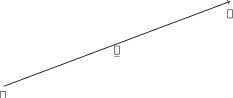
\includegraphics[width=0.4\linewidth]{fy-B-lectnotes_files/figure-latex/44-vectors-1-1} \end{center}

The diagram above shows two ways that vectors are often drawn. To refer to the vector we give it a name. There are many different methods used to indicate that we are referring to a vector quantity. The vector above will often be referred to in books as \(\underline{OP}\) or \(\underline p\) or \(\vec{p}\). The point at which a vector starts is called the initial point. The point at which it ends is called the final point.

Sometimes we are only interested in the magnitude of the vector. In this case we show that we are considering the magnitude only by writing, for example \(|\underline{OP}|\). The vertical lines are called modulus lines and can be used with any of the ways of the different ways of writing a vector. So the vector \(\underline{OP}\) has a length (or magnitude) \(|\underline{OP}|\).

We can multiply a vector by a positive scalar (or ordinary number). This has the effect of leaving the direction the same, but changing the magnitude. For example, below we have the vectors \(\underline a\) and \(3\underline a\). Note that \(3\underline a\) is parallel to \(\underline a\) (has the same direction) but is \(3\) times as long.

\begin{center}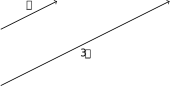
\includegraphics[width=0.4\linewidth]{fy-B-lectnotes_files/figure-latex/45-vectors-2-1} \end{center}

Multiplication by a negative scalar turns the vector around through \(180^\circ\). A position vector indicates the distance and direction that we have to travel from the origin to get to a point. In the diagram below, if \(O\) is the origin then \(\underline{OP}\) is the position vector of the point called \(P\). \(\underline{PQ}\) is called a displacement vector. It shows the distance and direction that we have to travel from \(P\) to get to \(Q\). \(\underline{OQ}\) is the position vector of the point \(Q\). Position vectors always refer to the position of a point relative to the origin. Displacement vectors refer to the position of any point relative to any other.

\begin{center}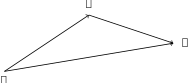
\includegraphics[width=0.4\linewidth]{fy-B-lectnotes_files/figure-latex/46-vectors-3-1} \end{center}

\slide

\subsection{Vector Algebra}\label{vector-algebra}

We have already seen that a vector may be \textcolor{red}{\em multiplied by a scalar}\index{multiplied by a scalar}. If the scalar is positive this changes the magnitude but not the direction of the vector. If the scalar is negative the vector is turned around through \(180^\circ\) and the magnitude is changed.

Two vectors \(a\) and \(b\) are equal if they have the same magnitude and the same direction. They do not actually have to start and finish at the same point.

\begin{center}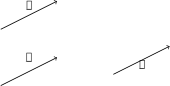
\includegraphics[width=0.4\linewidth]{fy-B-lectnotes_files/figure-latex/47-vectors-4-1} \end{center}

In the above diagram, \(\underline a= \underline b = \underline c\).

If a vector \(\underline b\) has the same magnitude as vector \(\underline a\), but points in the opposite direction then \(\underline b = -\underline a\).

\begin{center}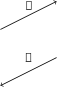
\includegraphics[width=0.15\linewidth]{fy-B-lectnotes_files/figure-latex/48-vectors-5-1} \end{center}

Again it doesn't matter whether they start and finish at the same point or not.

The \textcolor{red}{\em sum}\index{sum} (or \textcolor{red}{\em resultant}\index{resultant}) of two vectors is obtained by placing the initial point of the second vector in the sum at the final point of the first vector in the sum. The sum is then the vector that completes the triangle (i.e.~runs from the initial point of the first to the final point of the second). This is called the triangle law of vector addition.

\begin{center}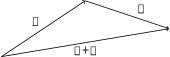
\includegraphics[width=0.4\linewidth]{fy-B-lectnotes_files/figure-latex/49-vectors-6-1} \end{center}

The difference of two vectors is given by \(\underline a + (-\underline b)\), where \(-\underline b\) points in the opposite direction to \(\underline b\). The sum of \(\underline a + (-\underline b)\) is then found from the triangle law above. Hence we write \(\underline a-\underline b = \underline a + (-\underline b)\).

The sum of a set of vectors that form a closed loop is always zero.

\begin{center}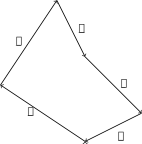
\includegraphics[width=0.4\linewidth]{fy-B-lectnotes_files/figure-latex/50-vectors-7-1} \end{center}

\(\underline a + \underline b + \underline c + \underline d + \underline e = \underline 0\).

\slide

\begin{example}

For the diagram below, state the magnitude of the sum of the vectors \(\underline{AB}\), \(\underline{BC}\), \(\underline{CD}\) and \(\underline{DE}\).

\begin{center}\includegraphics[width=0.4\linewidth]{fy-B-lectnotes_files/figure-latex/51-vectors-8-1} \end{center}

\end{example}

\begin{solution}
The sum of all the vectors starts at the initial point of the first vector and ends at the final point of the last vector. This is the vector \(\underline{AE}\). Its magnitude may be written \(|\underline{AE}|\).
\end{solution}

If a vector joins two points \(A\) and \(B\), then it is equivalent to any other system of vectors that form a path from \(A\) to \(B\). For example the vector \(\underline{AB}\) shown as a solid line below, is equivalent to the sum of the vectors shown dotted.

\begin{center}\includegraphics[width=0.4\linewidth]{fy-B-lectnotes_files/figure-latex/52-vectors-9-1} \end{center}

This fact may be used to solve geometric problems using vectors.

\slide

\begin{example}

For the triangle \(ABC\), if \(D\) is the mid-point of \(AB\) show that
\[
2\underline{AB}+3\underline{BC}+\underline{CA} = 2\underline{DC}.\tag{1}
\]

\begin{center}\includegraphics[width=0.4\linewidth]{fy-B-lectnotes_files/figure-latex/53-vectors-10-1} \end{center}

\end{example}

\begin{solution}
From the triangle
\begin{align*}
\underline{AB}&=2\underline{AD}\tag{2}\\
\underline{BC}&=\underline{BD}+\underline{DC}\tag{3}\\
\underline{CA}&=\underline{CD}+\underline{DA}\tag{4}\\
\end{align*}
Substituting the equations (2), (3) and (4) for the left-hand side of (1) gives
\[
2\underline{AB}+3\underline{BC}+\underline{CA}=4\underline{AD}+3\underline{BD}+3\underline{DC}+\underline{CD}+\underline{DA}.\tag{5}
\]
Now
\begin{align*}
\underline{BD}&=-\underline{AD}\tag{6}\\
\underline{CD}&=-\underline{DC}\tag{7}\\
\underline{DA}&=-\underline{AD}\tag{8}\\
\end{align*}
Substituting these into the right-hand side of equation (5) gives
\[
2\underline{AB}+3\underline{BC}+\underline{CA}=4\underline{AD}-3\underline{AD}+3\underline{DC}-\underline{DC}-\underline{AD}.
\]
So
\[
2\underline{AB}+3\underline{BC}+\underline{CA} = 2\underline{DC}.
\]
\end{solution}

\slide

\section{Vectors II}\label{vectors-ii}

\subsection{Unit Vectors}\label{unit-vectors}

A \textcolor{red}{\em unit vector}\index{unit vector} is a vector with magnitude of 1.

If \(\underline a\) is a vector with magnitude \(|\underline a|\), then a unit vector with the same direction is written \(\hat{\underline a}\) where \(|\hat{\underline a}| = 1\). Notice that
\[
\hat{\underline a} = \frac1{|\underline a|}{\underline a}.
\]
For vector systems, there are three special unit vectors \(\underline i\), \(\underline j\) and \(\underline k\). These vectors for a set of axes for a vector system and are perpendicular to each other (like \(x\), \(y\) and \(z\) in Cartesian notation). Strictly, they should be written \(\hat{\underline i}, \hat{\underline j}\) and \(\hat{\underline k}\) to indicate that they are unit vectors, but they are used so often that the circumflex, \(\hat{}\), tends to get left off. The axis vectors are arranged as a righthand system. This means that a screw turned from \(\underline i\) to \(\underline j\) should travel up the \(\underline k\) axis.

\begin{center}\includegraphics[width=0.85\linewidth]{fy-B-lectnotes_files/figure-latex/54-vectors-11-1} \end{center}

A vector may be resolved in terms of its components in the direction of the unit axis vectors. We shall start by considering a two dimensional vector. For this we need only the \(\underline i\) and \(\underline j\) axes.

\begin{center}\includegraphics[width=0.33\linewidth]{fy-B-lectnotes_files/figure-latex/55-vectors-12-1} \end{center}

The vector \(\underline r\) makes an angle \(\theta\) with the \(\underline i\) axis and has magnitude \(|\underline r| = r\). We may say that to get to the point \(R\), we have to start at the \(\underline i\) axis, turn through an angle \(\theta\) and then travel a distance \(r\) from the origin. Alternatively, we may get to \(R\), by travelling a distance along the \(\underline i\) axis and then a distance up in the direction of the \(\underline j\) axis. The distance to be travelled along the \(\underline i\) axis is \(r\cos(\theta)\) and the distance to be travelled up in the direction of the \(\underline j\) axis is \(r\sin(\theta)\). The vector \(\underline r\) may thus be written as \(\underline r = r\cos(\theta) \underline i + r\sin(\theta)\underline j\).

When written in this form \(\underline r\) is said to be resolved into its \textcolor{red}{\em component vectors}\index{component vectors}.

\slide

A 2D vector may be given in its component form as, for example \(\underline r = 6\underline i + 5\underline j\).

If we have two 2D vectors lying in the same plane, then they are said to be co-planar vectors.

\begin{center}\includegraphics[width=0.33\linewidth]{fy-B-lectnotes_files/figure-latex/56-vectors-13-1} \end{center}

The vectors \(\underline a\) and \(\underline b\) are co-planar.

\slide

We may also write 3D vectors in terms of their unit vectors, but this time we need all three axes.

\begin{center}\includegraphics[width=0.45\linewidth]{fy-B-lectnotes_files/figure-latex/57-vectors-14-1} \end{center}

The vector \(\underline r\) projects a length \(a\) onto the \(\underline i\) axis, a length \(b\) onto the \(\underline j\) axis and a length \(c\) onto the \(\underline k\) axis, so \(\underline r\) may be written \(\underline r = a\underline i + b\underline j + c\underline k\).

\slide

\subsection{Vector algebra with component vectors}\label{vector-algebra-with-component-vectors}

When a vector is written in terms of its components, then the sum of two vectors is the sum of the components for each direction. e.g.
\[
\underline a = 6\underline i + 2\underline j, \underline b = 5\underline i - \underline j\;\text{ so }\;\underline a + \underline b = (6 + 5)\underline i + (2 + (-1))\underline j = 11\underline i + \underline j.
\]
Note that \(1\underline i, 1\underline j\), or \(1\underline k\) are usually written as just \(i\underline , \underline j\) or \(\underline k\).

Similarly
\[
\underline a = 5\underline i + 4\underline j - \underline k, \underline b = 3\underline i - 7\underline j + 8\underline k\;\text{ so }\; \underline a + \underline b = (5+3)\underline i + (4 - 7)\underline j + (-1 + 8)\underline k = 8\underline i -3\underline j + 7\underline k.
\]

When a vector is written in terms of components, the difference of the two vectors is the difference of the components for each direction. e.g.
\[
\underline a = 5\underline i + 4\underline j - \underline k, \underline b = 3\underline i - 7\underline j + 8\underline k\;\text{ so }\; \underline a - \underline b = (5 - 3)\underline i + (4 - (-7))\underline j + ((-1) - 8)\underline k = 2\underline i + 11\underline j -9\underline k.
\]
When a vector written in terms of components is multiplied by a scalar, each component is multiplied by that scalar e.g.
\[
\underline a = 5\underline i + 4\underline j - \underline k\;\text{ so }\;3\underline a = 15\underline i + 12\underline j - 3\underline k.
\]
\slide

\subsection{The magnitude of a vector}\label{the-magnitude-of-a-vector}

\begin{center}\includegraphics[width=0.33\linewidth]{fy-B-lectnotes_files/figure-latex/58-vectors-15-1} \end{center}

The vector \(\underline r = a\underline i + b\underline j\). From Pythagoras' theorem, the magnitude of vector \(|\underline r| = \sqrt{a^2+b^2}\). In three dimensions, if \(\underline r = a\underline i + b\underline j + c\underline k\), then \(|\underline r| = \sqrt{a^2+b^2+c^2}\).

\begin{center}\includegraphics[width=0.45\linewidth]{fy-B-lectnotes_files/figure-latex/59-vectors-16-1} \end{center}

\slide

\subsection{Finding a unit vector}\label{finding-a-unit-vector}

If \(\underline r = a\underline i + b\underline j + c\underline k\), then its magnitude is \(|r| = \sqrt{a^2+b^2+c^2}\). That is the length of the vector is \(\sqrt{a^2+b^2+c^2}\). If we want to find a vector that has the same direction as \(\underline r\), but has length of 1, i.e.~the unit vector \(\underline{\hat r}\), then we must divide \(\underline r\) by its own magnitude. So if \(\underline r = a\underline i + b\underline j + c\underline k\), then
\[
\underline{\hat r} = \frac{1}{\sqrt{a^2+b^2+c^2}}(a\underline i+b\underline j+c\underline k)
\]
which can be written
\[
\underline{\hat r} = \frac{a}{\sqrt{a^2+b^2+c^2}}\underline i+\frac{b}{\sqrt{a^2+b^2+c^2}}\underline j+\frac{c}{\sqrt{a^2+b^2+c^2}}\underline k
\]
or
\[
\underline{\hat r} = \frac{a}{|\underline r|}\underline i+\frac{b}{|\underline r|}\underline j+\frac{c}{|\underline r|}\underline k
\]
\slide

\begin{example}

If \(\underline r = 5\underline i+2\underline j-\underline k\), find a unit vector that is

\begin{enumerate}
\def\labelenumi{\alph{enumi}.}
\tightlist
\item
  parallel to \(\underline r\),
\item
  has the opposite direction to \(\underline r\).
\end{enumerate}

\end{example}

\begin{solution}

\(|\underline r| = \sqrt{5^2+2^2+1^2} = \sqrt{25+4+1} = \sqrt{30}\).

\begin{enumerate}
\def\labelenumi{\alph{enumi}.}
\tightlist
\item
  The unit vector in the direction of \(\underline r\) is
  \[
  \underline{\hat r} = \frac5{\sqrt{30}}\underline i+\frac2{\sqrt{30}}\underline j-\frac1{\sqrt{30}}\underline k.
  \]
\item
  The unit vector in the opposite direction is
  \[
  -\underline{\hat r} = -\left(\frac{5}{\sqrt{30}}\underline i+\frac{2}{\sqrt{30}}\underline j-\frac{1}{\sqrt{30}}\underline k\right) = -\frac{5}{\sqrt{30}}\underline i-\frac{2}{\sqrt{30}}\underline j+\frac{1}{\sqrt{30}}\underline k
  \]
\end{enumerate}

\end{solution}

\slide

\subsection{Direction Cosines}\label{direction-cosines}

The \textcolor{red}{\em direction cosines}\index{direction cosines} of a vector are the cosines of the angles that that vector makes with each of
the three axes. The angles are marked \(\alpha, \beta\) and \(\gamma\) in the figure below

\begin{center}\includegraphics[width=0.55\linewidth]{fy-B-lectnotes_files/figure-latex/60-vectors-17-1} \end{center}

The direction cosines are
\[
l = \cos(\alpha) = \frac{a}{|\underline r|},\;\;m = \cos(\beta) = \frac{b}{|\underline r|},\;\;n = \cos(\gamma) = \frac{c}{|\underline r|}
\]
\slide

\begin{example}
Find the direction cosines of the vector \(\underline r = 3\underline i + 4\underline j - 5\underline k\).
\end{example}

\begin{solution}
The magnitude of \(\underline r\) is \(|\underline r| = \sqrt{3^2+4^2+5^2} = \sqrt{9+16+25} = \sqrt{50}\).

The direction cosines of \(\underline r\) are then
\[
l = \frac{3}{\sqrt{50}},\;\;m = \frac{4}{\sqrt{50}},\;\;n = \frac{-5}{\sqrt{50}}
\]
\end{solution}

\slide

\subsection{The angle between two vectors}\label{the-angle-between-two-vectors}

\begin{center}\includegraphics[width=0.33\linewidth]{fy-B-lectnotes_files/figure-latex/61-vectors-18-1} \end{center}

If we have two vectors \(\underline a\) and \(\underline b\) where \(\underline a\) has direction cosines \(l_a, m_a, n_a\) and \(\underline b\) has direction cosines \(l_b, m_b, n_b\), then the cosine of the angle \(\theta\) between the vectors is given by:
\[
\cos(\theta) = l_al_b + m_am_b + n_an_b.
\]
\slide

\begin{example}
Determine the angle between the two vectors and \(\underline a = 2\underline i + 3\underline j + 4\underline k\) and \(\underline b = 4\underline i - 3\underline j + 2\underline k\).
\end{example}

\begin{solution}
\[
|\underline a| = \sqrt{2^2+3^2+4^2} = \sqrt{29},\;\;|\underline b| = \sqrt{4^2+3^2+2^2} = \sqrt{29}.
\]
So \(\underline a\) has direction cosines
\[
l_a = \frac{2}{\sqrt{29}},\;\;m_a = \frac{3}{\sqrt{29}},\;\;n_a = \frac{4}{\sqrt{29}}
\]
and \(\underline b\) has direction cosines
\[
l_b = \frac{4}{\sqrt{29}},\;\;m_b = \frac{-3}{\sqrt{29}},\;\;n_b = \frac{2}{\sqrt{29}}
\]
The cosine of the angle \(\theta\) between the two vectors is given by
\[
\cos(\theta) = \frac{2}{\sqrt{29}}\frac{4}{\sqrt{29}}+\frac{3}{\sqrt{29}}\frac{-3}{\sqrt{29}}+\frac{4}{\sqrt{29}}\frac{2}{\sqrt{29}} = \frac{8}{29}-\frac{9}{29}+\frac{8}{29} = \frac{7}{29}.
\]
Hence the angle is \(\theta = \cos^{-1}(7/29) = 76^\circ\).
\end{solution}

\slide

\section{Vectors III}\label{vectors-iii}

\subsection{Multiplication of vectors}\label{multiplication-of-vectors}

We know from studying mechanical systems that there are two possible situations when two vectors are multiplied together. A vector multiplied by a vector can result in a scalar quantity, for example, a force (vector) multiplied by the distance (vector) an object moves as a result of that force gives the amount of work (scalar) done by that force. A vector multiplied by a vector can also result in a vector quantity, for example a force (vector) multiplied by the perpendicular distance (vector) of that force from a given point, gives the moment (vector) of that force about the point. Since there may be two different forms multiplying vectors together, we can deduce that there are two different types of vector multiplication; one that results in a scalar quantity and one that results in a vector quantity.

\slide

\subsection{The scalar or dot product}\label{the-scalar-or-dot-product}

The scalar product of two vectors has a scalar quantity as its result.

The scalar product of two vectors \(\underline a\) and \(\underline b\) is defined as
\[
\underline a \cdot\underline b = |\underline a||\underline b|\cos(\theta)
\]
where \(\theta\) is the angle between the two vectors as shown below

\begin{center}\includegraphics[width=0.3\linewidth]{fy-B-lectnotes_files/figure-latex/62-vectors-19-1} \end{center}

If \(\underline a\) and \(\underline b\) are parallel then \(\theta = 0^\circ\) and \(\cos(\theta) = 1\), so \(\underline a \cdot\underline b = |\underline a||\underline b|\).

If \(\underline a\) and \(\underline b\) are perpendicular then \(\theta = 90^\circ\) and \(\cos(\theta) = 0\) so \(\underline a \cdot\underline b = 0\).

\slide

If \(\underline a\) and \(\underline b\) are given in terms of component vectors as \(\underline a = a_1\underline i + a_2\underline j + a_3\underline k\) and \(\underline b = b_1\underline i + b_2\underline j + b_3\underline k\) then
\[
\underline a \cdot\underline b = a_1b_1 + a_2b_2 + a_3b_3.
\]
\slide

\begin{example}
Find the scalar product of \(\underline a = 3\underline i + 2\underline j - 6\underline k\) and \(\underline b = -\underline i + 5\underline j - \underline k\).
\end{example}

\begin{solution}
\[
\underline a\cdot\underline b = a_1b_1 + a_2b_2 + a_3b_3 = (3)(-1)+(2)(5)+(-6)(-1) = -3+10+6=13.
\]
The scalar product of the vectors is 13.
\end{solution}

Now since the scalar product is defined as
\[
\underline a \cdot\underline b = |\underline a||\underline b| \cos(\theta)\tag{1}
\]
it gives us another way of finding the angle \(\theta\) between two vectors. We can re-arrange equation (1) to give
\[
\cos(\theta) = \frac{\underline a\cdot\underline b}{|\underline a||\underline b|}.\tag{2}
\]
\slide

\begin{example}
Using the vectors from the previous example, \(\underline a = 3\underline i + 2\underline j - 6\underline k\) and \(\underline b = -\underline i + 5\underline j - \underline k\), we found that \(\underline a\cdot\underline b = 13\).
Also, \(|\underline a| = \sqrt{3^2+2^2+(-6)^2}=\sqrt{49}=7\) and \(|\underline b| = \sqrt{(-1)^2+5^2+(-1)^2} = \sqrt{27}\) so from equation (2)
\[
\cos(\theta) = \frac{13}{7\sqrt{27}} = 0.3574
\]
and thus \(\theta = \cos^{-1}(0.3574) = 69^\circ\).
\end{example}

\slide

\begin{example}
Find the unit vector perpendicular to the vector \(4\underline i+4\underline j-7\underline k\) and to the vector \(3\underline i - 2\underline j+\underline k\)
\end{example}

\begin{solution}
Let the vector which is perpendicular to the two given vectors be \(p\underline i + q\underline j + r\underline k\).

If the vectors are perpendicular then the scalar product is zero since the angle between them is \(90^\circ\) so
\[
(4\underline i + 4\underline j - 7\underline k) \cdot (p\underline i + q\underline j + r\underline k) = 0\tag{1}
\]
and
\[
(3\underline i - 2\underline j + \underline k) \cdot (p\underline i + q\underline j + r\underline k) = 0.\tag{2}
\]
Evaluating the scalar products (1) and (2) gives
\begin{align*}
4p + 4q -7r& = 0\tag{3}\\
3p - 2q + r& = 0\tag{4}
\end{align*}
We now solve equations (3) and (4) simultaneously
\begin{align*}
4p + 4q - 7r& = 0&(3)\\
6p - 4q + 2r& = 0 &(4 \times 2)\\
\end{align*}
therefore by adding \(10p - 5r = 0\) so
\[
r = 2p.\tag{5}
\]
Substituting into (4) gives \(3p - 2q + 2p = 0\) so
\[
q = \frac52p.\tag{6}
\]
We may choose any value for \(p\) and, provided \(q\) and \(r\) have the relationships (5) and (6) with our chosen value, the vector will be perpendicular to the given vectors. We will choose \(p = 2\), then \(r= 4\) and \(q = 5\) so
\[
p\underline i + q\underline j + r\underline k = 2\underline i + 5\underline j + 4\underline k.
\]
We were asked to find the unit vector. The magnitude of \(2\underline i + 5\underline j + 4\underline k = \sqrt{45} = 3\sqrt{5}\) so the unit vector perpendicular to the given vectors is
\[
\frac{2}{3\sqrt{5}}\underline i+\frac{5}{3\sqrt{5}}\underline j+\frac{4}{3\sqrt{5}}\underline k.
\]
\end{solution}

\slide

\subsection{The vector or cross product}\label{the-vector-or-cross-product}

The vector product of two vectors has as its result a vector.

The vector product is defined as \(\underline a \times\underline b = |\underline a||\underline b|\sin(\theta)\underline{\hat n}\).

That is to say that the magnitude of \(\underline a\times\underline b\) is \(|\underline a||\underline b|\sin(\theta)\) where \(\theta\) is the angle between \(\underline a\) and \(\underline b\) and, since it is a vector, it must also have a direction so \(\underline{\hat n}\) indicates the direction. For a vector product, \(\underline {\hat n}\) is always perpendicular to both \(\underline a\) and \(\underline b\). For \(\underline {\hat n}\) to be perpendicular to \(\underline a\) and \(\underline b\), it could either point in the direction shown below, or in the opposite direction, however for a vector product, \(\underline {\hat n}\) always forms a right-hand set of axes (like \(\underline i, \underline j\) and \(\underline k\)). The vector in the opposite direction (shown dotted) would be obtained from \(\underline b\times\underline a\).

\begin{center}\includegraphics[width=0.45\linewidth]{fy-B-lectnotes_files/figure-latex/63-vectors-20-1} \end{center}

If \(\underline a\) and \(\underline b\) are parallel (i.e.~\(\theta = 0\)), then since \(\sin(\theta) = 0, \underline a \times\underline b = {\underline 0}\).

If \(\underline a\) and \(\underline b\) are perpendicular (i.e.~\(\theta = 90^\circ\)) then since \(\sin(90^\circ)= 1, \underline a \times\underline b = |\underline a||\underline b|\underline {\hat n}\)

If \(\underline a\) and \(\underline b\) are specified in terms of their component vectors, so that \(\underline a = a_1\underline i + a_2\underline j + a_3\underline k\) and \(\underline b = b_1\underline i + b_2\underline j + b_3\underline k\) then
\[
\underline a \times\underline b = \left|\begin{array}{ccc}\underline i&\underline j&\underline k\\a_1&a_2&a_3\\b_1&b_2&b_3\\\end{array}\right|.
\]
\slide

\begin{example}
Find the vector product of \(\underline a=3\underline i+2\underline j-6\underline k\) and \(\underline b=-\underline i + 5\underline j-\underline k\).
\end{example}

\begin{solution}
\begin{align*}
\underline a \times\underline b& = \left|\begin{array}{ccc}\underline i&\underline j&\underline k\\3&2&-6\\-1&5&-1\\\end{array}\right|\\
&= \underline i((2)(-1)-(-6)(5))-\underline j((3)(-1)-(-6)(-1))+\underline k((3)(5)-(2)(-1))\\
&=28\underline i+9\underline j+17\underline k.
\end{align*}
\end{solution}

\slide

\begin{example}
Find a unit vector which is perpendicular to the vector \(4\underline i+4\underline j-7\underline k\) and to the vector \(3\underline i - 2\underline j+\underline k\).
\end{example}

\begin{solution}
From the definition of the vector product, a vector perpendicular to both these vectors is given by
\begin{align*}
(4\underline i+4\underline j-7\underline k) \times(3\underline i - 2\underline j+\underline k)& = \left|\begin{array}{ccc}\underline i&\underline j&\underline k\\4&4&-7\\3&-2&1\\\end{array}\right|\\
&= \underline i((4)(1)-(-7)(-2))\\
&\phantom{= }-\underline j((4)(1)-(-7)(3))\\
&\phantom{= }+\underline k((4)(-2)-(4)(3))\\
&=-10\underline i-25\underline j-20\underline k.
\end{align*}
So a \textbf{\emph{unit vector}} perpendicular to both given vectors is
\[
\frac{-10}{15\sqrt{5}}\underline i-\frac{25}{15\sqrt{5}}\underline j-\frac{20}{15\sqrt{5}}\underline k = \frac{-2}{3\sqrt{5}}\underline i-\frac{5}{3\sqrt{5}}\underline j-\frac{4}{3\sqrt{5}}\underline k.
\]
\end{solution}

\slide

\subsection{The scalar triple product}\label{the-scalar-triple-product}

If we have three vectors \(\underline a, \underline b\) and \(\underline c\) then the scalar triple product of those vectors is defined as \(\underline a \cdot(\underline b\times\underline c)\).

Note that the vector product must be evaluated first, then the scalar product.

The scalar triple product gives the volume of a parallelepiped with edges defined by the vectors \(\underline a, \underline b\) and \(\underline c\).

\begin{center}\includegraphics[width=0.45\linewidth]{fy-B-lectnotes_files/figure-latex/64-vectors-21-1} \end{center}

\slide

\begin{example}
Find the volume of a parallelepiped with edges \(\underline a = 2\underline i - 3\underline j + 4\underline k, \underline b = \underline i + 2\underline j - \underline k\) and \(\underline c = 3\underline i - \underline j + \underline 2\).
\end{example}

\begin{solution}
The volume is given by \(\underline a \cdot(\underline b\times\underline c)\). First we calculate the vector product
\[
\underline b \times\underline c = \left|\begin{array}{ccc}\underline i&\underline j&\underline k\\2&-3&4\\3&-1&2\\\end{array}\right| = 3\underline i-5\underline j-7\underline k.
\]
and now
\[
\underline a \cdot(\underline b\times\underline c) = (2\underline i - 3\underline j + 4\underline k)\cdot(3\underline i-5\underline j-7\underline k) = -7.
\]
The volume is therefore \(7\) units (and the -ve sign tells us that the system was not right handed).
\end{solution}

\slide

\subsection{The vector triple product}\label{the-vector-triple-product}

If we have three vectors \(\underline a, \underline b\) and \(\underline c\) then the vector triple product of those vectors is defined as
\[
\underline a \times (\underline b \times\underline c)
\]

\begin{example}
Find the vector triple product \(\underline a \times (\underline b \times\underline c)\) where \(\underline a = 2\underline i - 3\underline j + 4\underline k, \underline b = \underline i + 2\underline j - \underline k\) and \(\underline c = 3\underline i - \underline j + \underline 2\).
\end{example}

\begin{solution}
From the previous example, \(\underline b \times\underline c = 3\underline i-5\underline j-7\underline k\).
\[
\underline a \times (\underline b \times\underline c) = \left|\begin{array}{ccc}\underline i&\underline j&\underline k\\2&-3&4\\3&-5&7\end{array}\right| = 41\underline i+26\underline j-\underline k
\]
\end{solution}

\chapter*{Week 11 Exercises}\label{week-11-exercises}
\addcontentsline{toc}{chapter}{Week 11 Exercises}

\section{Sheet 21 Vectors I}\label{sheet-21-vectors-i}

\subsection*{Exercise 1}\label{exercise-1-12}
\addcontentsline{toc}{subsection}{Exercise 1}

Two vectors \(\underline A\) and \(\underline B\) are at right angles. Find

\begin{enumerate}
\def\labelenumi{\roman{enumi}.}
\tightlist
\item
  the magnitude of the vector \(\underline A+\underline B\) if \(|\underline A| = 1\) and \(|\underline B| = 2\).
\item
  the magnitude of the vector \(\underline A+\underline B\) if \(|\underline A|=20\) and \(|\underline B| = 21\).
\end{enumerate}

\slide

\subsection*{Exercise 2}\label{exercise-2-12}
\addcontentsline{toc}{subsection}{Exercise 2}

Determine the resultant of the vectors \(\underline A, \underline B, \underline C\) and \(\underline D\) given that \(\underline A = 20\) km \(3o^\circ\) S of E, \(\underline B = 50\) km due W, \(\underline C = 40\) km NE and \(\underline D=30\) km SW.

\slide

\subsection*{Exercise 3}\label{exercise-3-10}
\addcontentsline{toc}{subsection}{Exercise 3}

An object \(P\) is acted on by three forces as shown on Figure \ref{fig:65-res-force}. All forces lie in the same plane (are \emph{co-planar}). Determine the required force and its direction so as to prevent \(P\) from moving.

\begin{figure}

{\centering \includegraphics[width=0.5\linewidth]{fy-B-lectnotes_files/figure-latex/65-res-force-1} 

}

\caption{resultant force}\label{fig:65-res-force}
\end{figure}
\slide

\subsection*{Exercise 4}\label{exercise-4-8}
\addcontentsline{toc}{subsection}{Exercise 4}

For the triangle on Figure \ref{fig:66-triangles}, prove by vectors that the line \(DE\), where \(D\) and \(E\) are the mid-points of \(AB\) and \(AC\) respectively, is half the length of the side \(BC\).

\begin{figure}

{\centering \includegraphics[width=0.5\linewidth]{fy-B-lectnotes_files/figure-latex/66-triangles-1} 

}

\caption{triangles}\label{fig:66-triangles}
\end{figure}

\slide

\subsection*{Exercise 5}\label{exercise-5-6}
\addcontentsline{toc}{subsection}{Exercise 5}

The quadrilateral \(ABCD\) shown on Figure \ref{fig:67-quadrilateral} has the mid-points of the diagonals as \(P\) and \(Q\). Show that \(\underline{AB}+\underline{AD}+\underline{CB}+\underline{CD} = 4\underline{PQ}\)

\begin{figure}

{\centering \includegraphics[width=0.5\linewidth]{fy-B-lectnotes_files/figure-latex/67-quadrilateral-1} 

}

\caption{quadrilateral}\label{fig:67-quadrilateral}
\end{figure}

{[}Solutions:
1. (i) \(\sqrt{5}\), (ii) \(29\);
2. \([25.7 \angle -173^{\circ}]\);
3. \(-323\underline{i}\,N\);{]}

\slide

\section{Sheet 22 Vectors II}\label{sheet-22-vectors-ii}

\subsection*{Exercise 1}\label{exercise-1-13}
\addcontentsline{toc}{subsection}{Exercise 1}

If \(\underline{z_1} = 5\underline{i}-2\underline{j}, \underline{z_2} = 3\underline{i}+3\underline{j}\) and \(\underline{z_3}=4\underline{i}=\underline{j}\), determine \(\underline{z_1}+\underline{z_2}+\underline{z_3}\) and \(\underline{z_1}-\underline{z_2}-\underline{z_3}\).

\slide

\subsection*{Exercise 2}\label{exercise-2-13}
\addcontentsline{toc}{subsection}{Exercise 2}

If \(\underline{OA}=4\underline{i}+3\underline{j}\) and \(\underline{OB}=5\underline{i}-2\underline{j}\) determine \(\underline{AB}\).

\slide

\subsection*{Exercise 3}\label{exercise-3-11}
\addcontentsline{toc}{subsection}{Exercise 3}

If \(\underline{OA} = 4\underline{i}+3\underline{j}, \underline{OB}=6\underline{i}-2\underline{j}\) an \(\underline{OC}=2\underline{i}-\underline{j}\) determine \(\underline{AB}, \underline{BC}\) and \(\underline{CA}\) and establish the lengths of the sides of the triangle \(ABC\).

\slide

\subsection*{Exercise 4}\label{exercise-4-9}
\addcontentsline{toc}{subsection}{Exercise 4}

Determine the magnitude and direction cosines of each of the vectors \(3\underline{i}+7\underline{j}-4\underline{k}, \underline{i}-5\underline{j}-8\underline{k}\) and \(6\underline{i}-2\underline{j}+12\underline{k}\) and then determine the magnitude and direction cosines of their sum.

\slide

\subsection*{Exercise 5}\label{exercise-5-7}
\addcontentsline{toc}{subsection}{Exercise 5}

If \(\underline a=2\underline{i}+4\underline{j}-3\underline{k}\) and \(\underline b=\underline{i}+3\underline{j}+2\underline{k}\) establish the value of the angle between \(\underline a\) and \(\underline b\).

\slide

\subsection*{Exercise 6}\label{exercise-6-5}
\addcontentsline{toc}{subsection}{Exercise 6}

If \(\underline{OA}=2\underline{i}+3\underline{j}-\underline{k}\) and \(\underline{OB}=\underline{i}-2\underline{j}+3\underline{k}\) establish the value of the angle between \(\underline{OA}\) and \(\underline{OB}\).

\slide

\subsection*{Exercise 7}\label{exercise-7-2}
\addcontentsline{toc}{subsection}{Exercise 7}

Given that the position vectors describing points \(P\) and \(Q\) are \(\underline{i}+3\underline{j}-7\underline{k}\) and \(5\underline{i}-2\underline{j}-6\underline{k}\) respectively, find the vector \(\underline{PQ}\) and determine its direction cosines.

\slide

\subsection*{Exercise 8}\label{exercise-8-1}
\addcontentsline{toc}{subsection}{Exercise 8}

If \(\vec{a}=\frac2{11}\underline{i}+p\underline{j}+\frac9{11}\underline{k}\) is a unit vector, what is the value of \(p\)?

\slide

\subsection*{Exercise 9}\label{exercise-9-1}
\addcontentsline{toc}{subsection}{Exercise 9}

Find the unit vector \(\hat{\underline{a}}\) parallel to the vector \(\underline a=3\underline{i}-2\underline{j}+\underline{k}\).

{[}Solutions:
1. \(12\underline{i}\), \(-2\underline{i}-4\underline{j}\);
2. \(\underline{i}-5\underline{j}\);
3. \(2\underline{i}-5\underline{j}\), \(-4\underline{i}+\underline{j}\), \(2\underline{i}+4\underline{j}\), \(\sqrt{29}\), \(\sqrt{17}\), \(\sqrt{20}\);
4. \(\sqrt{74}\), \(3\sqrt{10}\), \(2\sqrt{46}\), \(10\) are magnitudes;
5. \(66.7^{\circ}\);
6. \(120^{\circ}\);
7. \(\underline{PQ}=4\underline{i}-5\underline{j}+\underline{k}\), direction cosines are \(4/\sqrt{42}\), \(-5/\sqrt{42}\), \(1/\sqrt{42}\);
8. \(p=6/11\);
9. \(|\underline{a}|=\sqrt{14}\), so \(\hat{\underline{a}}=\frac{3}{\sqrt{14}}\underline{i} - \frac{2}{\sqrt{14}}\underline{j} + \frac{1}{\sqrt{14}}\underline{k}\);{]}

\slide

\section{Sheet 23 Vectors III}\label{sheet-23-vectors-iii}

\subsection*{Exercise 1}\label{exercise-1-14}
\addcontentsline{toc}{subsection}{Exercise 1}

If \(\underline{a} = 2\underline{i} + 4\underline{j} - 3\underline{k}\) and \(\underline{b} = \underline{i} + 3\underline{j} + 2\underline{k}\), calculate the scalar and vector product and the angle between the vectors \(\underline{a}\) and \(\underline{b}\).

\slide

\subsection*{Exercise 2}\label{exercise-2-14}
\addcontentsline{toc}{subsection}{Exercise 2}

Given that \(\underline{OA} = 2\underline{i} + 3\underline{j} - \underline{k}\) and \(\underline{OB} = \underline{i} - 2\underline{j} + 3\underline{k}\) determine

\begin{enumerate}
\def\labelenumi{\roman{enumi}.}
\tightlist
\item
  the scalar product \(\underline{OA}\cdot\underline{OB}\),
\item
  the vector product \(\underline{OA}\times\underline{OB}\),
\item
  the angle between \(\underline{OA}\) and \(\underline{OB}\).
\end{enumerate}

\slide

\subsection*{Exercise 3}\label{exercise-3-12}
\addcontentsline{toc}{subsection}{Exercise 3}

Determine the scalar and vector product of \(\underline{a}\) and \(\underline{b}\) when

\begin{enumerate}
\def\labelenumi{\roman{enumi}.}
\tightlist
\item
  \(\underline{a} = \underline{i} + 2\underline{j} - \underline{k}\) and \(\underline{b} = 2\underline{i} + 3\underline{j} + \underline{k}\),
\item
  \(\underline{a} = 2\underline{i} + 3\underline{j} + 4\underline{k}\) and \(\underline{b} = 5\underline{i} - 2\underline{j} + \underline{k}\).
\end{enumerate}

\slide

\subsection*{Exercise 4}\label{exercise-4-10}
\addcontentsline{toc}{subsection}{Exercise 4}

Use the scalar product to find the angle between the vectors \(\underline{a}=2\underline{i} + 3\underline{j} - \underline{k}\) and \(\underline{b}=3\underline{i} - 5\underline{j} + 2\underline{k}\).

\slide

\subsection*{Exercise 5}\label{exercise-5-8}
\addcontentsline{toc}{subsection}{Exercise 5}

If \(\underline{a} = 3\underline{i} - \underline{j} + 2\underline{k}\) and \(\underline{b} = \underline{i} + 3\underline{j} - 2\underline{k}\), determine the magnitude and direction cosines of the vector product \(\underline{a} \times \underline{b}\).

\slide

\subsection*{Exercise 6}\label{exercise-6-6}
\addcontentsline{toc}{subsection}{Exercise 6}

If \(\underline{a} = 5\underline{i} + 4\underline{j} + 2\underline{k}, \underline{b} = 4\underline{i} - 5\underline{j} + 3\underline{k}\) and \(\underline{c} = 2\underline{i} - \underline{j} - 2\underline{k}\) determine

\begin{enumerate}
\def\labelenumi{\roman{enumi}.}
\tightlist
\item
  the value of \(\underline{a} \cdot \underline{b}\) and the angle between the vectors \(\underline{a}\) and \(\underline{b}\),
\item
  the magnitude and direction cosines of the vector product \(\underline{a} \times \underline{b}\),
\item
  the angle that \(\underline{a} \times \underline{b}\) makes with \(\underline{c}\).
\end{enumerate}

\slide

\subsection*{Exercise 7}\label{exercise-7-3}
\addcontentsline{toc}{subsection}{Exercise 7}

If position vectors \(\underline{OA}, \underline{OB}\) and \(\underline{OC}\) are given as \(2\underline{i} - \underline{j} + 3\underline{k}, 3\underline{i} + 2\underline{j} - 4\underline{k}\) and \(-\underline{i} + 2\underline{j} - 4\underline{k}\) respectively. Determine

\begin{enumerate}
\def\labelenumi{\roman{enumi}.}
\tightlist
\item
  the vector \(\underline{AB}\),
\item
  the vector \(\underline{BC}\),
\item
  the vector product \(\underline{OA} \times \underline{OB}\),
\item
  the area of the parallelogram with sides \(\underline{OA}\) and \(\underline{OB}\),
\item
  the area of the triangle with sides \(\underline{OA}\) and \(\underline{OB}\),
\item
  the angle between the vectors \(\underline{AB}\) and \(\underline{BC}\).
\end{enumerate}

\slide

\subsection*{Exercise 8}\label{exercise-8-2}
\addcontentsline{toc}{subsection}{Exercise 8}

If \(\underline{a} = 2\underline{i} - 3\underline{j} - \underline{k}\) and \(\underline{b} = \underline{i} + 4\underline{j} - 2\underline{k}\), determine

\begin{enumerate}
\def\labelenumi{\roman{enumi}.}
\tightlist
\item
  \(\underline{a} \times \underline{b}\),
\item
  \(\underline{b} \times \underline{a}\),
\item
  \((\underline{a} + \underline{b}) \times (\underline{a} - \underline{b})\).
\end{enumerate}

\slide

\subsection*{Exercise 9}\label{exercise-9-2}
\addcontentsline{toc}{subsection}{Exercise 9}

If \(\underline{a} = 3\underline{i} - \underline{j} + 2\underline{k}, \underline{b} = 2\underline{i} + \underline{j} - \underline{k}\) and \(\underline{c} = \underline{i} - 2\underline{j} + 2\underline{k}\), determine

\begin{enumerate}
\def\labelenumi{\roman{enumi}.}
\tightlist
\item
  \((\underline{a} \times \underline{b}) \times \underline{c}\),
\item
  \(\underline{a} \times (\underline{b} \times \underline{c})\),
\item
  \(5(\underline{a} \times \underline{b}), (5\underline{a})\times \underline{b}, \underline{a}\times(5\underline{b})\).
\end{enumerate}

\slide

\subsection*{Exercise 10}\label{exercise-10-1}
\addcontentsline{toc}{subsection}{Exercise 10}

(optional) Prove the sine rule using vectors.

\slide

\subsection*{Exercise 11}\label{exercise-11-1}
\addcontentsline{toc}{subsection}{Exercise 11}

(optional) Prove the cosine rule using vectors.

\slide

\subsection*{Exercise 12}\label{exercise-12}
\addcontentsline{toc}{subsection}{Exercise 12}

Show that the three vectors \(\underline{a} = 3\underline{i} - 2\underline{j} + \underline{k}, \underline{b} = \underline{i} - 3\underline{j} + 5\underline{k}\) and \(\underline{c}= 2\underline{i} + \underline{j} - 4\underline{k}\) form a right angled triangle.

\slide

\subsection*{Exercise 13}\label{exercise-13}
\addcontentsline{toc}{subsection}{Exercise 13}

Determine the value of \(\alpha\) which will make the two vectors \(\underline{a} = 2\underline{i} + \alpha\underline{j} + \underline{k}\) and \(\underline{b} = 4\underline{i} - 2\underline{j} - 2\underline{k}\) be perpendicular to one another.

\slide

\subsection*{Exercise 14}\label{exercise-14}
\addcontentsline{toc}{subsection}{Exercise 14}

Determine the area of the triangle having vertices at \(A=(1,3,2), B=(2, -1,1)\) and \(C=(-1,2,3)\).

\slide

\subsection*{Exercise 15}\label{exercise-15}
\addcontentsline{toc}{subsection}{Exercise 15}

If \(\underline{a} = 3\underline{i} + 2\underline{j} - 4\underline{k}, \underline{b} = 4\underline{i} - 3\underline{j} + 2\underline{k}\) and \(\underline{c} = 2\underline{i} - 4\underline{j} - 3\underline{k}\) determine

\begin{enumerate}
\def\labelenumi{\roman{enumi}.}
\tightlist
\item
  \(\underline{a} \cdot (\underline{b} \times \underline{c})\),
\item
  \(\underline{b} \cdot (\underline{c} \times \underline{a})\),
\item
  \(\underline{c} \cdot (\underline{a} \times \underline{b})\),
\item
  \(\underline{a} \times (\underline{b} \times \underline{c})\),
\item
  \(\underline{c} \times (\underline{a} \times \underline{b})\),
\item
  \(\underline{b} \times (\underline{c} \times \underline{a})\).
\end{enumerate}

\slide

\subsection*{Exercise 16}\label{exercise-16}
\addcontentsline{toc}{subsection}{Exercise 16}

Given that a parallelepiped has its edges represented by the vectors \(\underline{a} = 4\underline{i} - 2\underline{j} - 3\underline{k}\), \(\underline{b} = \underline{i} + 2\underline{j} + \underline{k}\) and \(\underline{c} = 3\underline{i} - \underline{j} + 2\underline{k}\) determine the volume of the parallelepiped.

\slide

\subsection*{Exercise 17}\label{exercise-17}
\addcontentsline{toc}{subsection}{Exercise 17}

Determine \(x\) so that the vectors \(\underline{a} = x\underline{i} - 2x\underline{j} - 3\underline{k}, \underline{b} =2 \underline{i} + \underline{j} - \underline{k}\) and \(\underline{c} = \underline{i} - \underline{j} + 14\underline{k}\) are coplanar.

{[}Solutions:
1. \(\underline{a}\cdot\underline{b}=8\), \(\underline{a}\times\underline{b} = 17\underline{i}-7\underline{j}+2\underline{k}\), angle \(67^{\circ}\);
2. (i) \(-7\), (ii) \(7\underline{i}-7\underline{j}-7\underline{k}\), (iii) \(120^{\circ}\);
3. (i) \(7\), \(5\underline{i}-3\underline{j}-\underline{k}\), (ii) \(8\), \(11\underline{i}+18\underline{j}-19\underline{k}\);
4. \(118^{\circ}\);
5. direction cosines are \(\frac{-4}{3\sqrt{20}}\), \(\frac{8}{3\sqrt{20}}\), \(\frac{10}{3\sqrt{20}}\);
6. (i) \(6\), \(82.7^{\circ}\), (ii) \(\frac{22}{47.1}\), \(\frac{-7}{47.1}\), \(\frac{-41}{47.1}\), (iii) \(19.6^{\circ}\);
7. (i) \(\underline{i}+3\underline{j}-7\underline{k}\), (ii) \(-4\underline{i}\), (iii) \(-2\underline{i}+17\underline{j}+7\underline{k}\), (iv) \(3\sqrt{38}\,\text{units}^2\), (v) \(3\sqrt{38}/2\,\text{units}^2\), (vi) \(\theta=97.5^{\circ}\);
8. (i) \(10\underline{i}+3\underline{j}+11\underline{k}\), (ii) \(-10\underline{i}-3\underline{j}-11\underline{k}\), (iii) \(-20\underline{i}-6\underline{j}-22\underline{k}\);
9. (i) \(24\underline{i}+7\underline{j}-5\underline{k}\), (ii) \(15\underline{i}+15\underline{j}-15\underline{k}\), (iii) \(-5\underline{i}+35\underline{j}+25\underline{k}\);
13. \(a=3\);
14. \(5.2\,\text{units}^2\);
15. (i) \(123\), (ii) \(123\), (iii) \(123\), (iv) \(44\underline{i}-38\underline{j}+14\underline{k}\), (v) \(2\underline{i}+58\underline{j}-54\underline{k}\), (vi) \(-46\underline{i} -20\underline{j}+62\underline{k}\);
16. \(3\,\text{units}^3\);
17. \(-9/71\);{]}

\phantomsection
\cleardoublepage
\addcontentsline{toc}{chapter}{\indexname}
\printindex

\end{document}
